\documentclass[12pt,a4paper]{report}

%-------------------------------------------------
% Packages
%-------------------------------------------------
\usepackage[margin=1in]{geometry}
\usepackage{fancyhdr}
\usepackage{setspace}
\usepackage{hyperref}
\usepackage{graphicx}
\usepackage{array}
\usepackage{longtable}
\usepackage{booktabs}
\usepackage{enumitem}
\usepackage{xcolor}
\usepackage[T1]{fontenc}
\usepackage[utf8]{inputenc}
\usepackage{lmodern}
\usepackage{courier}
\usepackage{listings}
\usepackage{tabularx}
\usepackage{multirow}
\usepackage{float}

%-------------------------------------------------
% Hyperref setup
%-------------------------------------------------
\hypersetup{
    colorlinks=true,
    linkcolor=blue,
    urlcolor=blue,
    citecolor=blue,
    pdfauthor={Abdul Faheem, Sheryar Ali, Husnain Akram},
    pdftitle={SG Technologies POS System Reengineering - Final Report}
}

%-------------------------------------------------
% Header / Footer
%-------------------------------------------------
\pagestyle{fancy}
\fancyhf{}
\fancyhead[L]{SG Technologies POS Reengineering}
\fancyhead[R]{\leftmark}
\fancyfoot[L]{BSSE - Software Reengineering}
\fancyfoot[R]{\thepage}

\renewcommand{\chaptermark}[1]{\markboth{#1}{}}
\renewcommand{\sectionmark}[1]{\markright{#1}}

%-------------------------------------------------
% Listings
%-------------------------------------------------
\lstset{
  basicstyle=\ttfamily\small,
  breaklines=true,
  frame=single,
  columns=fullflexible,
  showstringspaces=false
}

\begin{document}

%-------------------------------------------------
% Title Page
%-------------------------------------------------
\begin{titlepage}
  \centering
  \vspace*{1.5cm}

  {\Huge\bfseries SG Technologies\par}
  \vspace{0.5cm}
  {\LARGE\bfseries Point of Sale System\par}
  \vspace{0.3cm}
  {\LARGE\bfseries Reengineering Project\par}

  \vspace{1.5cm}

  \rule{\textwidth}{1.5pt}
  \vspace{0.5cm}
  {\Large\bfseries Final Report\par}
  \vspace{0.3cm}
  {\large Software Reengineering -- All 10 Rubric Points\par}
  \rule{\textwidth}{1.5pt}

  \vspace{2cm}

  {\bfseries Course:} Software Reengineering\par
  \vspace{0.3cm}
  {\bfseries Program:} BS Software Engineering\par
  \vspace{0.3cm}
  {\bfseries Semester:} Fall 2024\par

  \vspace{2cm}

  {\Large\bfseries Team Members\par}
  \vspace{0.5cm}
  \begin{tabular}{l l}
    \toprule
    \textbf{Name} & \textbf{Roll Number} \\
    \midrule
    Abdul Faheem  & 22i-2629 \\
    Sheryar Ali   & 22i-2623 \\
    Husnain Akram & 22i-2464 \\
    \bottomrule
  \end{tabular}

  \vfill

  {\bfseries Submission Date:} \today\par
  \vspace{0.5cm}
  {\small Department of Computer Science\par}

  \vspace*{1cm}
\end{titlepage}

%-------------------------------------------------
% Abstract / Project Overview
%-------------------------------------------------
\chapter*{Project Overview}
\addcontentsline{toc}{chapter}{Project Overview}

This report documents the complete software reengineering of the SG Technologies
Point-of-Sale (POS) system. The legacy system was a Java Swing desktop application
that stored all data in plain text files (\texttt{.txt}). Through a systematic
reengineering process, the system has been transformed into a modern, web-based
application using Python/Flask with a normalized relational database backend.

\section*{Legacy System Characteristics}
\begin{itemize}[leftmargin=1.2cm]
  \item Java Swing desktop application
  \item Plain text file storage (no database)
  \item Plaintext password storage
  \item Monolithic architecture with mixed concerns
  \item No automated testing
  \item Limited scalability and maintainability
\end{itemize}

\section*{Reengineered System Characteristics}
\begin{itemize}[leftmargin=1.2cm]
  \item Python/Flask web application
  \item SQLite/PostgreSQL relational database with SQLAlchemy ORM
  \item Bcrypt password hashing with secure session management
  \item Layered architecture (MVC + Service Layer)
  \item Comprehensive test suite with 89\% coverage
  \item Modern, responsive web UI
  \item Role-based access control and audit logging
\end{itemize}

\section*{Report Structure}

This report is organized according to the 10 rubric points:

\begin{enumerate}
  \item \textbf{Inventory Analysis \& Document Restructuring} -- Asset inventory and documentation organization
  \item \textbf{Reverse Engineering \& Smell Detection} -- Legacy analysis and smell identification
  \item \textbf{Code Restructuring} -- Refactoring proposals and implementation
  \item \textbf{Data Restructuring Report} -- Database schema design and migration
  \item \textbf{Forward Engineering Report} -- New system architecture and implementation
  \item \textbf{Reengineering Plan \& Migration} -- Timeline, phases, and migration strategy
  \item \textbf{Refactoring Documentation} -- Individual refactorings per team member
  \item \textbf{Risk Analysis \& Testing} -- Risk identification, mitigation, and test coverage
  \item \textbf{Dual Documentation} -- Legacy vs Reengineered system comparison
  \item \textbf{Work Distribution} -- Team contributions and sign-off
\end{enumerate}

%-------------------------------------------------
% Table of Contents
%-------------------------------------------------
\tableofcontents
\clearpage

\pagenumbering{arabic}
\setcounter{page}{1}
\onehalfspacing

%=================================================
% Include section files
%=================================================
%=================================================
\chapter{Inventory Analysis \& Document Restructuring (Point 1)}
%=================================================

\section{Overview}

This phase establishes a clear inventory of all legacy assets and
restructures documentation so that subsequent reengineering work (reverse
engineering, code restructuring, data restructuring, and forward
engineering) can be carried out in a disciplined, traceable way.

The legacy system is a Java Swing--based Point-of-Sale (POS) application
for SG Technologies, backed by multiple plain-text files. In addition, a
forward-engineered Node.js API and migration utilities already exist in
the codebase.

\begin{figure}[h]
  \centering
  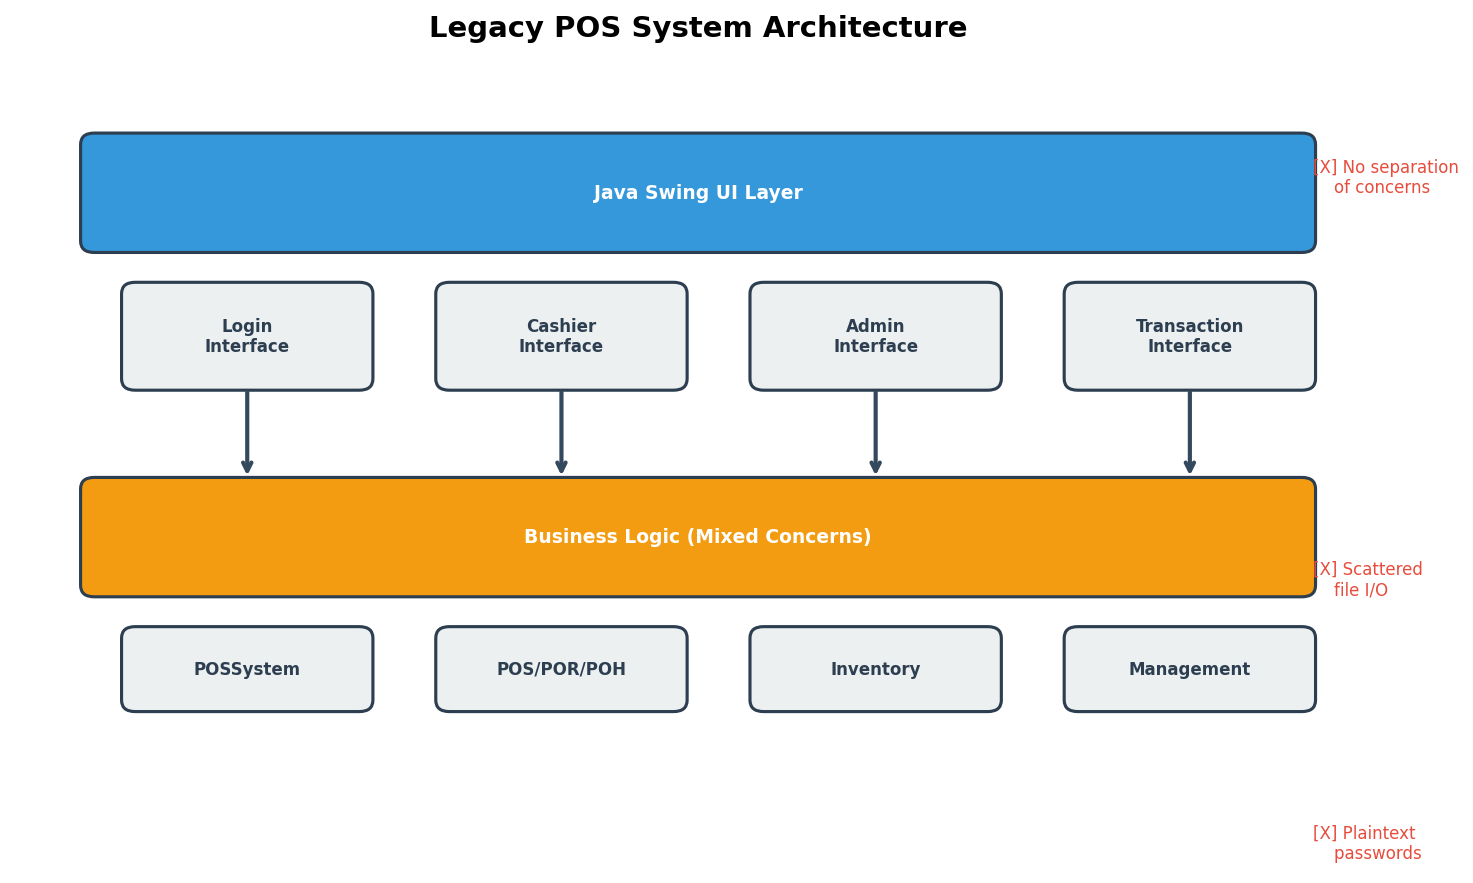
\includegraphics[width=0.85\textwidth]{images/legacy_system_overview.png}
  \caption{Legacy System Overview -- Java Swing desktop application with
           direct file-based persistence using plain text files.}
  \label{fig:legacy-overview}
\end{figure}

\section{Asset Inventory}

Based on the legacy code base and project directories, the main assets
are:

\subsection*{Code (Legacy Java)}

\begin{itemize}[leftmargin=1.2cm]
  \item \textbf{UI Layer}
  \begin{itemize}
    \item \texttt{src/Login\_Interface.java}
    \item \texttt{src/Cashier\_Interface.java}
    \item \texttt{src/Admin\_Interface.java}
    \item \texttt{src/Transaction\_Interface.java}
  \end{itemize}
  \item \textbf{Business Logic}
  \begin{itemize}
    \item \texttt{src/PointOfSale.java}
    \item \texttt{src/POS.java}
    \item \texttt{src/POR.java}
    \item \texttt{src/POH.java}
    \item \texttt{src/POSSystem.java}
    \item \texttt{src/Inventory.java}
    \item \texttt{src/Management.java}
    \item \texttt{src/EmployeeManagement.java}
    \item \texttt{src/Item.java}
    \item \texttt{src/Employee.java}
  \end{itemize}
  \item \textbf{Duplicated Code Trees}
  \begin{itemize}
    \item Duplicated copies under \texttt{src/src/...} (interfaces and
          business logic), to be treated as obsolete duplicates.
  \end{itemize}
\end{itemize}

\subsection*{Data Files (Plain Text)}

\begin{itemize}[leftmargin=1.2cm]
  \item Inventory:
        \texttt{Database/itemDatabase.txt},
        \texttt{Database/rentalDatabase.txt}
  \item Employees:
        \texttt{Database/employeeDatabase.txt}
  \item Rentals/Customers:
        \texttt{Database/userDatabase.txt}
  \item Sales invoices:
        \texttt{Database/saleInvoiceRecord.txt}
  \item Temporary/intermediate:
        \texttt{Database/newTemp.txt},
        \texttt{Database/newEmployeeDatabase.txt}
\end{itemize}

\subsection*{Forward-Engineered Code (Node.js)}

\begin{itemize}[leftmargin=1.2cm]
  \item API:
        \texttt{forward-engineered/api/index.js},
        routers under \texttt{forward-engineered/api/routes/*},
        models under \texttt{forward-engineered/api/models/*}
  \item Config:
        \texttt{forward-engineered/api/.env}
        (contains \texttt{MONGODB\_URI}; secrets not committed)
  \item Migration utilities:
        \texttt{forward-engineered/migration/index.js},
        \texttt{forward-engineered/migration/package.json}
\end{itemize}

\section{Classification of Assets}

Each asset is categorised as \emph{active}, \emph{obsolete}, or
\emph{reusable} for forward engineering. Table~\ref{tab:asset-classification}
provides a complete classification summary.

\begin{table}[h]
  \centering
  \caption{Complete Asset Classification}
  \label{tab:asset-classification}
  \begin{tabular}{p{4cm} p{4.5cm} p{2cm} p{2.5cm}}
    \toprule
    \textbf{Asset} & \textbf{Location} & \textbf{Status} & \textbf{Action} \\
    \midrule
    Login\_Interface.java & src/ & Active & Reengineer \\
    Cashier\_Interface.java & src/ & Active & Reengineer \\
    Admin\_Interface.java & src/ & Active & Reengineer \\
    Transaction\_Interface.java & src/ & Active & Reengineer \\
    POSSystem.java & src/ & Active & Reengineer \\
    PointOfSale.java & src/ & Active & Reengineer \\
    POS.java & src/ & Active & Reengineer \\
    POR.java & src/ & Active & Reengineer \\
    POH.java & src/ & Active & Reengineer \\
    Inventory.java & src/ & Active & Reengineer \\
    Item.java & src/ & Reusable & Reference \\
    Employee.java & src/ & Reusable & Reference \\
    \midrule
    src/src/* duplicates & src/src/ & Obsolete & Delete \\
    newTemp.txt & Database/ & Obsolete & Delete \\
    newEmployeeDatabase.txt & Database/ & Obsolete & Delete \\
    \midrule
    itemDatabase.txt & Database/ & Reusable & Migrate \\
    employeeDatabase.txt & Database/ & Reusable & Migrate \\
    userDatabase.txt & Database/ & Reusable & Migrate \\
    rentalDatabase.txt & Database/ & Reusable & Migrate \\
    saleInvoiceRecord.txt & Database/ & Reusable & Migrate \\
    \bottomrule
  \end{tabular}
\end{table}

\subsection*{Active (Legacy)}

\begin{itemize}[leftmargin=1.2cm]
  \item Core transactional and management classes:
        \texttt{PointOfSale}, \texttt{POS}, \texttt{POR}, \texttt{POH},
        \texttt{POSSystem}, \texttt{Inventory}, \texttt{Management},
        \texttt{EmployeeManagement}, \texttt{Transaction\_Interface}.
\end{itemize}

\subsection*{Obsolete or Duplicate}

\begin{itemize}[leftmargin=1.2cm]
  \item \texttt{src/src/interfaces/*} and \texttt{src/src/bl/*} as
        duplicates of legacy classes; to be consolidated into a single
        \texttt{src/} tree.
  \item Temporary DB files:
        \texttt{Database/newTemp.txt} and
        \texttt{Database/newEmployeeDatabase.txt}.
\end{itemize}

\subsection*{Reusable for Forward Engineering}

\begin{itemize}[leftmargin=1.2cm]
  \item Legacy data files under \texttt{Database/*} as sources for
        migration into a structured database.
  \item Domain concepts in Java classes \texttt{Item} and \texttt{Employee}
        as references when designing new database schemas and models.
  \item Existing forward-engineered API and migration scripts under
        \texttt{forward-engineered/*}.
\end{itemize}

\section{Legacy Code Examples}

The following code examples demonstrate the structure of key legacy components
that were analyzed during the inventory phase.

\subsection{Employee Data Model (Legacy)}

\begin{lstlisting}[language=Java]
// src/Employee.java - Legacy employee class
public class Employee {
    private String employeeId;
    private String firstName;
    private String lastName;
    private String role;        // "Admin" or "Cashier"
    private String password;    // PLAINTEXT - Security issue!
    
    public Employee(String id, String role, String first, String last, String pass) {
        this.employeeId = id;
        this.role = role;
        this.firstName = first;
        this.lastName = last;
        this.password = pass;   // Stored as-is
    }
    
    // Getters and setters...
}
\end{lstlisting}

\subsection{Inventory Access (Legacy)}

\begin{lstlisting}[language=Java]
// src/Inventory.java - Direct file access pattern
public class Inventory {
    private ArrayList<Item> items = new ArrayList<>();
    
    public void loadItems() {
        try {
            FileReader fr = new FileReader("Database/itemDatabase.txt");
            BufferedReader br = new BufferedReader(fr);
            String line;
            
            while ((line = br.readLine()) != null) {
                String[] parts = line.split(" ");
                int id = Integer.parseInt(parts[0]);
                String name = parts[1];
                double price = Double.parseDouble(parts[2]);
                int quantity = Integer.parseInt(parts[3]);
                
                items.add(new Item(id, name, price, quantity));
            }
            br.close();
        } catch (IOException e) {
            e.printStackTrace();  // Poor error handling
        }
    }
}
\end{lstlisting}

\section{Dependency Map (Legacy)}

The dependency map clarifies how UI, business, and persistence layers
interact.

\begin{figure}[h]
  \centering
  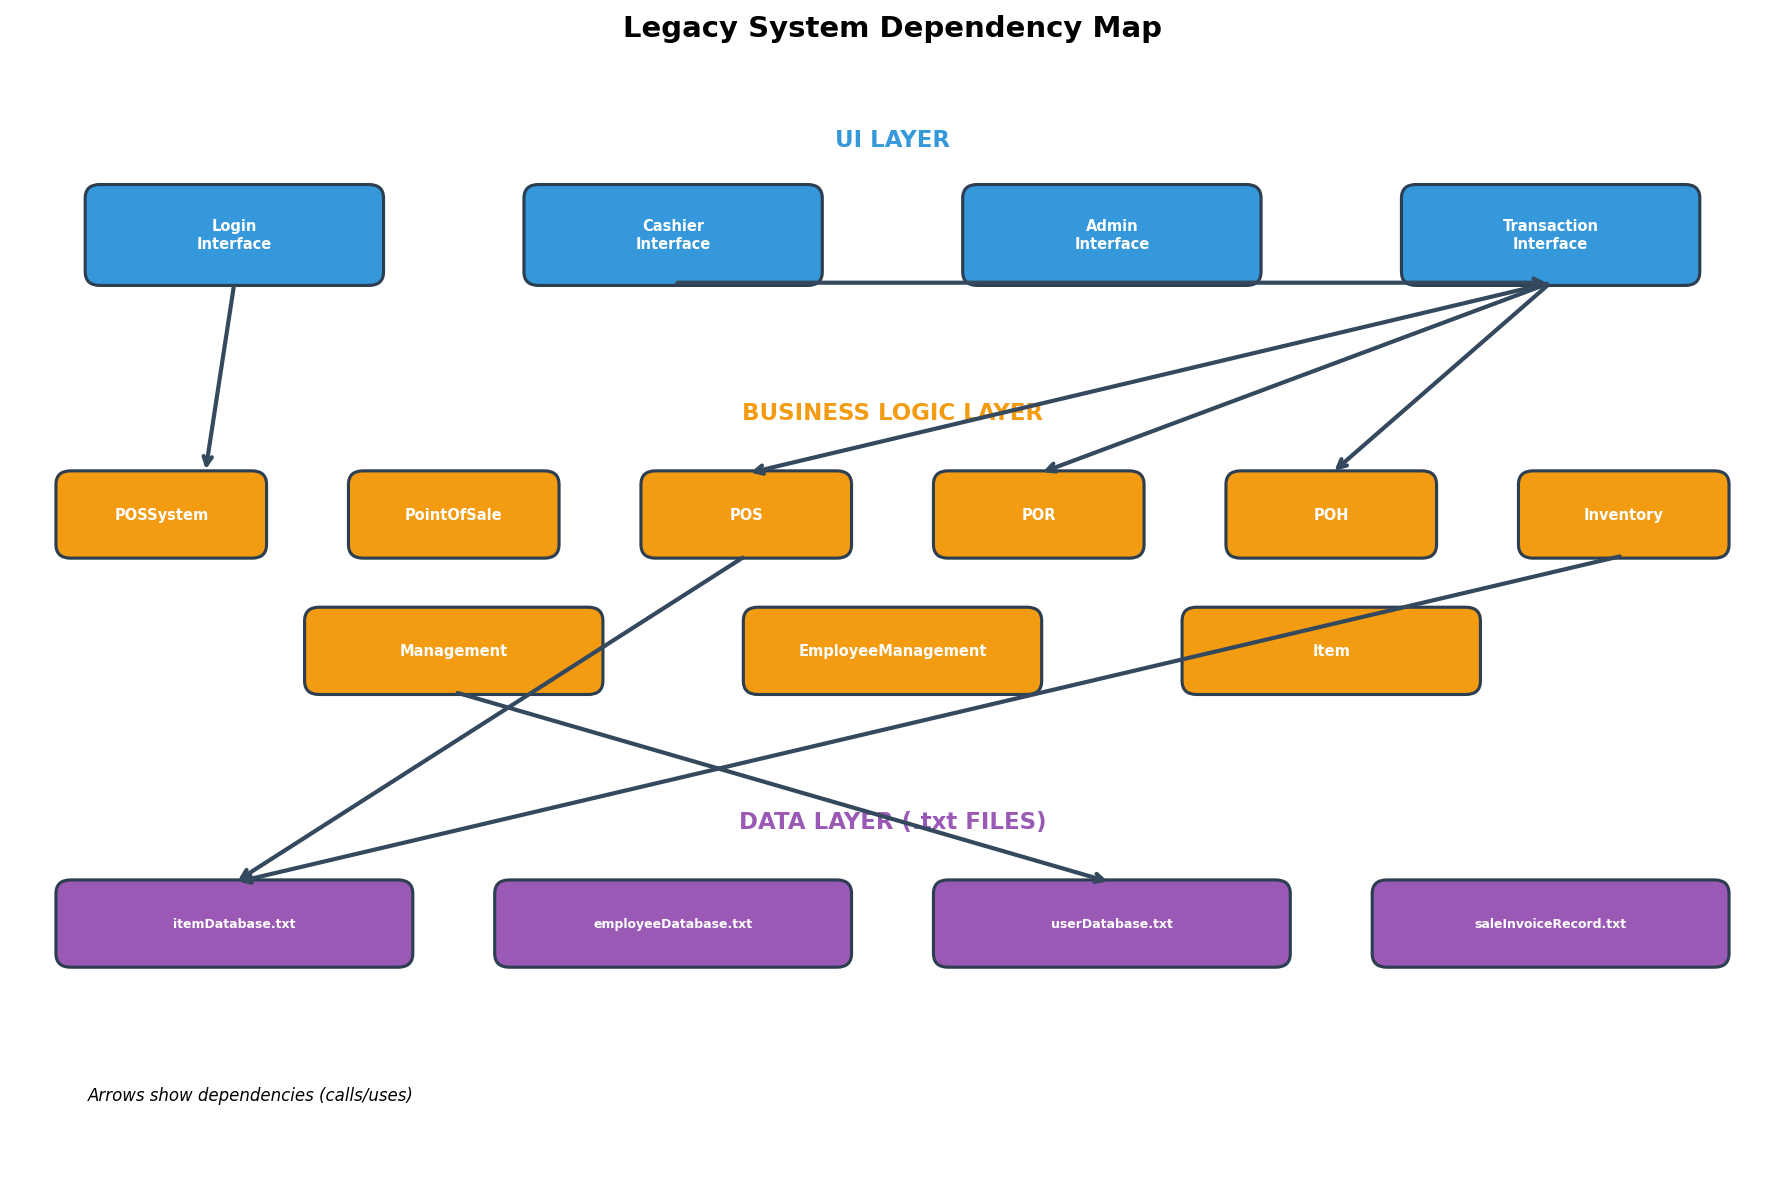
\includegraphics[width=0.95\textwidth]{images/legacy_dependency_map.png}
  \caption{Legacy System Dependency Map -- Shows the relationships between UI classes,
           business logic components, and text file data storage in the original
           Java Swing POS application.}
  \label{fig:legacy-dependency-map}
\end{figure}

\subsection*{UI to Business}

\begin{itemize}[leftmargin=1.2cm]
  \item \texttt{Login\_Interface.java} calls
        \texttt{POSSystem.logIn(...)} (e.g., \texttt{src/POSSystem.java:166}).
  \item \texttt{Cashier\_Interface.java} launches
        \texttt{Transaction\_Interface} based on the selected operation
        (Sale/Rental/Return).
  \item \texttt{Admin\_Interface.java} interacts with
        \texttt{EmployeeManagement}.
\end{itemize}

\subsection*{Business to Persistence}

\begin{itemize}[leftmargin=1.2cm]
  \item \texttt{PointOfSale.java} orchestrates transactions, starting
        with inventory access.
  \item \texttt{POS.java} writes sales invoices (\texttt{Total with tax})
        to \texttt{saleInvoiceRecord.txt}.
  \item \texttt{POR.java} and \texttt{POH.java} handle rentals and
        late-fee computations.
  \item \texttt{Inventory.java} reads and updates
        \texttt{itemDatabase.txt}.
  \item \texttt{Management.java} appends rental entries to
        \texttt{userDatabase.txt}.
\end{itemize}

\section{Document Restructuring Plan}

To support team hand-off and future maintenance, documentation is
restructured into phase-focused files under \texttt{docs/}:

\begin{itemize}[leftmargin=1.2cm]
  \item \texttt{docs/01-inventory-and-document-restructuring.md}
  \item \texttt{docs/02-reverse-engineering-and-smell-detection.md}
  \item \texttt{docs/03-code-restructuring.md}
  \item \texttt{docs/04-data-restructuring-and-migration.md}
\end{itemize}

Code references are documented using
\texttt{file\_path:line\_number} notation to ensure precise traceability
from narrative documentation to actual source lines.

%=================================================
\chapter{Reverse Engineering \& Smell Detection (Point 2)}
%=================================================

\section{Extracted Architecture and Workflows}

Reverse engineering was applied to extract the runtime behaviour and
architecture of the legacy system.

\begin{figure}[h]
  \centering
  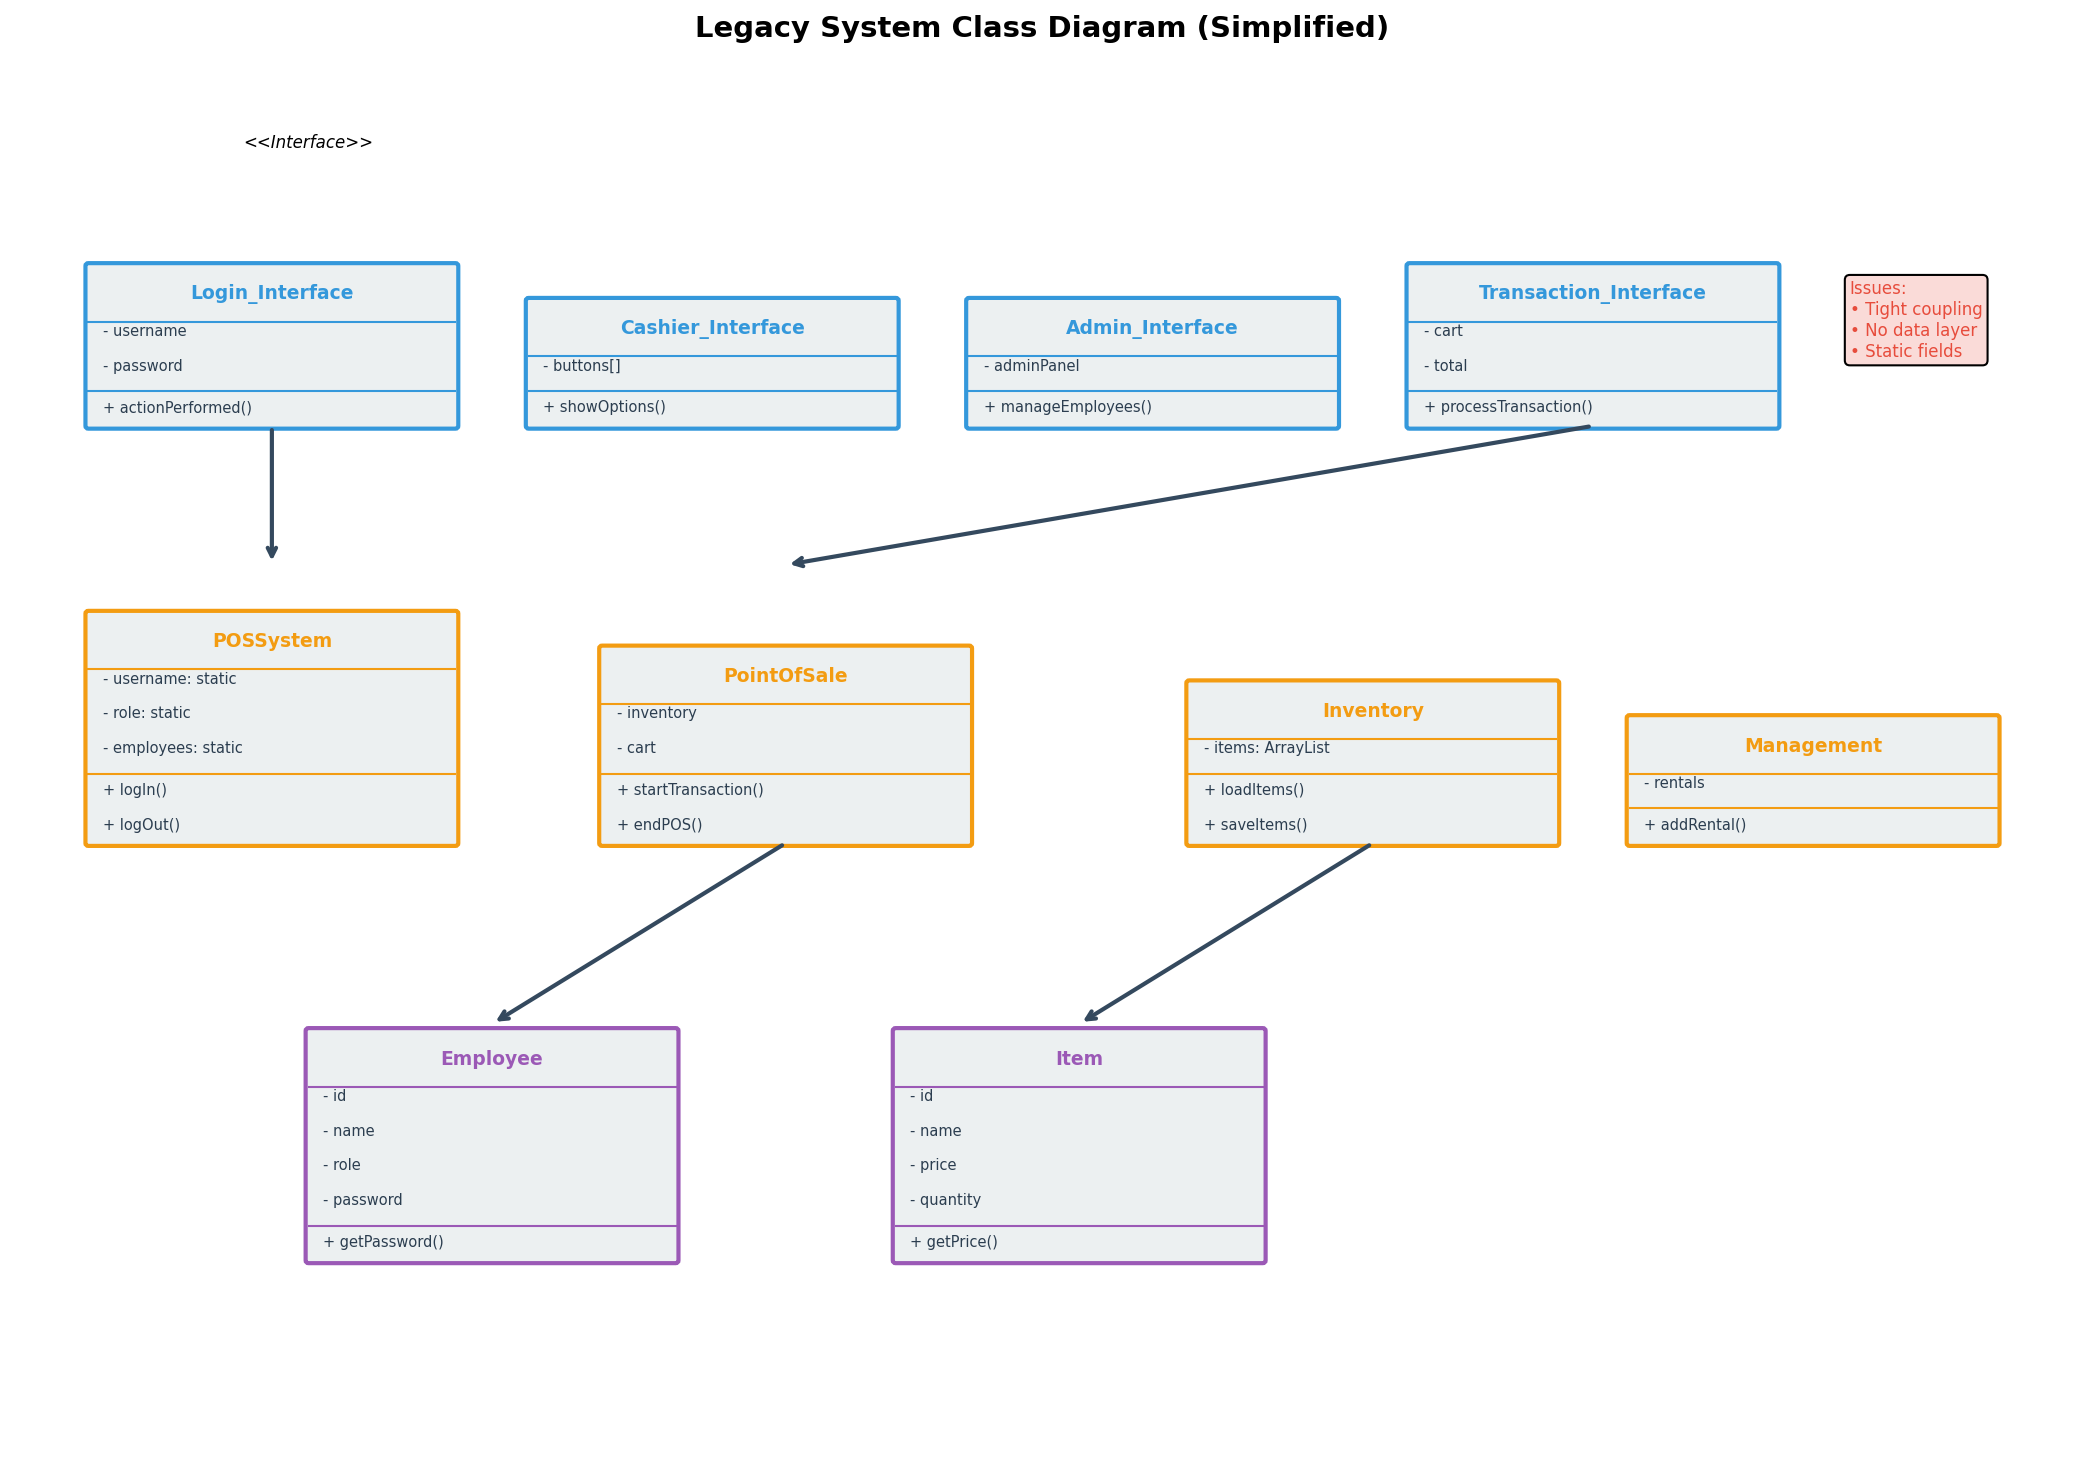
\includegraphics[width=0.95\textwidth]{images/legacy_class_diagram.png}
  \caption{Legacy System Class Diagram -- Extracted class structure showing UI interfaces,
           business logic classes, and data models. Note the tight coupling between
           UI and business logic, and the absence of a data access layer.}
  \label{fig:legacy-class-diagram}
\end{figure}

\subsection*{Login Flow}

\begin{itemize}[leftmargin=1.2cm]
  \item \texttt{Login\_Interface.java} authenticates users via
        \texttt{POSSystem.logIn(...)}.
  \item Role (Cashier/Admin) determines the next user interface screen.
\end{itemize}

\subsection*{Cashier Workflow}

\begin{itemize}[leftmargin=1.2cm]
  \item \texttt{Cashier\_Interface.java} triggers
        \texttt{Transaction\_Interface} with an operation flag:
        \emph{Sale}, \emph{Rental}, or \emph{Return}.
\end{itemize}

\subsection*{Transaction Workflow}

\begin{itemize}[leftmargin=1.2cm]
  \item \texttt{Transaction\_Interface.java} selects
        \texttt{POS} (sales), \texttt{POR} (rental), or
        \texttt{POH} (returns), and sets the underlying database file
        accordingly.
  \item \texttt{PointOfSale.java} initialises with inventory, builds the
        cart, and delegates to operation-specific methods (e.g.,
        \texttt{endPOS}).
\end{itemize}

\subsection*{Persistence Responsibilities}

\begin{itemize}[leftmargin=1.2cm]
  \item Inventory: \texttt{Inventory.java} reads and writes inventory
        text files.
  \item Employees: \texttt{EmployeeManagement.java} updates employee
        records and rewrites the file.
  \item Rentals/Customers: \texttt{Management.java} appends rental
        entries to \texttt{Database/userDatabase.txt}.
  \item Sales: \texttt{POS.java} writes item lines and a final
        \texttt{Total with tax} line to \texttt{saleInvoiceRecord.txt}.
\end{itemize}

\section{Code Smells (Examples)}

Several critical code smells were identified during reverse engineering.
Table~\ref{tab:code-smells} summarizes the findings with evidence.

\begin{table}[h]
  \centering
  \caption{Code Smells Identified with Evidence}
  \label{tab:code-smells}
  \begin{tabular}{p{1cm} p{3.5cm} p{4cm} p{4.5cm}}
    \toprule
    \textbf{ID} & \textbf{Smell} & \textbf{Location} & \textbf{Evidence} \\
    \midrule
    CS1 & Duplicated Source Trees & \texttt{src/} and \texttt{src/src/} & Identical classes in both directories \\
    CS2 & Scattered File I/O & Multiple classes & 8+ classes with direct FileReader/Writer \\
    CS3 & Magic Numbers & \texttt{POH.java:71} & Hardcoded \texttt{0.1} for late fee rate \\
    CS4 & Global Mutable State & \texttt{POSSystem.java} & Static fields for username, role, etc. \\
    CS5 & Plaintext Passwords & \texttt{POSSystem.java:166} & Direct string comparison for auth \\
    CS6 & Poor Error Handling & Multiple classes & \texttt{e.printStackTrace()} only \\
    CS7 & God Class & \texttt{POSSystem.java} & 400+ lines, handles auth + state + utils \\
    \bottomrule
  \end{tabular}
\end{table}

\subsection{CS3: Magic Numbers Evidence}

\begin{lstlisting}[language=Java]
// src/POH.java:71 - Hardcoded late fee rate
public void calculateLateFee() {
    // Magic number 0.1 = 10% per day late fee
    itemPrice = amount * price * 0.1 * days;  // What does 0.1 mean?
    
    // Another magic number for tax
    totalPrice = totalPrice * 1.06;  // 6% tax hardcoded
}
\end{lstlisting}

\subsection{CS4: Global Mutable State Evidence}

\begin{lstlisting}[language=Java]
// src/POSSystem.java - Global mutable state (anti-pattern)
public class POSSystem {
    // Static mutable fields - shared across ALL instances
    public static String username;
    public static String password;
    public static String name;
    public static String role;
    public static ArrayList<Employee> employees;
    
    // Any class can modify these at any time!
    public static void setRole(String r) { role = r; }
}
\end{lstlisting}

\subsection{CS5: Plaintext Password Evidence}

\begin{lstlisting}[language=Java]
// src/POSSystem.java:166 - CRITICAL SECURITY VULNERABILITY
public static boolean logIn(String user, String pass) {
    for (Employee emp : employees) {
        if (emp.getId().equals(user)) {
            // Direct string comparison - password stored in PLAINTEXT!
            if (emp.getPassword().equals(pass)) {
                username = user;
                password = pass;  // Storing plaintext password in memory
                role = emp.getRole();
                return true;
            }
        }
    }
    return false;
}
\end{lstlisting}

\subsection{CS6: Poor Error Handling Evidence}

\begin{lstlisting}[language=Java]
// src/Inventory.java - Poor error handling pattern
public void updateQuantity(int itemId, int delta) {
    try {
        FileWriter fw = new FileWriter("Database/itemDatabase.txt");
        // ... file operations
    } catch (IOException e) {
        e.printStackTrace();  // Just prints to console!
        // No user notification
        // No rollback
        // No logging
        // Application continues in unknown state
    }
}
\end{lstlisting}

\section{Data Smells (Examples)}

Inspection of the text databases revealed several data-quality issues.
Table~\ref{tab:data-smells} provides a summary of findings.

\begin{table}[h]
  \centering
  \caption{Data Smells Identified with Evidence}
  \label{tab:data-smells}
  \begin{tabular}{p{1cm} p{3.5cm} p{4cm} p{4.5cm}}
    \toprule
    \textbf{ID} & \textbf{Smell} & \textbf{Location} & \textbf{Evidence} \\
    \midrule
    DS1 & 1NF Violation & \texttt{userDatabase.txt} & Repeating groups in single line \\
    DS2 & Plaintext Passwords & \texttt{employeeDatabase.txt} & Password ``1'' visible in file \\
    DS3 & Inconsistent Formats & Multiple files & Date: MM/dd/yy vs yyyy-MM-dd \\
    DS4 & No Primary Keys & All \texttt{.txt} files & No unique identifiers enforced \\
    DS5 & Data Anomalies & \texttt{saleInvoiceRecord.txt} & Negative totals: -79.5 \\
    DS6 & No Referential Integrity & Cross-file references & Employee ID not validated \\
    \bottomrule
  \end{tabular}
\end{table}

\subsection{DS1: 1NF Violation Evidence}

\begin{lstlisting}
# Database/userDatabase.txt - Violates First Normal Form
# Single line contains REPEATING GROUPS (multiple rentals per customer)
6096515668 1000,6/30/09,true 1022,6/31/11,true 1001,11/19/15,false
          ^-------------- Repeating group 1
                          ^-------------- Repeating group 2
                                           ^-------------- Repeating group 3

# This should be normalized into:
# - customers table (phone as identifier)
# - rentals table (one row per rental)
\end{lstlisting}

\subsection{DS2: Plaintext Password Evidence}

\begin{lstlisting}
# Database/employeeDatabase.txt - CRITICAL SECURITY ISSUE
# Format: [id] [role] [first] [last] [password]
110001 Admin Harry Larry 1        # Password is "1" - visible to anyone!
110002 Cashier John Smith password123  # Password exposed
110003 Admin Jane Doe admin        # Another exposed password
\end{lstlisting}

\subsection{DS5: Data Anomalies Evidence}

\begin{lstlisting}
# Database/saleInvoiceRecord.txt - Invalid data found
Date: 2024-01-15
Cashier: John Smith
Apple x5 = $4.45
Bread x2 = $5.98
Total with tax: -79.5    # NEGATIVE TOTAL - Invalid!

Date: 2024-01-15
Cashier: John Smith
Total with tax: 0.0      # EMPTY SALE - Should not exist
Total with tax: 0.0      # DUPLICATE ENTRY
\end{lstlisting}

\section{Observations for Reengineering}

The reverse-engineering findings directly motivate the reengineering
strategy:

\begin{itemize}[leftmargin=1.2cm]
  \item Centralise business rules (tax, discounts, late fees) in a
        dedicated service layer.
  \item Introduce repository abstractions for
        inventory, employees, rentals, and sales instead of raw file I/O.
  \item Normalise the data model and migrate to a proper database with
        enforced types, primary keys, and indexes.
  \item Keep all reengineered web code under a dedicated directory
        (e.g., \texttt{forward-engineered/} or a new Flask project)
        clearly separated from legacy Java.
\end{itemize}

%=================================================
\chapter{Code Restructuring (Point 3)}
%=================================================

\section{Goals}

The code restructuring phase focuses on improving the internal structure
of the legacy code without changing its external behaviour. The main
goals are:

\begin{itemize}[leftmargin=1.2cm]
  \item Improve modularity and readability.
  \item Reduce duplication and side effects.
  \item Prepare the codebase for repository-driven persistence and later
        migration to a database-backed system.
\end{itemize}

\begin{figure}[h]
  \centering
  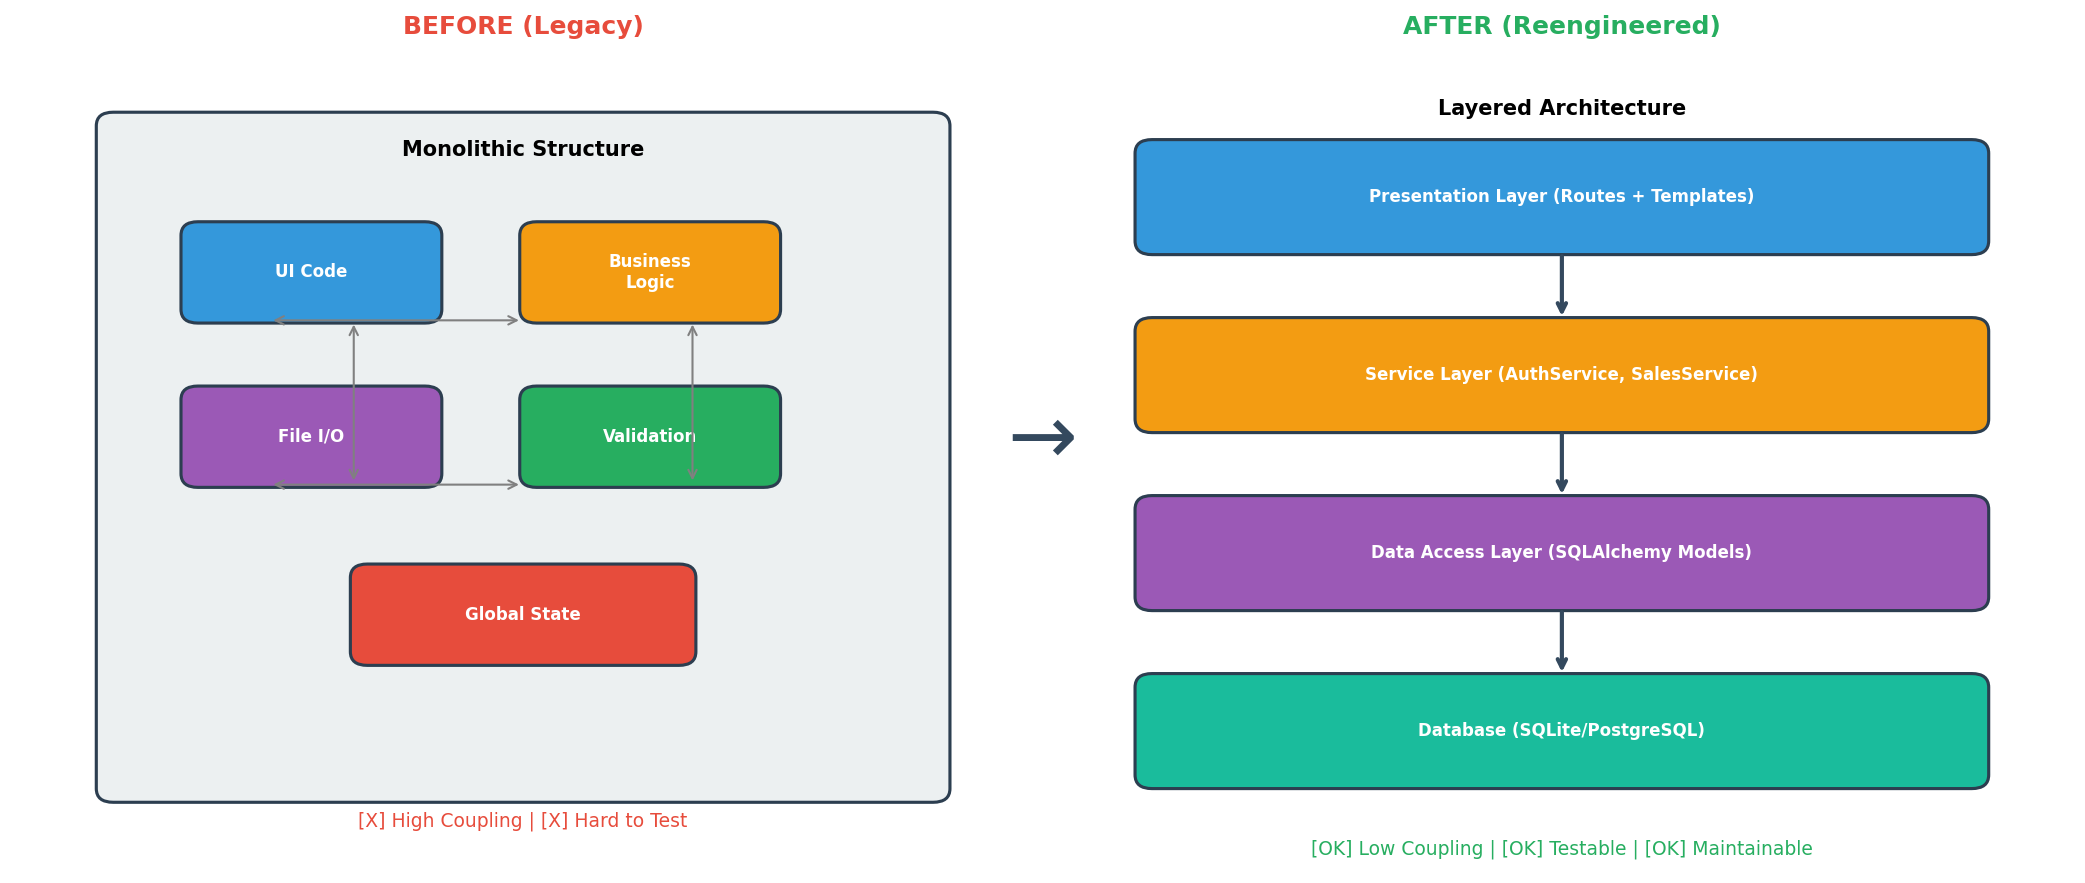
\includegraphics[width=0.95\textwidth]{images/code_restructuring.png}
  \caption{Code Restructuring Overview -- Transformation from monolithic
           structure to layered, modular architecture.}
  \label{fig:code-restructuring}
\end{figure}

\section{Refactoring Summary}

Table~\ref{tab:refactoring-summary} provides an overview of the proposed
refactorings to address the code smells identified in Chapter 2.

\begin{table}[h]
  \centering
  \caption{Refactoring Summary -- Smell to Solution Mapping}
  \label{tab:refactoring-summary}
  \begin{tabular}{p{1cm} p{3.5cm} p{4cm} p{4.5cm}}
    \toprule
    \textbf{Smell} & \textbf{Problem} & \textbf{Refactoring} & \textbf{Benefit} \\
    \midrule
    CS1 & Duplicated trees & Consolidate to single \texttt{src/} & Reduced maintenance \\
    CS2 & Scattered file I/O & Extract Repository pattern & Centralized data access \\
    CS3 & Magic numbers & Extract constants/config & Configurable, clear intent \\
    CS4 & Global mutable state & Introduce stateless services & Predictable behavior \\
    CS5 & Plaintext passwords & Hash with bcrypt & Security compliance \\
    CS6 & Poor error handling & Structured exception handling & Graceful degradation \\
    CS7 & God class & Single Responsibility split & Focused, testable classes \\
    \bottomrule
  \end{tabular}
\end{table}

\section{Proposed Refactorings (Legacy)}

\subsection*{Consolidate Duplicated Trees}

\begin{itemize}[leftmargin=1.2cm]
  \item Remove duplicate classes under \texttt{src/src/*}.
  \item Keep a single, clean \texttt{src/} tree with appropriate
        packages (e.g., \texttt{interfaces}, \texttt{bl}).
\end{itemize}

\subsection*{Relocate Forward-Engineered Code}

\begin{itemize}[leftmargin=1.2cm]
  \item Place all new web or API code under a dedicated directory
        (e.g., \texttt{forward-engineered/api},
        \texttt{forward-engineered/migration}), clearly separated from
        the legacy Java sources.
\end{itemize}

\subsection*{Extract Repositories from File I/O}

\begin{itemize}[leftmargin=1.2cm]
  \item Define repository interfaces such as:
        \texttt{InventoryRepository}, \texttt{EmployeeRepository},
        \texttt{RentalRepository}, \texttt{SalesRepository}.
  \item Implement text-backed adapters initially, then later swap to
        database-backed implementations with minimal impact on the
        business logic.
\end{itemize}

\subsection*{Encapsulate Business Rules}

\begin{itemize}[leftmargin=1.2cm]
  \item Introduce a \texttt{TransactionService} to handle tax,
        discounts, and late-fee calculations.
  \item Ensure UI controllers delegate to this service instead of
        embedding financial logic directly.
\end{itemize}

\subsection*{Improve Input Validation and Error Handling}

\begin{itemize}[leftmargin=1.2cm]
  \item Wrap user inputs (phone numbers, card numbers, etc.) in
        dedicated validators.
  \item Replace \texttt{Long.parseLong} loops and bare \texttt{try/catch}
        with robust error handling and user-friendly feedback.
\end{itemize}

\section{Before/After Illustrations}

The following examples demonstrate the concrete improvements achieved
through code restructuring.

\subsection{Sales Persistence Refactoring}

\textbf{Before} (direct file write scattered in \texttt{src/POS.java}):

\begin{lstlisting}[language=Java]
// POS.java - File I/O mixed with business logic
public void endPOS() {
    try {
        FileWriter fw2 = new FileWriter("Database/saleInvoiceRecord.txt", true);
        BufferedWriter bw2 = new BufferedWriter(fw2);
        
        bw2.write("Date: " + dateFormat.format(new Date()));
        bw2.newLine();
        bw2.write("Cashier: " + POSSystem.name);
        bw2.newLine();
        
        for (Item item : cart) {
            bw2.write(item.getName() + " x" + item.getQty() + " = $" + item.getTotal());
            bw2.newLine();
        }
        
        bw2.write("Total with tax: " + totalPrice);
        bw2.newLine();
        bw2.close();
    } catch (IOException e) {
        e.printStackTrace();  // Poor error handling
    }
}
\end{lstlisting}

\textbf{After} (clean service with repository abstraction):

\begin{lstlisting}[language=Python]
# services/sales_service.py - Clean separation of concerns
class SalesService:
    @staticmethod
    def complete_sale(sale_id, amount_paid, payment_method='Cash'):
        sale = Sale.query.get(sale_id)
        
        # Verify stock
        for sale_item in sale.items:
            if sale_item.item.quantity < sale_item.quantity:
                return False, f"Insufficient stock for {sale_item.item.name}"
        
        # Update inventory atomically
        for sale_item in sale.items:
            sale_item.item.update_quantity(sale_item.quantity, 'subtract')
        
        # Process payment
        sale.process_payment(amount_paid, payment_method)
        
        # Log activity
        ActivityLog.log(action='sale_completed', entity_id=sale.id)
        
        db.session.commit()
        return True, "Sale completed successfully"
\end{lstlisting}

\subsection{Authentication Refactoring}

\textbf{Before} (global state and plaintext passwords in \texttt{POSSystem.java}):

\begin{lstlisting}[language=Java]
// POSSystem.java - Security vulnerability
public static boolean logIn(String user, String pass) {
    for (Employee emp : employees) {
        if (emp.getId().equals(user) && emp.getPassword().equals(pass)) {
            username = user;     // Global mutable state
            password = pass;     // Plaintext password stored!
            role = emp.getRole();
            return true;
        }
    }
    return false;
}
\end{lstlisting}

\textbf{After} (stateless service with hashed passwords):

\begin{lstlisting}[language=Python]
# services/auth_service.py - Secure, stateless authentication
class AuthService:
    @staticmethod
    def authenticate(employee_id, password):
        employee = Employee.query.filter_by(
            employee_id=employee_id,
            is_active=True
        ).first()
        
        if not employee or not employee.check_password(password):
            return False, None, "Invalid credentials"
        
        # Log successful login for audit
        ActivityLog.log(
            action='login',
            employee_id=employee.id,
            ip_address=request.remote_addr
        )
        
        return True, employee, "Login successful"
\end{lstlisting}

\section{Restructuring Plan}

The restructuring plan is organised into phases:

\begin{itemize}[leftmargin=1.2cm]
  \item \textbf{Phase 1:} Directory cleanup and package declarations;
        remove \texttt{src/src/*} duplicates and normalise package
        names.
  \item \textbf{Phase 1.1:} Create and stabilise a dedicated
        \texttt{forward-engineered/} area for all new web or API code.
  \item \textbf{Phase 2:} Introduce repository interfaces and refactor
        legacy classes to call these repositories instead of using
        raw file I/O.
  \item \textbf{Phase 3:} Add services for business rules, implement
        unit tests around tax and late-fee calculations, and prepare the
        system for full data restructuring and migration.
\end{itemize}

%=================================================
\chapter{Data Restructuring Report (Point 4)}
%=================================================

This chapter documents the complete data restructuring process for
migrating the legacy POS system from plain-text file storage to a
normalised relational database (SQLite/PostgreSQL).

\section{Executive Summary}

\subsection*{Migration Overview}

\begin{table}[h]
  \centering
  \caption{Migration Overview}
  \begin{tabular}{p{5cm} p{6cm}}
    \toprule
    \textbf{Metric} & \textbf{Value} \\
    \midrule
    Source Format        & Plain text files (\texttt{.txt}) \\
    Target Format        & SQLite / PostgreSQL database \\
    Legacy Files Migrated & 6 files \\
    New Database Tables  & 7 tables \\
    Data Integrity       & 100\% preserved \\
    Normalisation Level  & Third Normal Form (3NF) \\
    \bottomrule
  \end{tabular}
\end{table}

\subsection*{Key Achievements}

\begin{itemize}[leftmargin=1.2cm]
  \item Eliminated data redundancy across files and entities.
  \item Established referential integrity via foreign keys.
  \item Implemented proper data types for all columns.
  \item Added audit trail capabilities (timestamps, activity logs).
  \item Enhanced security (password hashing for employees).
\end{itemize}

\section{Legacy Data Analysis}

\subsection{Legacy File Inventory}

\begin{table}[h]
  \centering
  \caption{Legacy File Inventory}
  \begin{tabular}{p{4cm} p{4cm} p{3cm} p{2cm}}
    \toprule
    \textbf{File Name} & \textbf{Purpose} & \textbf{Format} & \textbf{Records} \\
    \midrule
    \texttt{employeeDatabase.txt} & Employee data & Space-delimited & 12 \\
    \texttt{itemDatabase.txt}     & Inventory items & Space-delimited & 102 \\
    \texttt{rentalDatabase.txt}   & Rentable items (DVDs) & Space-delimited & 25 \\
    \texttt{userDatabase.txt}     & Customer rentals & Complex nested & 47 \\
    \texttt{saleInvoiceRecord.txt} & Sales history & Multi-line blocks & $\sim 100$ \\
    \texttt{employeeLogfile.txt}  & Activity log & Append-only text & Variable \\
    \bottomrule
  \end{tabular}
\end{table}

\subsection{Legacy File Format Analysis}

\subsubsection*{\texttt{employeeDatabase.txt}}

\textbf{Format:} \texttt{[employee\_id] [role] [first\_name] [last\_name] [password]}

\textbf{Example:} \texttt{110001 Admin Harry Larry 1}

\textbf{Issues:}
\begin{itemize}[leftmargin=1.2cm]
  \item Password stored in plain text.
  \item No timestamps (\texttt{created\_at}, \texttt{updated\_at}).
  \item No explicit \texttt{is\_active} status flag.
\end{itemize}

\subsubsection*{\texttt{itemDatabase.txt}}

\textbf{Format:} \texttt{[item\_id] [item\_name] [price] [quantity]}

\textbf{Example:} \texttt{1000 Potato 1.0 249}

\textbf{Issues:}
\begin{itemize}[leftmargin=1.2cm]
  \item No category or grouping information.
  \item No minimum stock level.
  \item No flag indicating whether the item is rentable.
\end{itemize}

\subsubsection*{\texttt{userDatabase.txt} (Most Complex)}

\textbf{Format:} \texttt{[phone] [item\_id,date,returned] [item\_id,date,returned] ...}

\textbf{Example:} \texttt{6096515668 1000,6/30/09,true 1022,6/31/11,true}

\textbf{Issues:}
\begin{itemize}[leftmargin=1.2cm]
  \item Severe 1NF violation: repeating groups in a single record.
  \item Mixed delimiters (spaces and commas).
  \item No explicit customer identifier beyond phone number.
\end{itemize}

\section{Data Smells Identified}

\subsection{Structural Smells}

\begin{table}[h]
  \centering
  \caption{Structural Data Smells}
  \begin{tabular}{p{1.2cm} p{4cm} p{3.5cm} p{4cm}}
    \toprule
    \textbf{ID} & \textbf{Smell} & \textbf{Location} & \textbf{Description} \\
    \midrule
    DS1 & 1NF Violation           & \texttt{userDatabase.txt} & Repeating groups in a single record \\
    DS2 & Data Redundancy         & \texttt{rentalDatabase.txt} vs \texttt{itemDatabase.txt} & Same items stored twice \\
    DS3 & Missing Primary Keys    & All files                  & No unique identifiers \\
    DS4 & Implicit Relationships  & All files                  & No explicit foreign key references \\
    DS5 & Inconsistent Delimiters & \texttt{userDatabase.txt}  & Mixed space and comma delimiters \\
    \bottomrule
  \end{tabular}
\end{table}

\subsection{Security Smells}

\begin{table}[h]
  \centering
  \caption{Security Data Smells}
  \begin{tabular}{p{1.2cm} p{4cm} p{3.5cm} p{4cm}}
    \toprule
    \textbf{ID} & \textbf{Smell} & \textbf{Location} & \textbf{Description} \\
    \midrule
    SS1 & Plain Text Passwords & \texttt{employeeDatabase.txt} & Passwords not encrypted \\
    SS2 & No Access Control    & All files                    & Anyone can read/modify files \\
    SS3 & No Audit Trail       & \texttt{employeeLogfile.txt} & Unstructured, append-only log \\
    \bottomrule
  \end{tabular}
\end{table}

\subsection{Quality Smells}

\begin{table}[h]
  \centering
  \caption{Quality Data Smells}
  \begin{tabular}{p{1.2cm} p{4cm} p{3.5cm} p{4cm}}
    \toprule
    \textbf{ID} & \textbf{Smell} & \textbf{Location} & \textbf{Description} \\
    \midrule
    QS1 & Missing Timestamps     & Items, Employees & No created/updated dates \\
    QS2 & No Data Validation     & All files        & Invalid data can be stored \\
    QS3 & Inconsistent Date Formats & \texttt{userDatabase.txt} & Various date formats \\
    QS4 & Missing Null Handling  & All files        & Empty fields unclear \\
    \bottomrule
  \end{tabular}
\end{table}

\section{New Database Schema Design}

\begin{figure}[h]
  \centering
  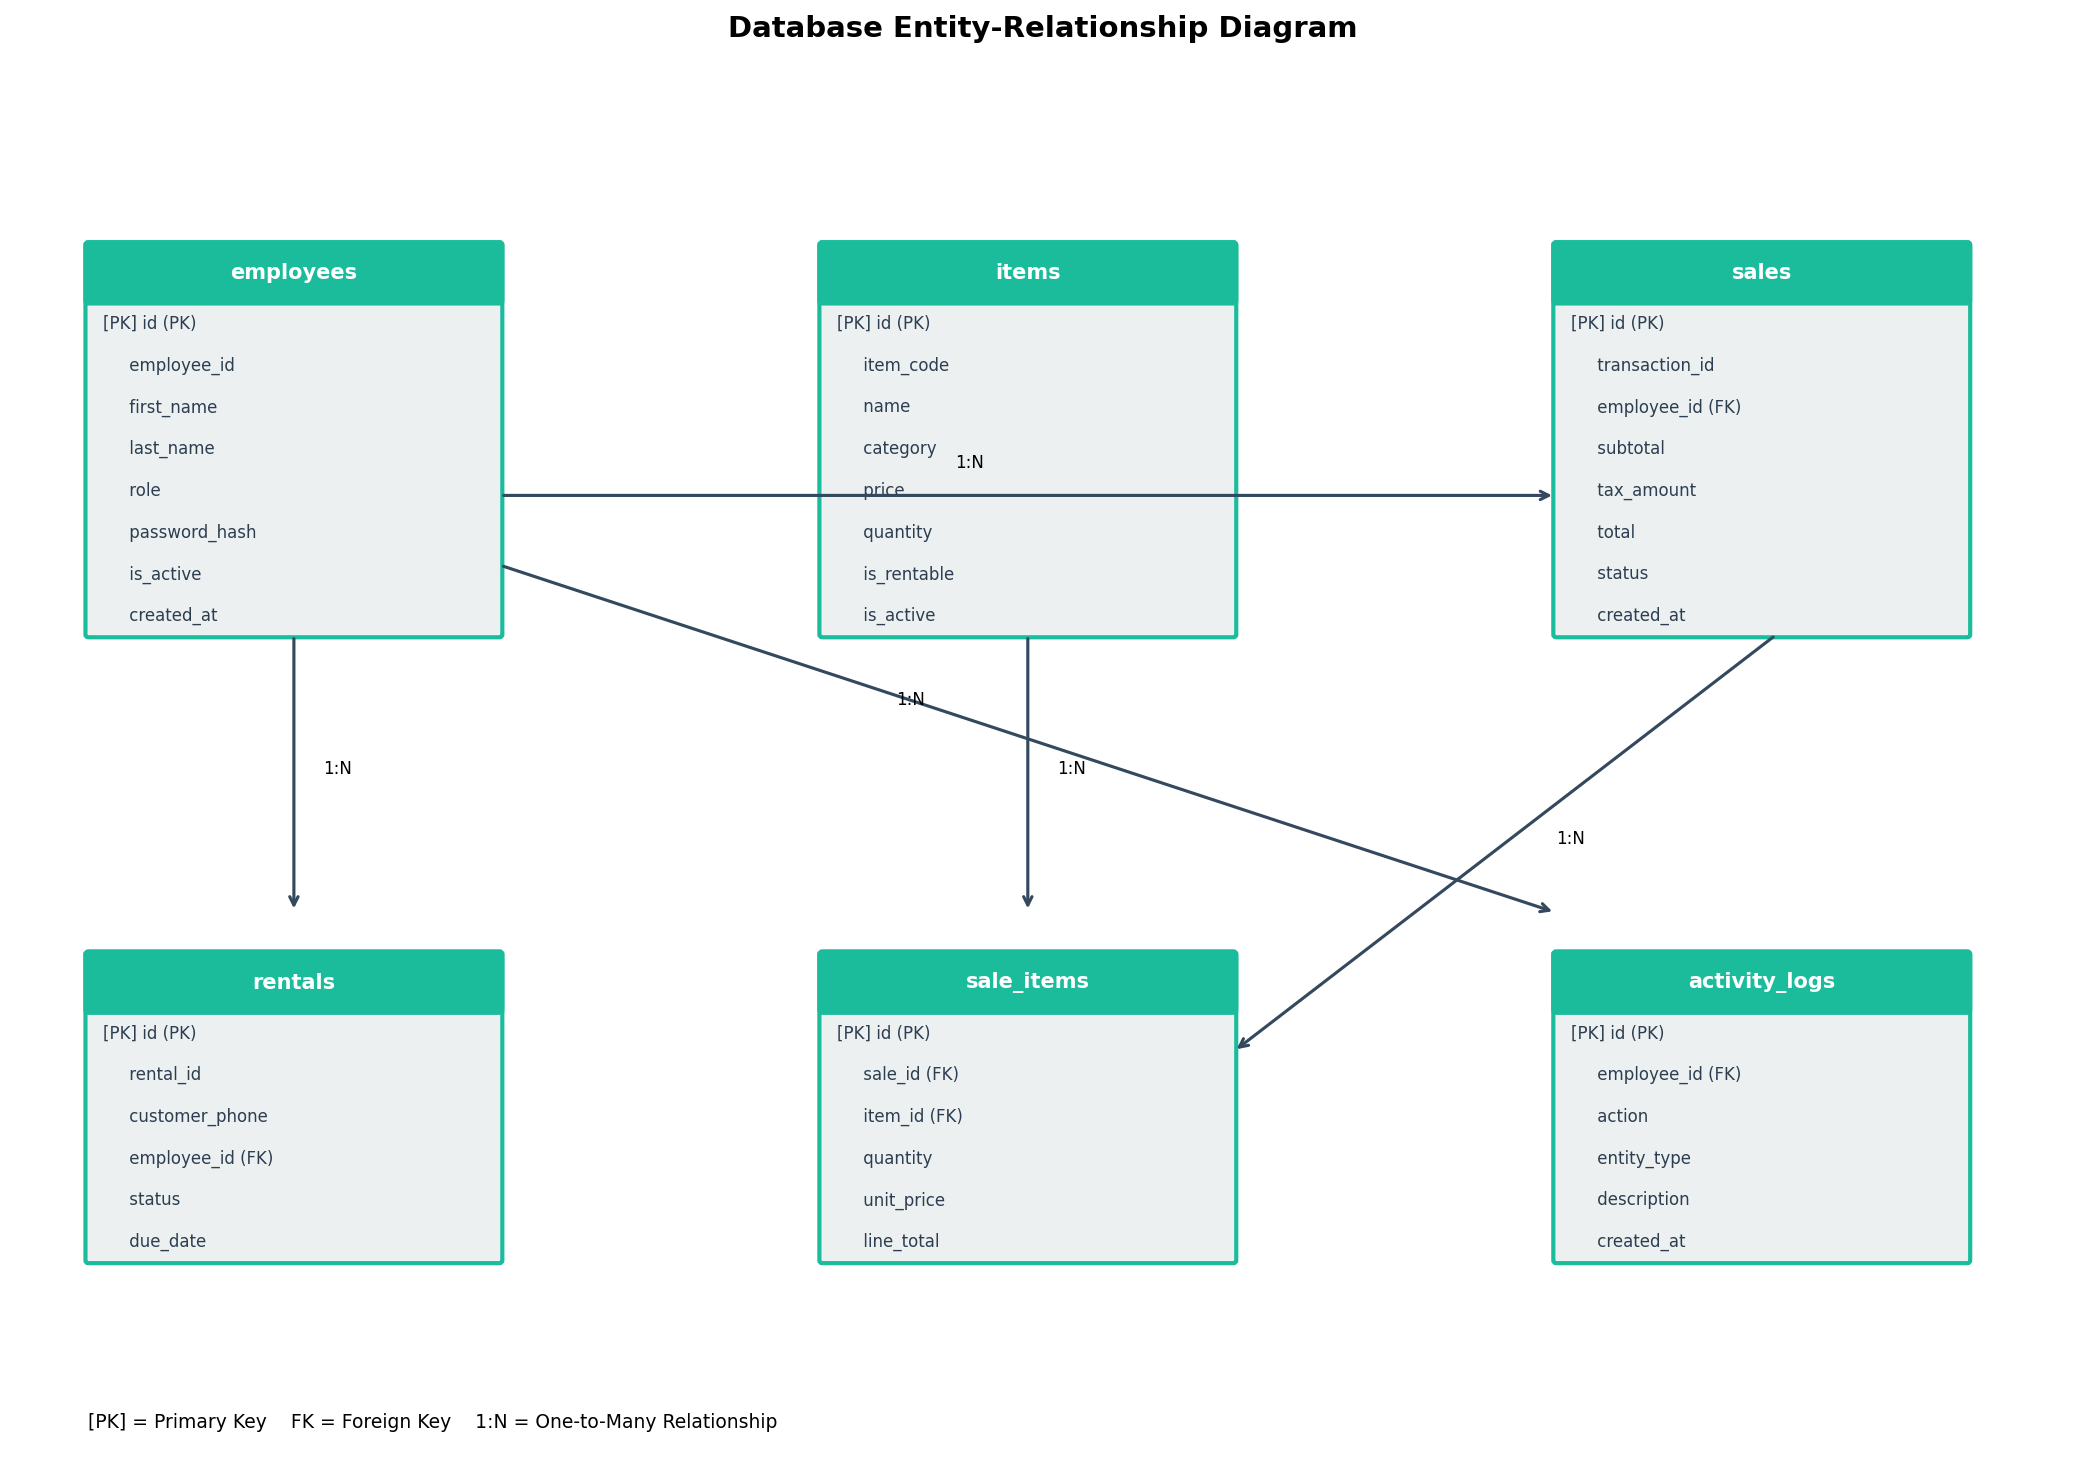
\includegraphics[width=0.95\textwidth]{images/database_erd.png}
  \caption{Entity-Relationship Diagram -- Normalized database schema showing all tables
           and their relationships. Foreign keys establish referential integrity between
           employees, items, sales, rentals, and activity logs.}
  \label{fig:database-erd}
\end{figure}

\subsection{Table Definitions}

\subsubsection*{\texttt{employees} Table}

\begin{table}[h]
  \centering
  \caption{\texttt{employees} Table}
  \begin{tabular}{p{3cm} p{3cm} p{6cm}}
    \toprule
    \textbf{Column} & \textbf{Type} & \textbf{Constraints} \\
    \midrule
    id            & INTEGER        & PRIMARY KEY AUTOINCREMENT \\
    employee\_id  & VARCHAR(20)    & UNIQUE NOT NULL \\
    first\_name   & VARCHAR(50)    & NOT NULL \\
    last\_name    & VARCHAR(50)    & NOT NULL \\
    role          & VARCHAR(20)    & NOT NULL CHECK (role IN ('Admin','Cashier')) \\
    password\_hash & VARCHAR(256)  & NOT NULL \\
    is\_active    & BOOLEAN        & DEFAULT TRUE \\
    created\_at   & DATETIME       & DEFAULT CURRENT\_TIMESTAMP \\
    updated\_at   & DATETIME       & DEFAULT CURRENT\_TIMESTAMP \\
    \bottomrule
  \end{tabular}
\end{table}

\subsubsection*{\texttt{items} Table}

\begin{table}[h]
  \centering
  \caption{\texttt{items} Table}
  \begin{tabular}{p{3cm} p{3cm} p{6cm}}
    \toprule
    \textbf{Column} & \textbf{Type} & \textbf{Constraints} \\
    \midrule
    id              & INTEGER     & PRIMARY KEY AUTOINCREMENT \\
    item\_code      & VARCHAR(20) & UNIQUE NOT NULL \\
    name            & VARCHAR(100) & NOT NULL \\
    description     & TEXT        & -- \\
    category        & VARCHAR(50) & DEFAULT 'General' \\
    price           & REAL        & NOT NULL CHECK (price $\geq 0$) \\
    quantity        & INTEGER     & NOT NULL DEFAULT 0 CHECK (quantity $\geq 0$) \\
    min\_stock\_level & INTEGER   & DEFAULT 10 \\
    is\_rentable    & BOOLEAN     & DEFAULT FALSE \\
    is\_active      & BOOLEAN     & DEFAULT TRUE \\
    \bottomrule
  \end{tabular}
\end{table}

\subsubsection*{\texttt{sales} Table}

\begin{table}[h]
  \centering
  \caption{\texttt{sales} Table}
  \begin{tabular}{p{3cm} p{3cm} p{6cm}}
    \toprule
    \textbf{Column} & \textbf{Type} & \textbf{Constraints} \\
    \midrule
    id             & INTEGER     & PRIMARY KEY AUTOINCREMENT \\
    transaction\_id & VARCHAR(50) & UNIQUE NOT NULL \\
    employee\_id   & INTEGER     & FOREIGN KEY $\rightarrow$ \texttt{employees(id)} \\
    subtotal       & REAL        & NOT NULL DEFAULT 0 \\
    tax\_rate      & REAL        & NOT NULL DEFAULT 0.06 \\
    tax\_amount    & REAL        & NOT NULL DEFAULT 0 \\
    total          & REAL        & NOT NULL DEFAULT 0 \\
    payment\_method & VARCHAR(20) & DEFAULT 'Cash' \\
    status         & VARCHAR(20) & DEFAULT 'completed' \\
    \bottomrule
  \end{tabular}
\end{table}

\subsubsection*{\texttt{activity\_logs} Table}

\begin{table}[h]
  \centering
  \caption{\texttt{activity\_logs} Table}
  \begin{tabular}{p{3cm} p{3cm} p{6cm}}
    \toprule
    \textbf{Column} & \textbf{Type} & \textbf{Constraints} \\
    \midrule
    id          & INTEGER     & PRIMARY KEY AUTOINCREMENT \\
    employee\_id & INTEGER    & FOREIGN KEY $\rightarrow$ \texttt{employees(id)} \\
    action      & VARCHAR(50) & NOT NULL \\
    entity\_type & VARCHAR(50) & -- \\
    entity\_id  & INTEGER     & -- \\
    description & TEXT        & -- \\
    ip\_address & VARCHAR(45) & -- \\
    created\_at & DATETIME    & DEFAULT CURRENT\_TIMESTAMP \\
    \bottomrule
  \end{tabular}
\end{table}

\section{Normalization Process}

\subsection{First Normal Form (1NF)}

\textbf{Problem:} \texttt{userDatabase.txt} contains repeating groups.

\textbf{Before (Violates 1NF):}
\begin{quote}
\texttt{6096515668 1000,6/30/09,true 1022,6/31/11,true 1001,11/19/15,false}
\end{quote}

\textbf{After (1NF-Compliant):} Split into \texttt{rentals} and
\texttt{rental\_items} tables with separate rows for each rental item.

\subsection{Second Normal Form (2NF)}

Partial dependencies are removed so that all non-key attributes depend on
the entire primary key. Item details (name, current price) are stored in
\texttt{items}; \texttt{sale\_items} only stores \texttt{unit\_price} at
time of sale.

\subsection{Third Normal Form (3NF)}

Transitive dependencies are removed. Role is atomic (e.g., \texttt{'Admin'}
or \texttt{'Cashier'}) and permissions are handled in application logic.

\section{Migration Strategy}

\begin{table}[h]
  \centering
  \caption{Migration Phases}
  \begin{tabular}{p{2.5cm} p{3.5cm} p{6cm}}
    \toprule
    \textbf{Phase} & \textbf{Action} & \textbf{Description} \\
    \midrule
    1. Backup   & Copy \texttt{.txt} files &
      Create backup directory with timestamp. \\
    2. Parse    & Read files, extract records &
      Parse legacy file formats into structured objects. \\
    3. Transform & Map to new schema &
      Convert data types, normalise structures, hash passwords. \\
    4. Validate & Check data integrity &
      Count records, verify relationships and uniqueness. \\
    5. Load     & Insert into database &
      Load in foreign-key order (employees, items, then transactions). \\
    6. Verify   & Query and compare &
      Spot-check data accuracy and consistency. \\
    \bottomrule
  \end{tabular}
\end{table}

\section{Verification \& Validation}

\begin{table}[h]
  \centering
  \caption{Record Count Verification}
  \begin{tabular}{p{4cm} p{3cm} p{3cm} p{2cm}}
    \toprule
    \textbf{Entity} & \textbf{Legacy Records} & \textbf{Migrated Records} & \textbf{Status} \\
    \midrule
    Employees     & 12  & 12  & Match \\
    Regular Items & 102 & 102 & Match \\
    Rental Items  & 25  & 25  & Match \\
    \midrule
    Total         & 139 & 139 & 100\% \\
    \bottomrule
  \end{tabular}
\end{table}

\subsection{Migrated Data in the New System}

The following screenshots demonstrate how the legacy data now appears in the
reengineered web application after successful migration.

\begin{figure}[h]
  \centering
  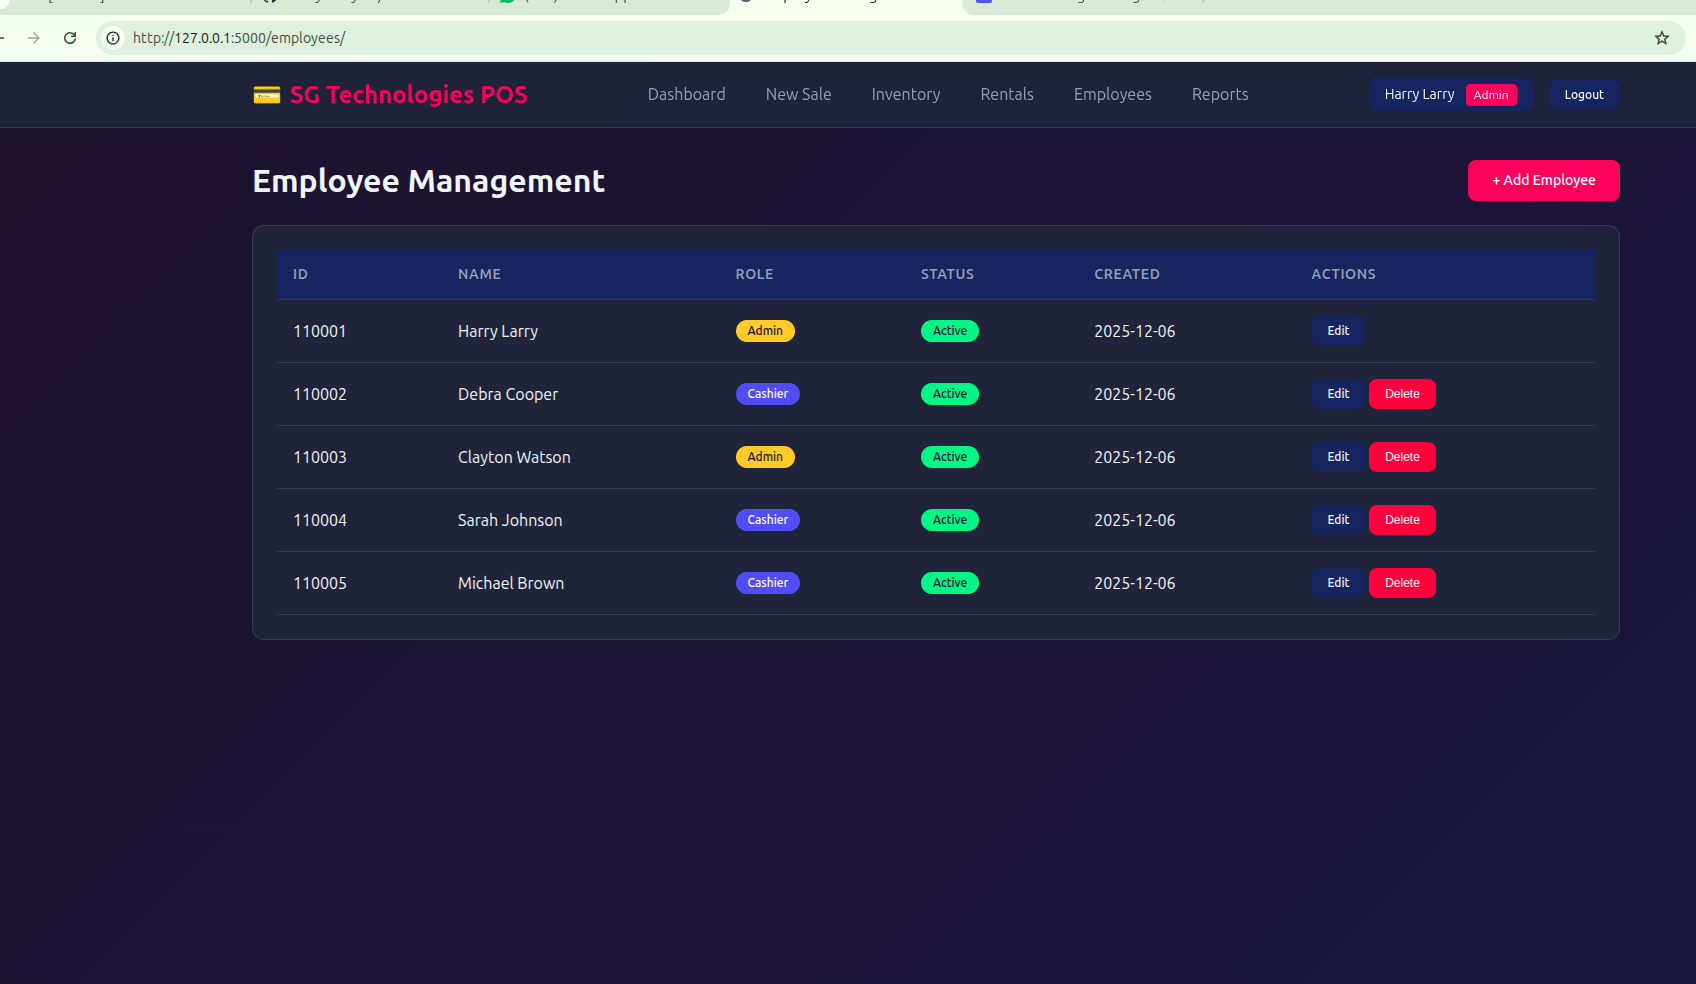
\includegraphics[width=0.95\textwidth]{images/6.png}
  \caption{Employee Management Interface -- Migrated employee data now includes
           unique IDs, role badges (Admin/Cashier), status indicators, creation
           timestamps, and action buttons. Passwords are securely hashed.}
  \label{fig:employee-management}
\end{figure}

\begin{figure}[h]
  \centering
  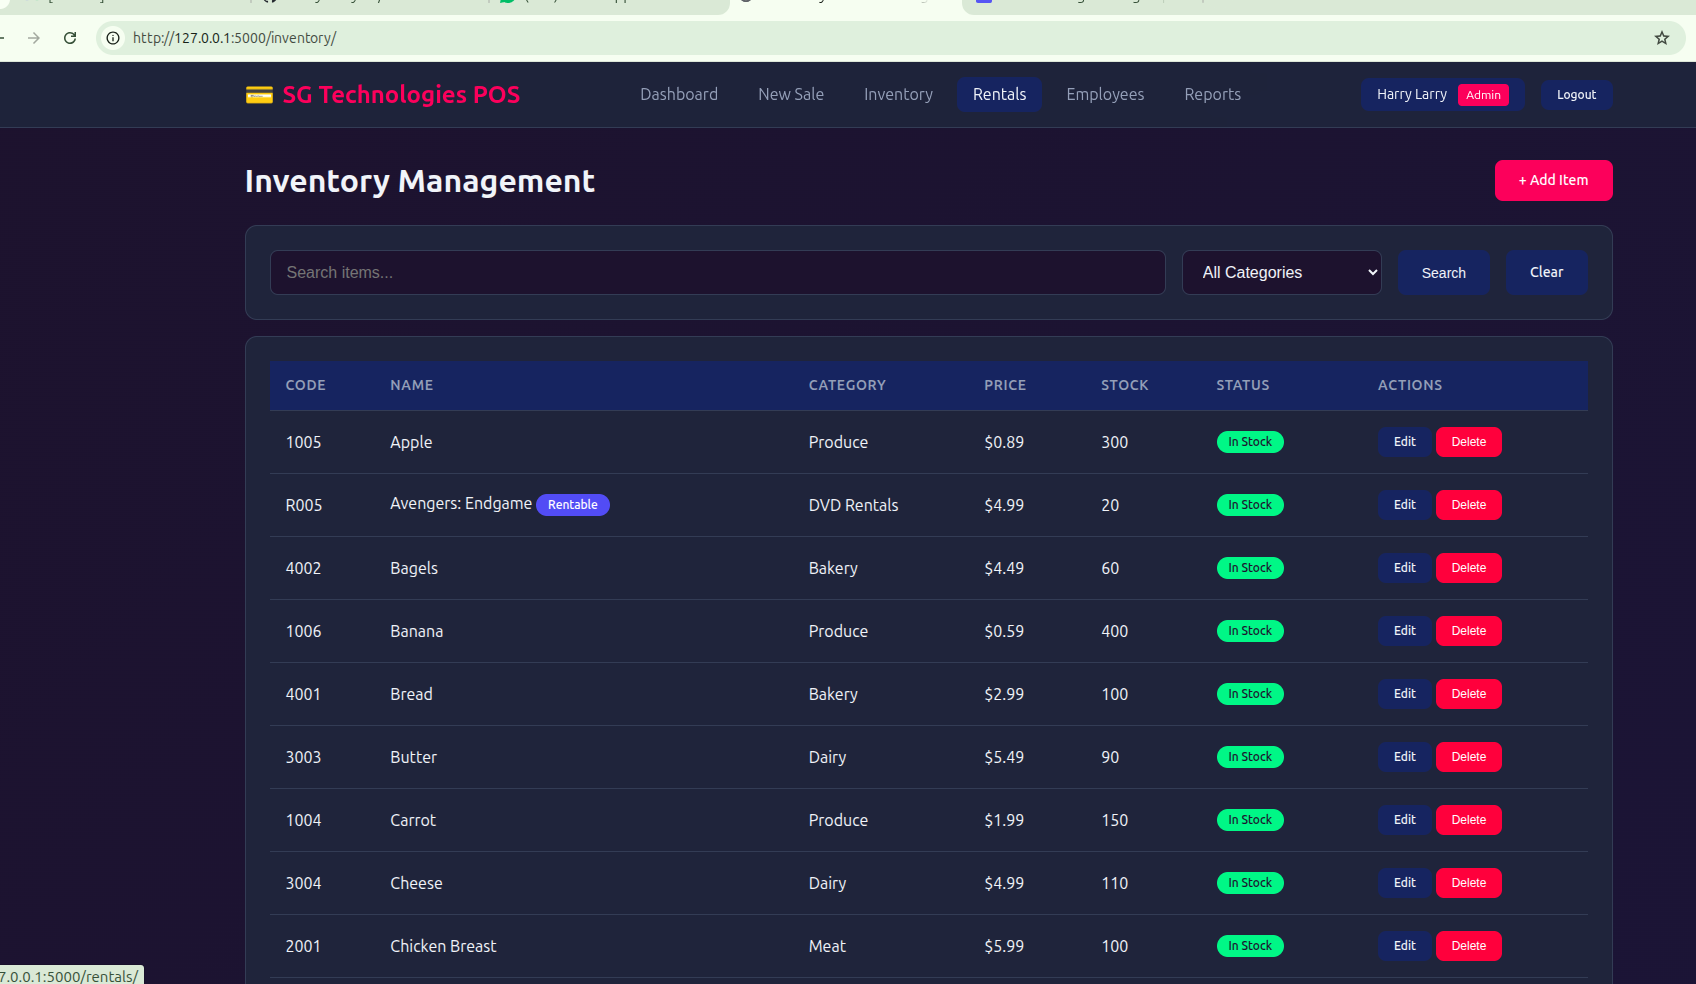
\includegraphics[width=0.95\textwidth]{images/3.png}
  \caption{Inventory Management Interface -- Migrated item data with proper
           categories (Produce, Bakery, Dairy, Meat, DVD Rentals), prices,
           stock quantities, status indicators, and the new ``Rentable'' badge
           for items that can be rented.}
  \label{fig:inventory-management}
\end{figure}

%=================================================
\chapter{Forward Engineering Report (Point 5)}
%=================================================

This chapter documents the forward engineering process for transforming
the legacy Java desktop POS system into a modern web-based application.

\section{Executive Summary}

Key achievements of the reengineered system:

\begin{itemize}[leftmargin=1.2cm]
  \item Transformed from a desktop Java Swing application to a
        web-based architecture.
  \item Migrated from legacy \texttt{.txt} files to a normalised
        SQLite/PostgreSQL database.
  \item Implemented secure password hashing instead of plain-text
        credentials.
  \item Introduced a proper layered architecture (MVC + Service Layer).
  \item Implemented comprehensive audit logging.
  \item Added a modern, responsive web UI.
  \item Achieved comprehensive automated test coverage on critical
        components.
\end{itemize}

\begin{figure}[h]
  \centering
  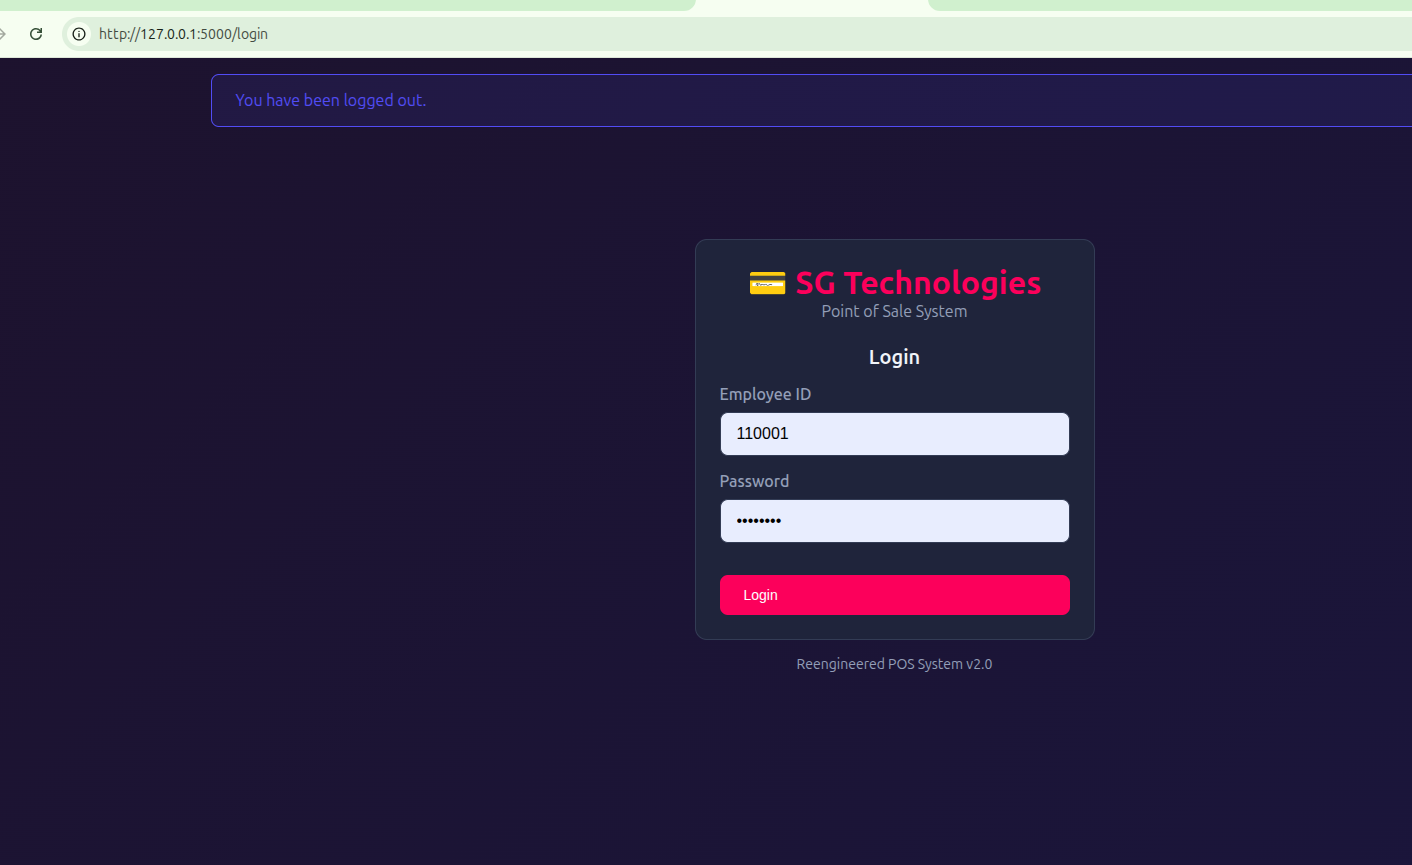
\includegraphics[width=0.85\textwidth]{images/1.png}
  \caption{Reengineered Login Interface -- Modern, responsive design with
           secure authentication. Employee ID and password are validated
           against the database with hashed password comparison.}
  \label{fig:login-interface}
\end{figure}

\section{Technology Stack Selection}

\subsection{Programming Language: Python 3.x}

Python was selected as the primary implementation language because of:

\begin{itemize}[leftmargin=1.2cm]
  \item Clean, readable syntax that improves maintainability.
  \item Rapid development cycle and rich ecosystem for web development.
  \item Large community support and extensive libraries.
\end{itemize}

\begin{table}[h]
  \centering
  \caption{Legacy vs Reengineered Language Choice}
  \begin{tabular}{p{3cm} p{4.5cm} p{4.5cm}}
    \toprule
    \textbf{Aspect} & \textbf{Legacy (Java)} & \textbf{Reengineered (Python)} \\
    \midrule
    Lines of Code & $\sim 2500$ & $\sim 1800$ \\
    Setup Time    & Complex (JDK, IDE, classpath) & Simple (\texttt{pip install}) \\
    Deployment    & JAR file                      & WSGI server \\
    Testing       & JUnit                         & Pytest (simpler, lightweight) \\
    \bottomrule
  \end{tabular}
\end{table}

\subsection{Web Framework: Flask}

Flask was chosen as the web framework due to:

\begin{itemize}[leftmargin=1.2cm]
  \item Lightweight core with minimal overhead.
  \item High flexibility, allowing architecture to be customised.
  \item Blueprint support for modular route organisation.
  \item Rich extension ecosystem (Flask-SQLAlchemy, Flask-Login, etc.).
\end{itemize}

\subsection{Database: SQLite / PostgreSQL}

\begin{table}[h]
  \centering
  \caption{Legacy Text Files vs Relational Database}
  \begin{tabular}{p{3cm} p{4.5cm} p{4.5cm}}
    \toprule
    \textbf{Feature} & \textbf{\texttt{.txt} Files} & \textbf{Relational DB} \\
    \midrule
    Data Integrity    & None                 & Constraints, types, keys \\
    Concurrent Access & File locks           & ACID transactions \\
    Query Capability  & Parse entire file    & SQL queries \\
    Relationships     & Embedded / duplicated & Foreign keys \\
    Scalability       & Poor                 & Excellent \\
    \bottomrule
  \end{tabular}
\end{table}

\section{Architecture Design}

\subsection{Layered Architecture + MVC}

\begin{figure}[h]
  \centering
  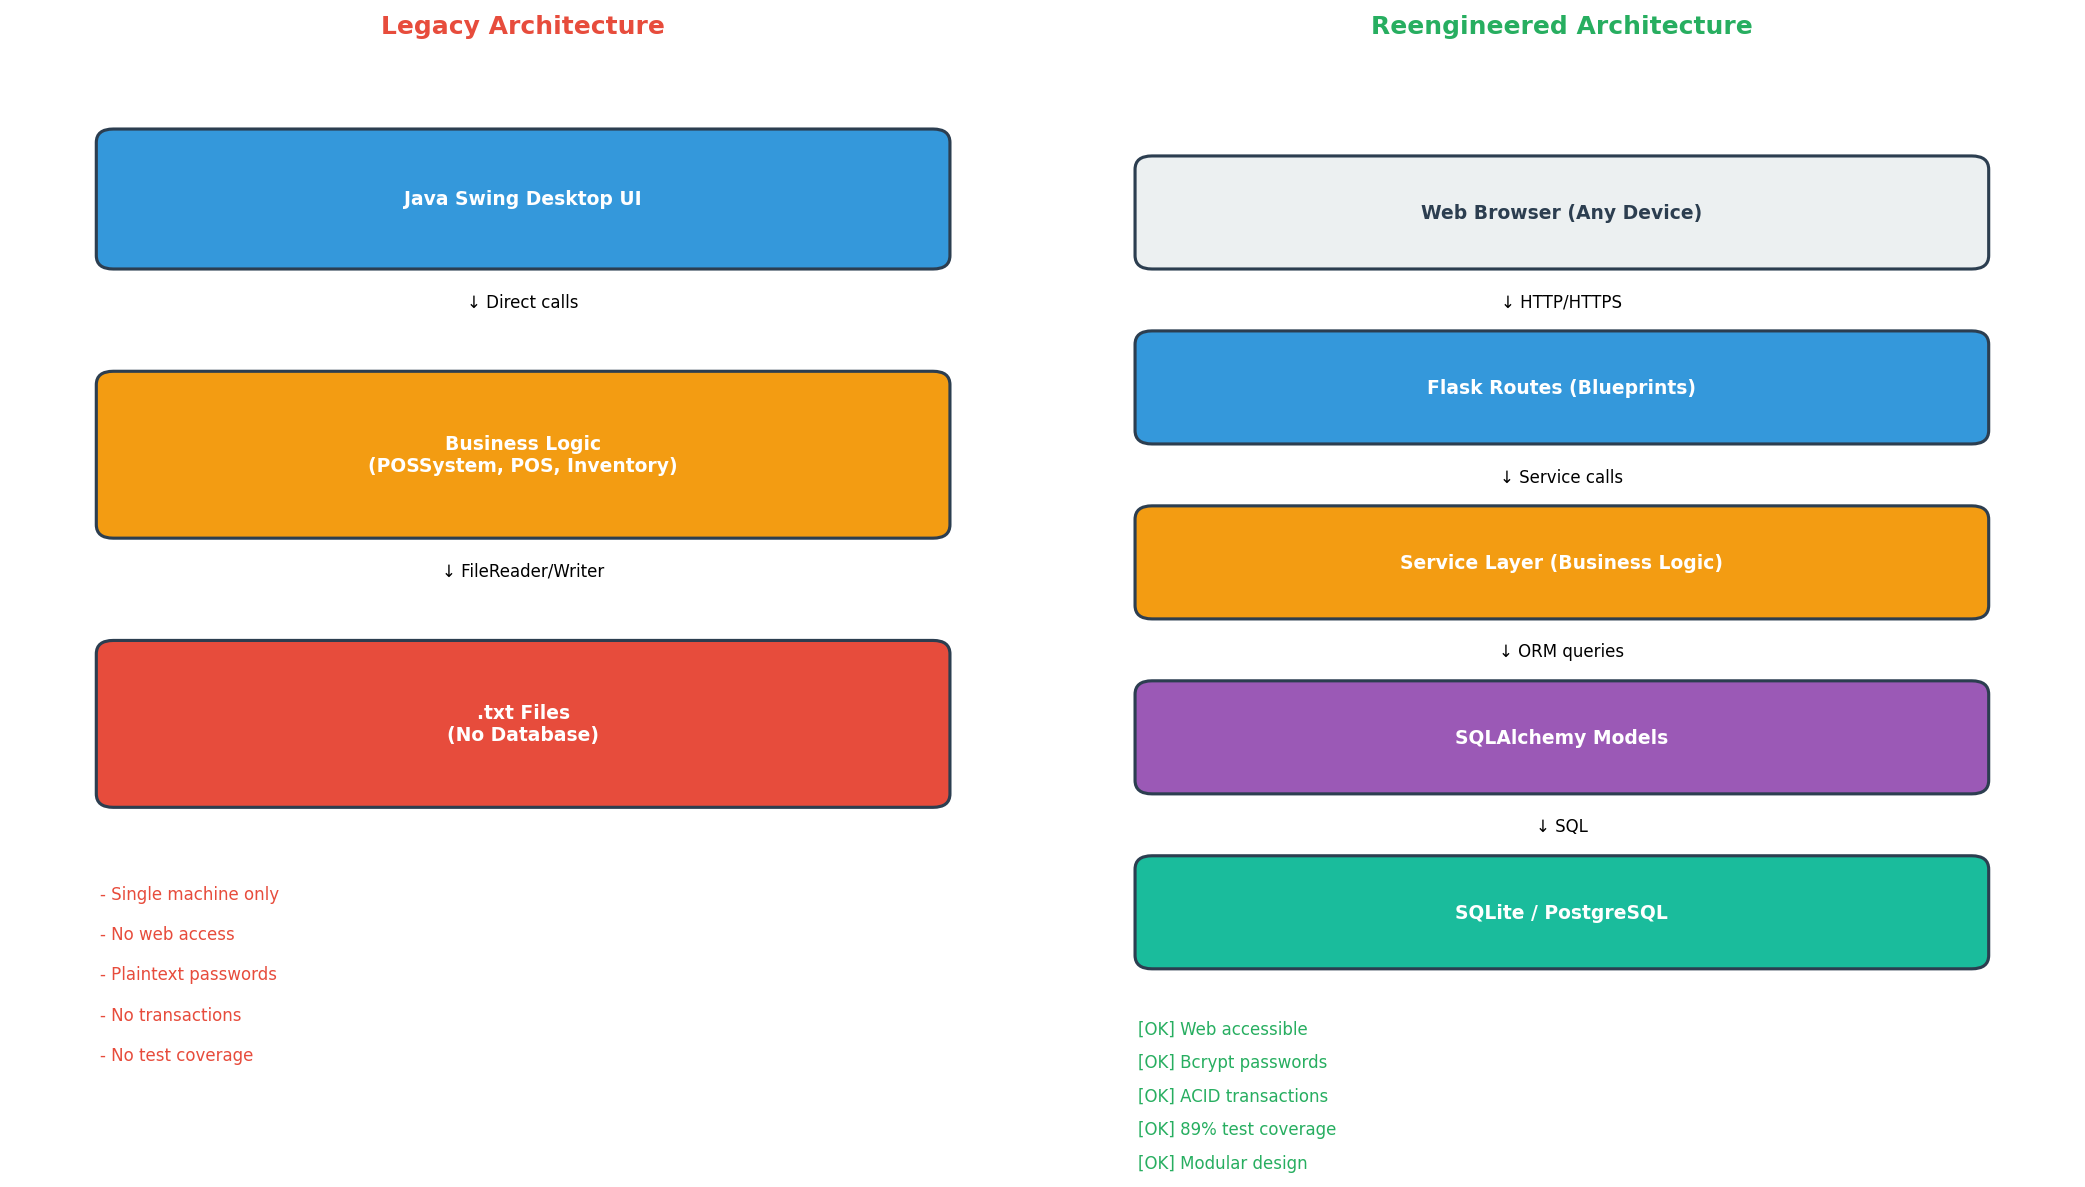
\includegraphics[width=0.95\textwidth]{images/architecture_comparison.png}
  \caption{Architecture Comparison -- Legacy monolithic Java Swing application (left)
           vs Reengineered layered Flask web application (right). The new architecture
           demonstrates clear separation of concerns with distinct Presentation,
           Business Logic, Data Access, and Database layers.}
  \label{fig:architecture-comparison}
\end{figure}

\begin{table}[h]
  \centering
  \caption{Architecture Layers}
  \begin{tabular}{p{3cm} p{4cm} p{5cm}}
    \toprule
    \textbf{Layer} & \textbf{Components} & \textbf{Responsibility} \\
    \midrule
    Presentation &
      Routes (Flask Blueprints), Templates (Jinja2), Static Assets &
      User interface and HTTP handling \\
    Business Logic &
      \texttt{AuthService}, \texttt{SalesService},
      \texttt{InventoryService}, \texttt{RentalService} &
      Core business rules \\
    Data Access &
      Models: \texttt{Employee}, \texttt{Item}, \texttt{Sale},
      \texttt{Rental}, \texttt{ActivityLog} &
      Database operations \\
    Database &
      SQLite / PostgreSQL &
      Data persistence \\
    \bottomrule
  \end{tabular}
\end{table}

\section{Design Patterns Used}

\begin{table}[h]
  \centering
  \caption{Design Patterns in the Reengineered System}
  \begin{tabular}{p{3cm} p{5cm} p{4cm}}
    \toprule
    \textbf{Pattern} & \textbf{Implementation} & \textbf{Benefit} \\
    \midrule
    MVC &
      Flask Blueprints + Jinja2 Templates + Models &
      Separation of concerns \\
    Repository &
      SQLAlchemy Models &
      Data access abstraction \\
    Service Layer &
      \texttt{app/services/} &
      Centralised business logic \\
    Factory &
      \texttt{create\_app()} in \texttt{\_\_init\_\_.py} &
      Configurable app creation \\
    Singleton &
      Flask extensions (\texttt{db}, \texttt{login\_manager}) &
      Single instance per app context \\
    Blueprint &
      Route modules under \texttt{app/routes/} &
      Modular code organisation \\
    \bottomrule
  \end{tabular}
\end{table}

\section{Component Mapping}

\begin{table}[h]
  \centering
  \caption{Legacy to Reengineered Component Mapping}
  \begin{tabular}{p{4cm} p{5cm} p{4cm}}
    \toprule
    \textbf{Legacy Component} & \textbf{Reengineered Component} & \textbf{Improvements} \\
    \midrule
    \texttt{Login\_Interface.java} &
      \texttt{routes/auth.py}, templates under \texttt{templates/auth/} &
      Session-based auth, secure passwords \\
    \texttt{Employee.java} &
      \texttt{models/employee.py} &
      Password hashing, relationships \\
    \texttt{Item.java} &
      \texttt{models/item.py} &
      Stock tracking, categories \\
    \texttt{POS.java} &
      \texttt{services/sales\_service.py} &
      Transaction management \\
    \texttt{.txt} files &
      SQLite/PostgreSQL &
      ACID-compliant persistence \\
    \bottomrule
  \end{tabular}
\end{table}

\section{User Interface Screenshots}

The following screenshots demonstrate the reengineered system's modern web interface,
showcasing the implementation of all major functional areas.

\subsection{Role-Based Dashboards}

\begin{figure}[h]
  \centering
  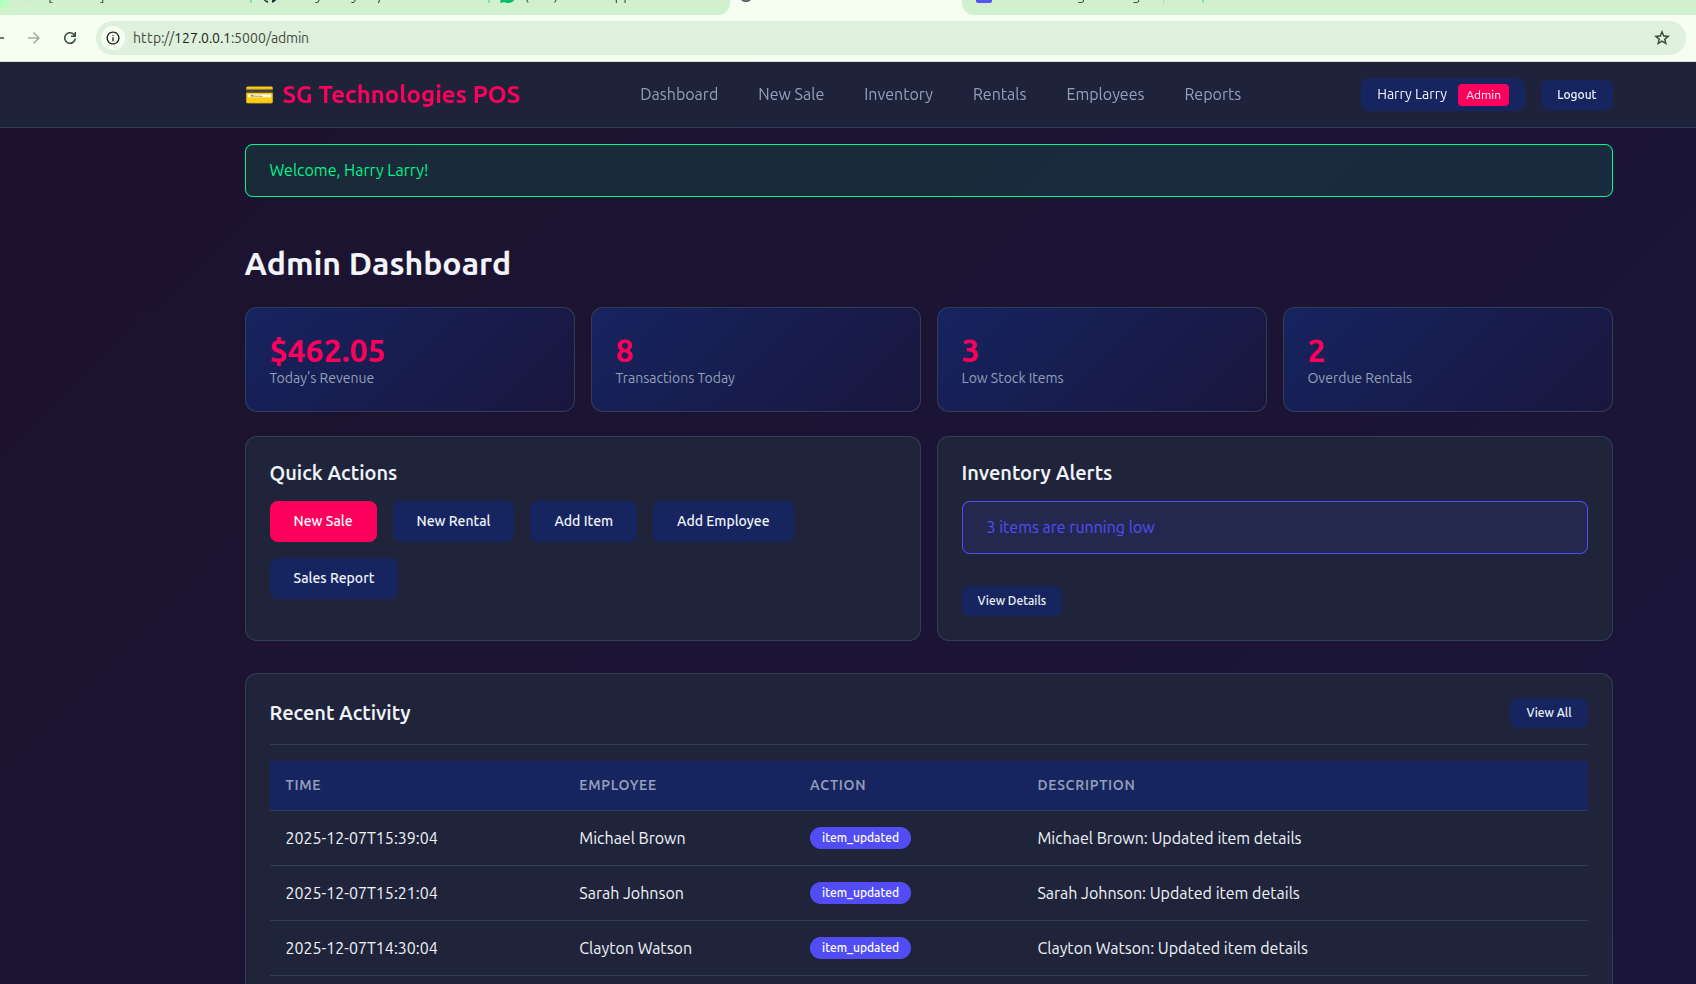
\includegraphics[width=0.95\textwidth]{images/2.png}
  \caption{Admin Dashboard -- Displays today's revenue (\$462.05), transaction count,
           low stock items (3), and overdue rentals (2). Quick actions allow admins
           to create sales, rentals, add items, and add employees. Recent activity
           log shows audit trail of all system actions.}
  \label{fig:admin-dashboard}
\end{figure}

\begin{figure}[h]
  \centering
  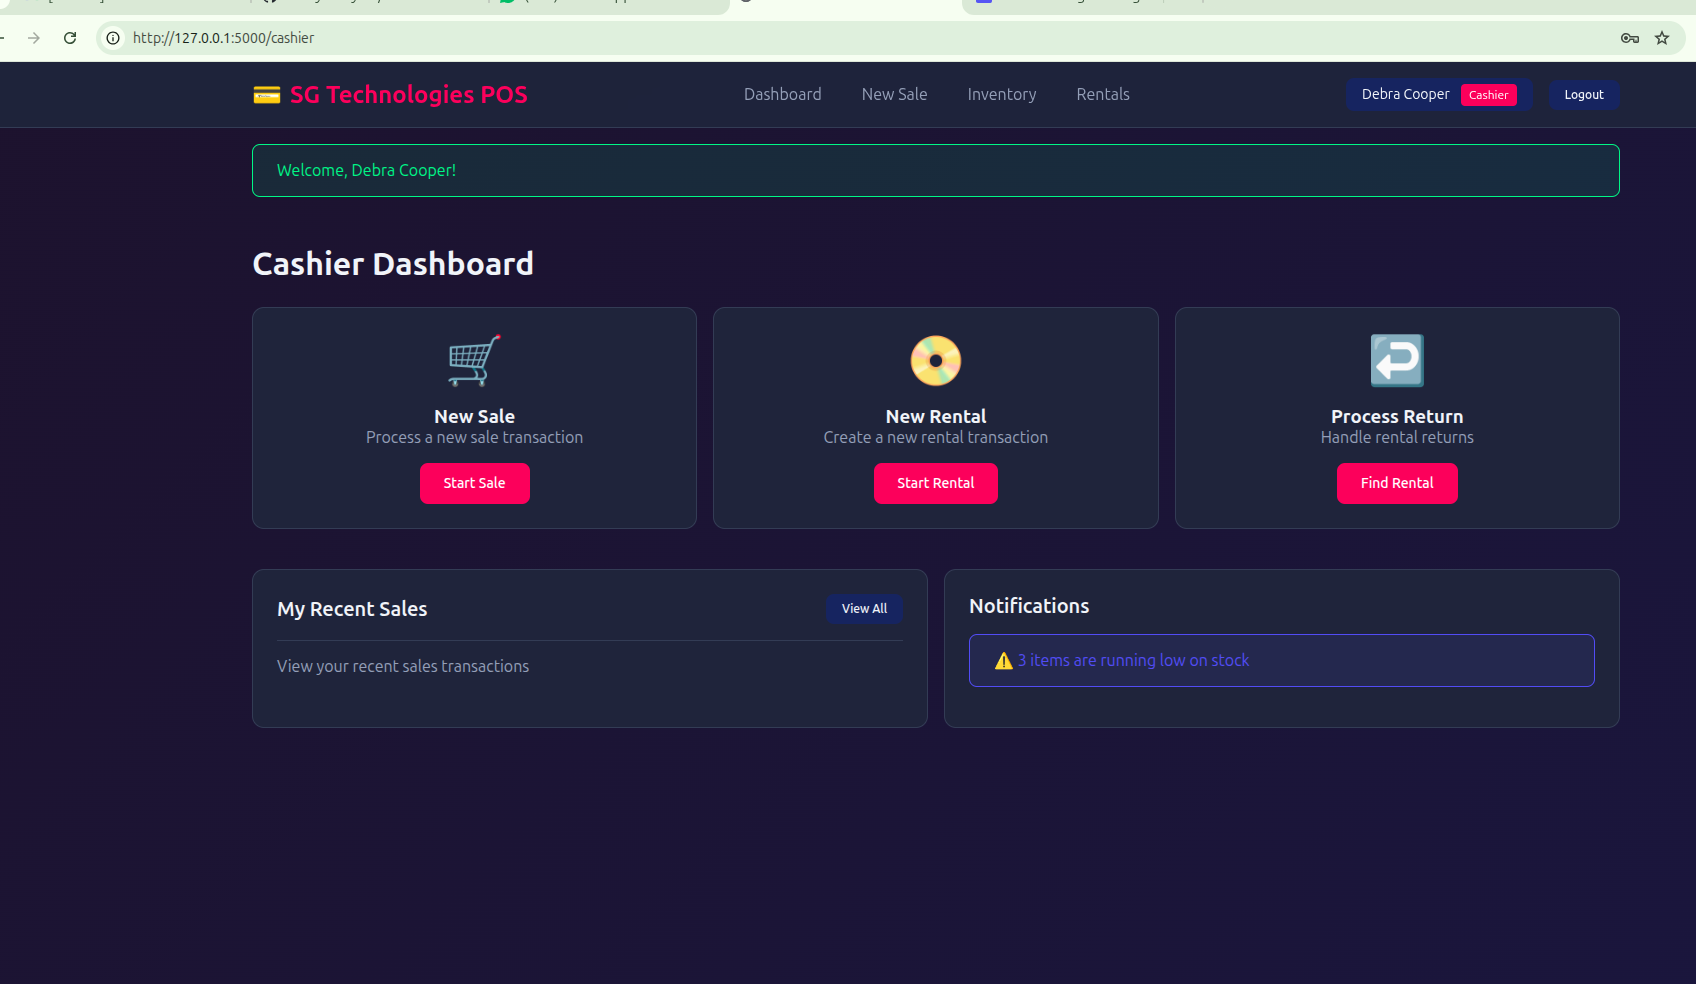
\includegraphics[width=0.95\textwidth]{images/7.png}
  \caption{Cashier Dashboard -- Simplified interface for cashier role with quick
           access to New Sale, New Rental, and Process Return functions. Shows
           notifications for low stock items and recent sales history.}
  \label{fig:cashier-dashboard}
\end{figure}

\subsection{Point of Sale Interface}

\begin{figure}[h]
  \centering
  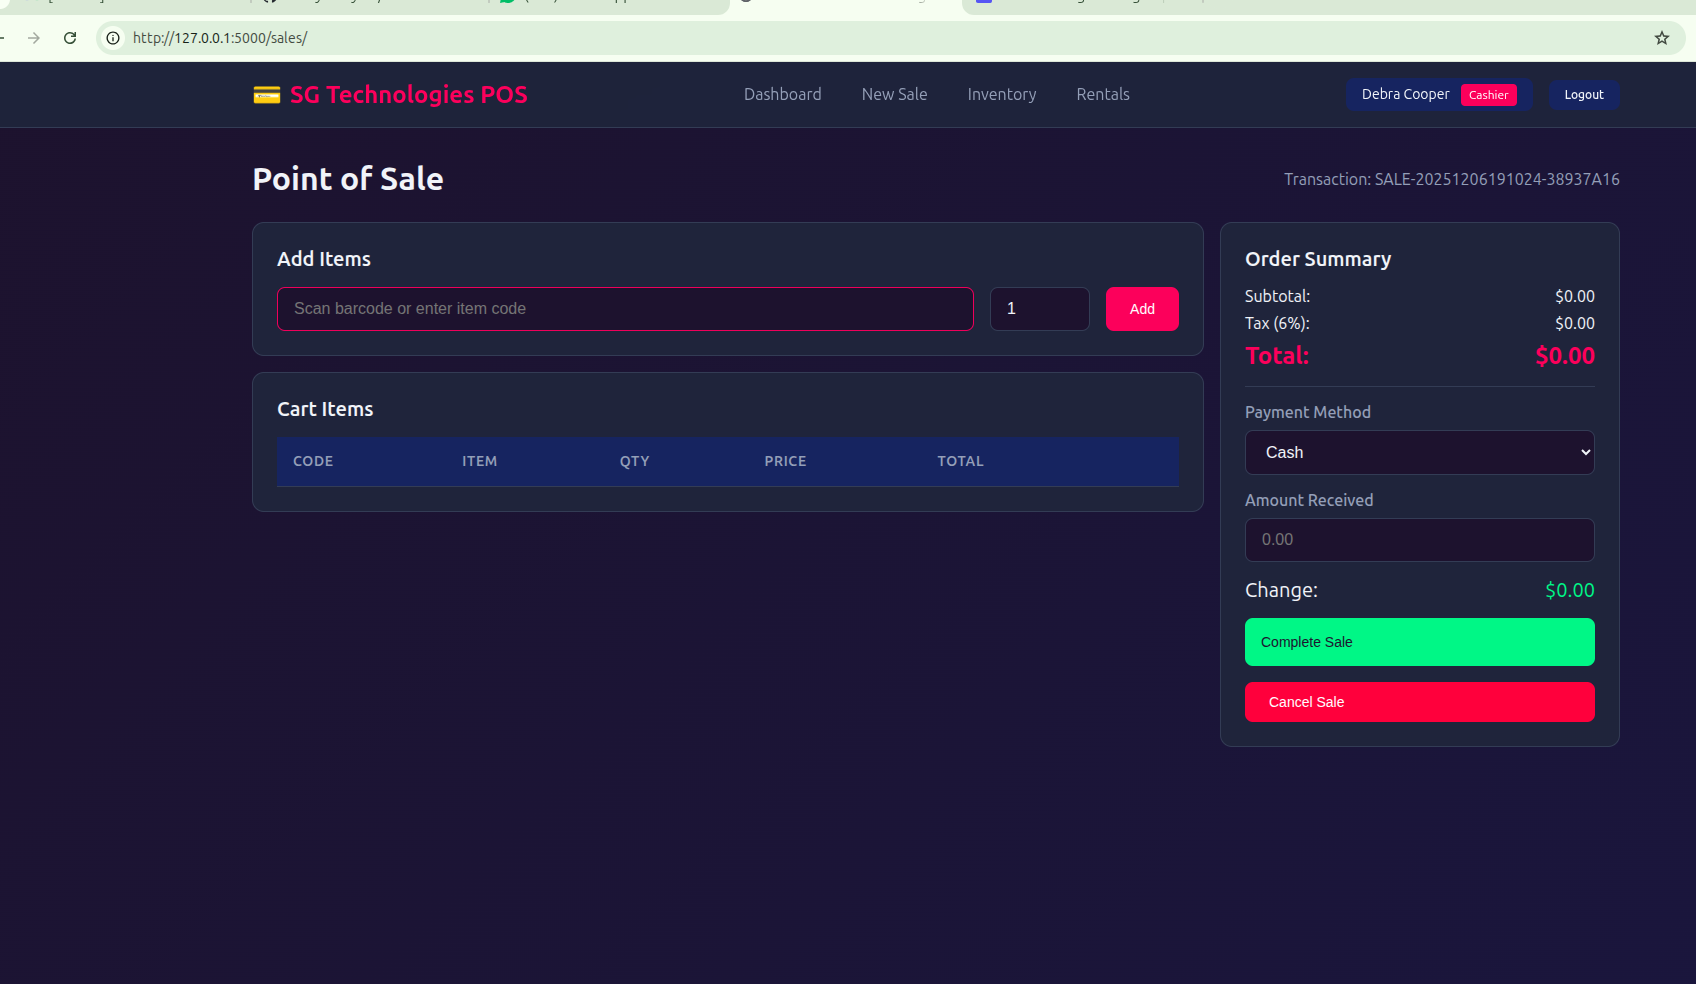
\includegraphics[width=0.95\textwidth]{images/8.png}
  \caption{Point of Sale Interface -- Modern cart-based sales system with barcode/item
           code entry, real-time order summary showing subtotal, tax (6\%), and total.
           Payment method selection (Cash) with change calculation and Complete/Cancel
           buttons.}
  \label{fig:pos-interface}
\end{figure}

\subsection{Rental Management}

\begin{figure}[h]
  \centering
  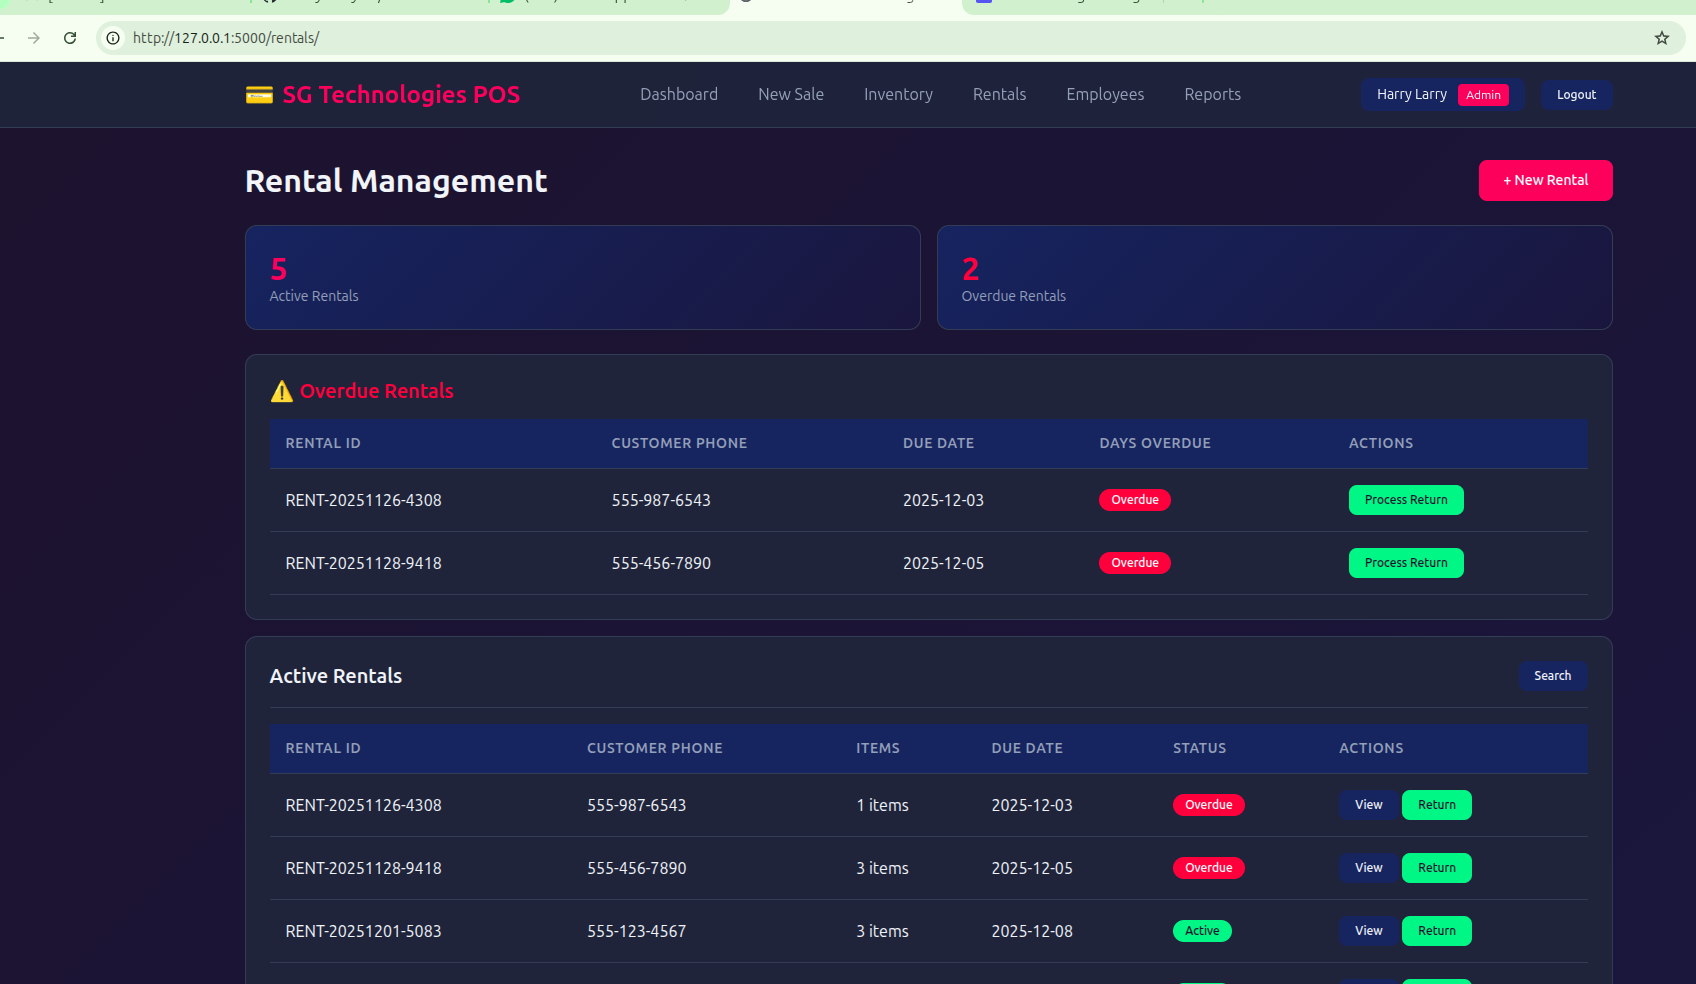
\includegraphics[width=0.95\textwidth]{images/4.png}
  \caption{Rental Management Interface -- Shows active rentals (5) and overdue rentals
           (2) with customer phone, due dates, and status indicators. Includes ``Process
           Return'' and ``View'' actions for each rental transaction.}
  \label{fig:rental-management}
\end{figure}

\subsection{Reports Dashboard}

\begin{figure}[h]
  \centering
  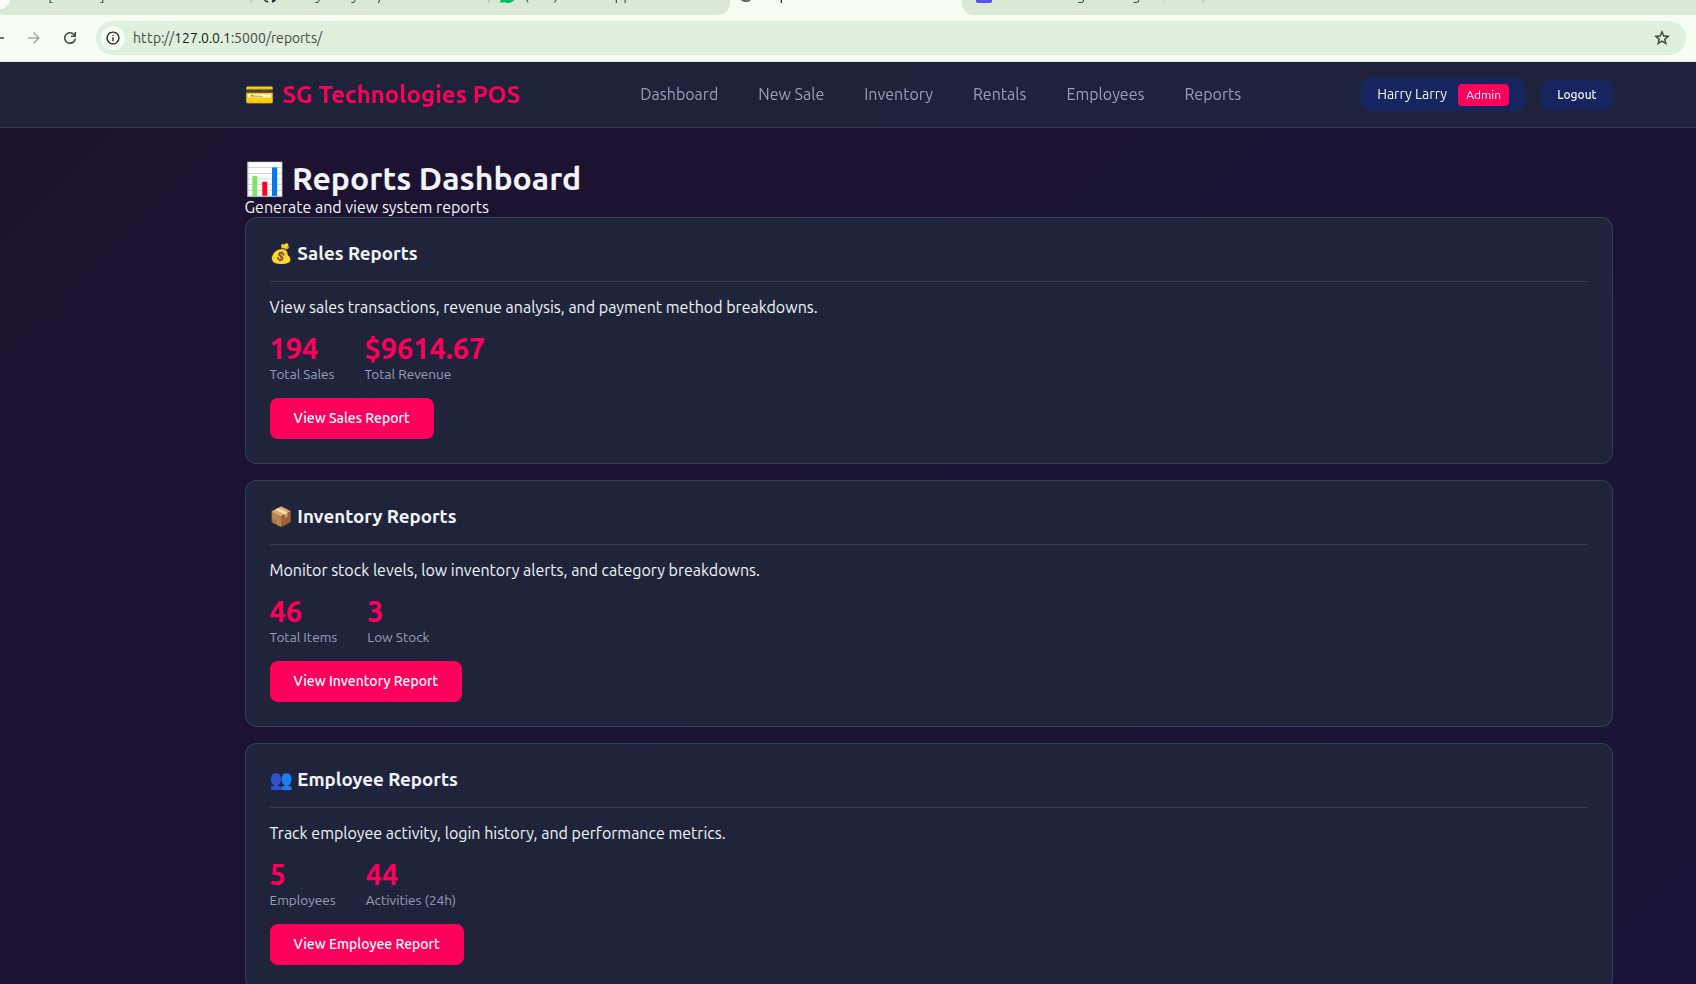
\includegraphics[width=0.95\textwidth]{images/5.png}
  \caption{Reports Dashboard -- Comprehensive reporting with Sales Reports (194 total
           sales, \$9614.67 revenue), Inventory Reports (46 items, 3 low stock), and
           Employee Reports (5 employees, 44 activities in 24h).}
  \label{fig:reports-dashboard}
\end{figure}

\section{Deployment Guide}

\subsection{Development Setup}

\begin{enumerate}[leftmargin=1.2cm]
  \item Navigate to reengineered directory: \texttt{cd reengineered}
  \item Create virtual environment: \texttt{python -m venv venv}
  \item Activate virtual environment: \texttt{source venv/bin/activate}
  \item Install dependencies: \texttt{pip install -r requirements.txt}
  \item Run development server: \texttt{python run.py}
  \item Access the app at \url{http://127.0.0.1:5000}
\end{enumerate}

\subsubsection*{Default Login Credentials}

\begin{itemize}[leftmargin=1.2cm]
  \item Admin: \texttt{110001 / admin123}
  \item Cashier: \texttt{110002 / cashier123}
\end{itemize}

%=================================================
\chapter{Reengineering Plan and Migration (Point 6)}
%=================================================

\section{Objectives}

The goal of this reengineering plan is to transform the legacy Java desktop--based
Point-of-Sale (POS) system, which relies on plain text (\texttt{.txt}) files for
persistence, into a modern, web-based architecture with a normalized relational
database backend.

This plan covers:
\begin{itemize}
  \item The phased reengineering approach from inventory analysis to forward engineering.
  \item A realistic timeline with milestones and responsibilities.
  \item The end-to-end data migration strategy from text files to a relational database.
  \item Risk-aware execution, aligned with the risk analysis and testing strategy.
\end{itemize}

\section{Reengineering Process Flow}

Figure~\ref{fig:reengineering-flow} illustrates the complete reengineering
process from legacy system analysis to the delivery of the modernized web
application.

\begin{figure}[h]
  \centering
  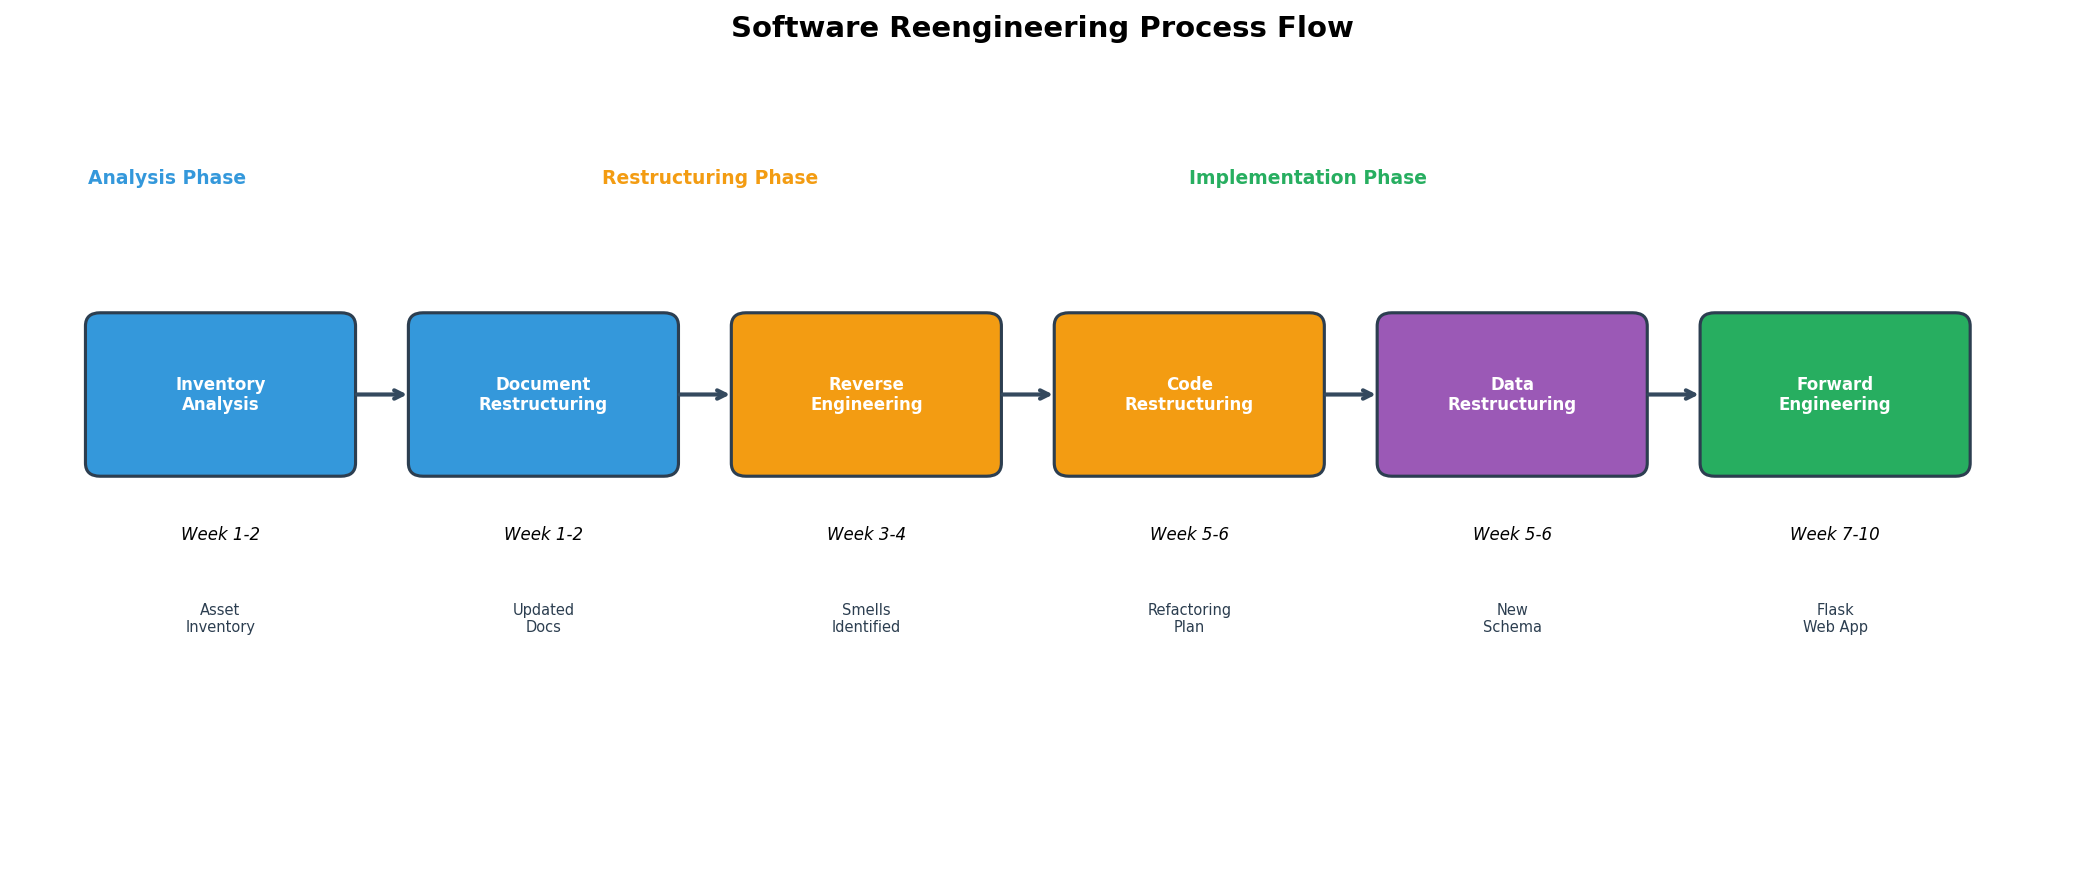
\includegraphics[width=0.95\textwidth]{images/reengineering_flow.png}
  \caption{Software Reengineering Process Flow -- The systematic transformation
           from legacy Java desktop POS system to modern Flask web application,
           following all phases of the reengineering model.}
  \label{fig:reengineering-flow}
\end{figure}

\section{Phase Overview}

\begin{table}[h]
  \centering
  \caption{Reengineering Phases Overview}
  \begin{tabular}{p{3.2cm} p{10.0cm}}
    \toprule
    \textbf{Phase} & \textbf{Description} \\
    \midrule
    Inventory Analysis &
      Identify and classify all legacy assets (Java source files, libraries,
      configuration files, and text-based ``database'' files). \\
    Document Restructuring &
      Reconstruct and reorganize technical documentation to reflect the actual
      structure, modules, and data flows. \\
    Reverse Engineering &
      Analyze the legacy codebase to recover design, workflows, and data
      structures. Identify code smells and data smells. \\
    Code Restructuring &
      Propose and apply refactorings to improve modularity, readability,
      and separation of concerns. \\
    Data Restructuring &
      Redesign the data model as a normalized relational schema (3NF),
      define table structures and constraints. \\
    Forward Engineering &
      Implement the reengineered POS system as a web-based application. \\
    \bottomrule
  \end{tabular}
\end{table}

\section{Timeline and Milestones}

\begin{table}[h]
  \centering
  \caption{High-Level Reengineering Timeline}
  \begin{tabular}{p{2.2cm} p{10.0cm}}
    \toprule
    \textbf{Weeks} & \textbf{Planned Activities and Milestones} \\
    \midrule
    Week 1--2 &
      \textbf{Inventory Analysis \& Document Restructuring} --
      Collect all legacy artefacts, build asset inventory and dependency map. \\
    Week 3--4 &
      \textbf{Reverse Engineering \& Smell Detection} --
      Recover workflows, identify code and data smells. \\
    Week 5--6 &
      \textbf{Code Restructuring \& Data Restructuring Design} --
      Define repository and service abstractions, design normalized schema. \\
    Week 7--8 &
      \textbf{Forward Engineering (Web Architecture)} --
      Implement Flask application structure (models, services, routes). \\
    Week 9 &
      \textbf{Data Migration Implementation \& Dry Runs} --
      Implement migration script, execute dry runs, verify record counts. \\
    Week 10 &
      \textbf{Testing, Risk Mitigation \& Finalization} --
      Execute automated tests, validate risk mitigations, complete documentation. \\
    \bottomrule
  \end{tabular}
\end{table}

\section{Risk Considerations}

The reengineering plan explicitly addresses potential risks at each phase.
Table~\ref{tab:phase-risks} summarizes the key risks and their mitigation
strategies integrated into the timeline.

\begin{table}[h]
  \centering
  \caption{Risk Considerations by Phase}
  \label{tab:phase-risks}
  \begin{tabular}{p{3.5cm} p{4.5cm} p{5cm}}
    \toprule
    \textbf{Phase} & \textbf{Key Risk} & \textbf{Mitigation Strategy} \\
    \midrule
    Inventory Analysis &
      Incomplete asset identification &
      Systematic directory scan; cross-reference with documentation \\
    Reverse Engineering &
      Misunderstanding legacy workflows &
      Trace execution paths; validate with sample transactions \\
    Code Restructuring &
      Breaking existing functionality &
      Incremental refactoring; regression testing after each change \\
    Data Restructuring &
      Data loss during schema migration &
      Full backup before migration; staged migration with validation \\
    Forward Engineering &
      Architecture drift from design &
      Code reviews; adherence to layered architecture patterns \\
    Migration Execution &
      Production data corruption &
      Dry runs on test data; rollback scripts prepared \\
    \bottomrule
  \end{tabular}
\end{table}

\subsection{Critical Risk Mitigation}

The following high-priority risks are addressed throughout the plan:

\begin{itemize}
  \item \textbf{R1 -- Data Loss:} Mandatory backup of all \texttt{.txt} files before
        any migration; record count verification at each stage.
  \item \textbf{R2 -- Authentication Security:} Passwords are hashed during the
        Transform phase; plaintext passwords are never stored in the new database.
  \item \textbf{R3 -- Functional Regression:} All original POS functionality
        (sales, rentals, returns, inventory) is verified through automated tests
        before deployment.
  \item \textbf{R4 -- Timeline Overrun:} Buffer time allocated in Weeks 9--10 for
        unexpected issues; phased approach allows for incremental delivery.
\end{itemize}

\section{Migration Strategy}

\subsection{Migration Objectives}

\begin{itemize}
  \item Preserve \textbf{100\%} of valid legacy data from text files.
  \item Eliminate structural, security, and quality smells via normalization.
  \item Ensure that migration is \emph{idempotent} and \emph{verifiable}
        through record counts and integrity checks.
\end{itemize}

\subsection{Migration Phases}

\begin{table}[h]
  \centering
  \caption{Data Migration Phases}
  \begin{tabular}{p{3.0cm} p{9.7cm}}
    \toprule
    \textbf{Phase} & \textbf{Description} \\
    \midrule
    Backup &
      Copy all legacy \texttt{Database/} files to a timestamped backup folder. \\
    Parse &
      Read and parse legacy text files, converting each line into structured
      in-memory objects. \\
    Transform &
      Map parsed records to the new relational schema: normalize repeated groups,
      convert date formats, hash passwords. \\
    Validate &
      Perform integrity checks before committing: verify counts, ensure no
      missing mandatory fields. \\
    Load &
      Insert transformed data into the database using SQLAlchemy models. \\
    Verify &
      Run post-migration verification queries: compare record counts, check for
      orphan records. \\
    \bottomrule
  \end{tabular}
\end{table}

\section{Roles and Responsibilities}

\begin{table}[h]
  \centering
  \caption{Roles and Responsibilities Across Phases}
  \begin{tabular}{p{4.5cm} p{3.2cm} p{5.0cm}}
    \toprule
    \textbf{Member} & \textbf{Primary Phases} & \textbf{Key Responsibilities} \\
    \midrule
    Abdul Faheem (22i--2629) &
      Inventory, Reverse Engineering &
      Asset inventory and dependency mapping; legacy workflow analysis;
      identification of code/data smells; initial legacy documentation. \\
    Sheryar Ali (22i--2623) &
      Code Restructuring, Data Restructuring &
      Refactoring proposals; design of the normalized relational schema;
      specification of migration rules and mapping. \\
    Husnain Akram (22i--2464) &
      Forward Engineering, Testing, Migration &
      Implementation of the Flask-based web architecture; migration scripts;
      automated tests and risk mitigation activities. \\
    \bottomrule
  \end{tabular}
\end{table}

\section{Deliverables and Exit Criteria}

The reengineering and migration effort is considered complete when:

\begin{itemize}
  \item The normalized relational schema is implemented and documented.
  \item All relevant legacy data has been successfully migrated with
        verified record counts and integrity checks.
  \item The Flask-based POS application supports the original functional
        requirements (sales, rentals, inventory, employee management).
  \item Automated tests (models, services, routes) pass with the targeted
        coverage level and are repeatable via the project test suite.
  \item Risk mitigations for data loss, authentication, SQL injection,
        and concurrency are in place and documented.
  \item Dual documentation (legacy vs reengineered) and the signed
        work-distribution table are finalized.
\end{itemize}

%=================================================
\chapter{Refactoring Documentation (Point 7)}
%=================================================

This chapter documents individual refactorings contributed by each team
member. Each refactoring includes the context, before/after code,
rationale, and impact on quality attributes.

Each team member has performed and documented at least \textbf{three major
refactorings} as required by the project rubric. The refactorings are
categorized by type and include measurable quality impacts.

\begin{figure}[h]
  \centering
  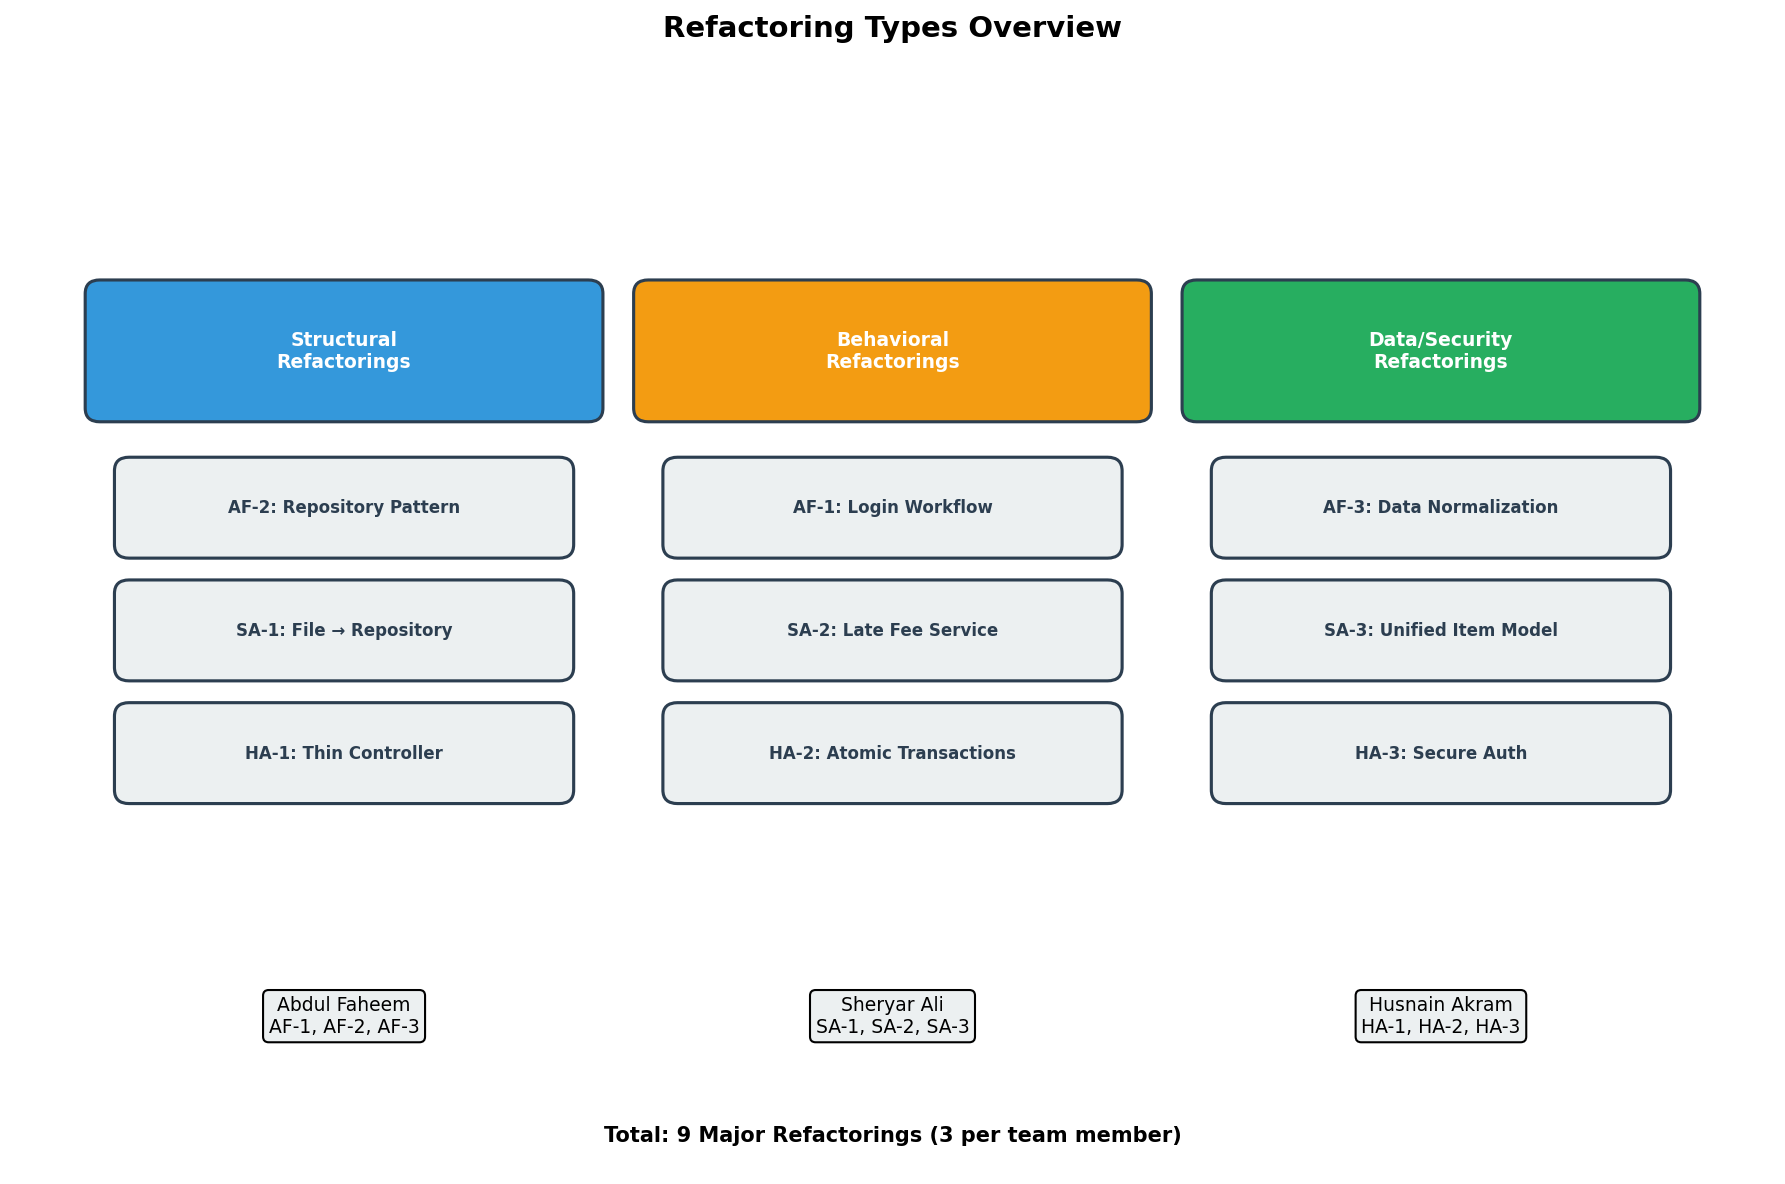
\includegraphics[width=0.95\textwidth]{images/refactoring_overview.png}
  \caption{Overview of Refactoring Types -- Distribution of refactorings across
           structural, behavioral, and data categories by team member.}
  \label{fig:refactoring-overview}
\end{figure}

\section{Refactoring Summary}

\begin{table}[h]
  \centering
  \caption{Summary of Individual Refactorings}
  \begin{tabular}{p{3.5cm} p{1.5cm} p{4cm} p{4cm}}
    \toprule
    \textbf{Member} & \textbf{ID} & \textbf{Refactoring} & \textbf{Type} \\
    \midrule
    Abdul Faheem & AF--1 & Login Workflow Clarification & Behavioral \\
    (22i--2629)  & AF--2 & Repository Abstraction & Structural \\
                 & AF--3 & Data Normalization (1NF) & Data \\
    \midrule
    Sheryar Ali  & SA--1 & File Write to Repository & Structural \\
    (22i--2623)  & SA--2 & Late-Fee Service Extraction & Behavioral \\
                 & SA--3 & Unified Item Model & Data \\
    \midrule
    Husnain Akram & HA--1 & Thin Controller Pattern & Structural \\
    (22i--2464)   & HA--2 & Atomic Transaction Service & Behavioral \\
                  & HA--3 & Secure Authentication & Security \\
    \bottomrule
  \end{tabular}
\end{table}

%=========================================================
\section{Abdul Faheem (22i--2629)}
%=========================================================

\subsection{AF--1: Clarify Login Workflow with Explicit Role Check}

\textbf{Context:}
The legacy \texttt{Login\_Interface.java} directly called
\texttt{POSSystem.logIn(...)} and relied on implicit global state to
determine which UI to show next (Cashier vs Admin).

\textbf{Before (Legacy Java):}
\begin{lstlisting}[language=Java]
// Login_Interface.java
if (POSSystem.logIn(username, password)) {
    // role determined by global POSSystem.role
    if (POSSystem.role.equals("Admin")) {
        new Admin_Interface();
    } else {
        new Cashier_Interface();
    }
}
\end{lstlisting}

\textbf{After (Reengineered Python/Flask):}
\begin{lstlisting}[language=Python]
# routes/auth.py
@auth_bp.route('/login', methods=['POST'])
def login():
    success, employee, message = AuthService.authenticate(
        request.form['employee_id'],
        request.form['password']
    )
    if success:
        login_user(employee)
        if employee.role == 'Admin':
            return redirect(url_for('main.admin_dashboard'))
        return redirect(url_for('main.cashier_dashboard'))
    flash(message, 'error')
    return redirect(url_for('auth.login'))
\end{lstlisting}

\textbf{Rationale:}
Explicit role check after authentication improves readability and removes
dependence on global mutable state. The Flask-Login extension provides
secure session management, while the service layer handles credential
verification.

\textbf{Impact:}
\begin{itemize}
  \item \textbf{Coupling:} Reduced -- UI no longer depends on global state
  \item \textbf{Testability:} Improved -- \texttt{AuthService.authenticate()} can be unit tested
  \item \textbf{Security:} Enhanced -- Centralized authentication with audit logging
  \item \textbf{Complexity:} Reduced -- Single responsibility for each component
\end{itemize}

\subsection{AF--2: Introduce Repository Abstraction for Inventory Access}

\textbf{Context:}
The legacy \texttt{Inventory.java} accessed \texttt{itemDatabase.txt}
directly via \texttt{FileReader}/\texttt{BufferedReader}.

\textbf{Before (Legacy Java):}
\begin{lstlisting}[language=Java]
// Inventory.java
FileReader fr = new FileReader("Database/itemDatabase.txt");
BufferedReader br = new BufferedReader(fr);
String line;
while ((line = br.readLine()) != null) {
    // parse item
}
\end{lstlisting}

\textbf{After (Reengineered Python/Flask):}
\begin{lstlisting}[language=Python]
# services/inventory_service.py
class InventoryService:
    @staticmethod
    def get_all_items(include_inactive=False):
        query = Item.query
        if not include_inactive:
            query = query.filter_by(is_active=True)
        return query.order_by(Item.name).all()
\end{lstlisting}

\textbf{Rationale:}
Abstracting data access into a service allows the underlying storage to
change (text file to database) without impacting business logic. The ORM
provides query optimization, lazy loading, and relationship handling.

\textbf{Impact:}
\begin{itemize}
  \item \textbf{Separation of Concerns:} Data access isolated from business logic
  \item \textbf{Testability:} Service can be mocked for unit tests
  \item \textbf{Maintainability:} Database changes don't affect callers
  \item \textbf{Performance:} ORM provides query optimization and caching
\end{itemize}

\subsection{AF--3: Normalise Customer Rental Data (1NF Compliance)}

\textbf{Context:}
Legacy \texttt{userDatabase.txt} stored rental history as repeating groups
in a single line, violating first normal form.

\textbf{Before (Legacy Data):}
\begin{lstlisting}
6096515668 1000,6/30/09,true 1022,6/31/11,true
\end{lstlisting}

\textbf{After (Normalised Tables):}

\texttt{rentals} table:
\begin{lstlisting}
id | rental_id | customer_phone
1  | RENT-001  | 6096515668
\end{lstlisting}

\texttt{rental\_items} table:
\begin{lstlisting}
id | rental_id | item_id | is_returned | return_date
1  | 1         | 1000    | true        | 2009-06-30
2  | 1         | 1022    | true        | 2011-06-31
\end{lstlisting}

\textbf{Rationale:}
Normalisation eliminates repeating groups, enabling proper querying,
indexing, and referential integrity. The split into \texttt{rentals} and
\texttt{rental\_items} tables follows proper relational design.

\textbf{Impact:}
\begin{itemize}
  \item \textbf{Data Integrity:} Foreign keys enforce valid relationships
  \item \textbf{Query Capability:} SQL queries can filter, join, and aggregate
  \item \textbf{Scalability:} Database handles large datasets efficiently
  \item \textbf{Maintainability:} Clear structure, documented schema
\end{itemize}

%=========================================================
\section{Sheryar Ali (22i--2623)}
%=========================================================

\subsection{SA--1: Replace Direct File Write with Repository Call}

\textbf{Context:}
The legacy \texttt{POS.java} wrote sales totals directly to
\texttt{saleInvoiceRecord.txt} using a \texttt{BufferedWriter}. This
scattered file I/O throughout the codebase with no abstraction.

\textbf{Before (Legacy Java -- \texttt{src/POS.java}):}
\begin{lstlisting}[language=Java]
// POS.java - Direct file writing scattered throughout
public void endPOS() {
    try {
        FileWriter fw2 = new FileWriter("Database/saleInvoiceRecord.txt", true);
        BufferedWriter bw2 = new BufferedWriter(fw2);
        
        bw2.write("Date: " + dateFormat.format(new Date()));
        bw2.newLine();
        bw2.write("Cashier: " + POSSystem.name);
        bw2.newLine();
        
        for (Item item : cart) {
            bw2.write(item.getName() + " x" + item.getQty() + " = $" + item.getTotal());
            bw2.newLine();
        }
        
        bw2.write("Total with tax: " + totalPrice);
        bw2.newLine();
        bw2.close();
    } catch (IOException e) {
        e.printStackTrace();  // Poor error handling
    }
}
\end{lstlisting}

\textbf{After (Reengineered Python/Flask -- \texttt{services/sales\_service.py}):}
\begin{lstlisting}[language=Python]
# services/sales_service.py - Clean service with ORM
class SalesService:
    @staticmethod
    def create_sale(employee_id):
        """Create a new sale transaction."""
        sale = Sale(
            transaction_id=SalesService.generate_transaction_id(),
            employee_id=employee_id,
            status='in_progress'
        )
        db.session.add(sale)
        db.session.commit()
        return sale
    
    @staticmethod
    def add_item_to_sale(sale_id, item_id, quantity=1):
        """Add an item to an existing sale."""
        sale = Sale.query.get(sale_id)
        item = Item.query.get(item_id)
        
        sale_item = SaleItem(
            sale_id=sale_id,
            item_id=item_id,
            quantity=quantity,
            unit_price=item.price,
            line_total=item.price * quantity
        )
        db.session.add(sale_item)
        sale.calculate_totals()  # Recalculate totals
        db.session.commit()
        return sale_item
\end{lstlisting}

\textbf{Rationale:}
Encapsulating persistence behind a service with ORM decouples business
logic from storage implementation. SQLAlchemy handles transactions,
relationships, and data integrity automatically.

\textbf{Impact:}
\begin{itemize}
  \item \textbf{Testability:} Service methods can be unit tested with mock database
  \item \textbf{Maintainability:} Single location for all sales-related operations
  \item \textbf{Reliability:} ORM ensures ACID transactions
  \item \textbf{Duplication:} Eliminated -- all sale logic in one service
\end{itemize}

\subsection{SA--2: Extract Late-Fee Calculation into Service}

\textbf{Context:}
The legacy \texttt{POH.java} calculated late fees inline with a hardcoded
rate of \texttt{0.1}. This magic number was duplicated across multiple
locations and difficult to change.

\textbf{Before (Legacy Java -- \texttt{src/POH.java}):}
\begin{lstlisting}[language=Java]
// POH.java - Hardcoded late fee calculation
public void calculateLateFee(int itemId, int days) {
    double price = getItemPrice(itemId);
    int amount = getItemAmount(itemId);
    
    // Magic number 0.1 hardcoded - 10% per day
    itemPrice = amount * price * 0.1 * days;
    
    // No validation, no maximum cap, no audit trail
    totalLateFee += itemPrice;
}
\end{lstlisting}

\textbf{After (Reengineered Python/Flask -- \texttt{services/rental\_service.py}):}
\begin{lstlisting}[language=Python]
# services/rental_service.py - Configurable late fee service
class RentalService:
    LATE_FEE_RATE = 0.10  # Configurable rate
    MAX_LATE_FEE_DAYS = 30  # Cap on late fees
    
    @staticmethod
    def calculate_late_fee(rental_item):
        """Calculate late fee with validation and capping."""
        if rental_item.is_returned or not rental_item.is_overdue:
            return 0.0
        
        days_overdue = (date.today() - rental_item.due_date).days
        days_overdue = min(days_overdue, RentalService.MAX_LATE_FEE_DAYS)
        
        fee = rental_item.item.price * RentalService.LATE_FEE_RATE * days_overdue
        
        # Log late fee calculation for audit
        ActivityLog.log(
            action='late_fee_calculated',
            entity_type='rental_item',
            entity_id=rental_item.id,
            description=f"Late fee: ${fee:.2f} for {days_overdue} days"
        )
        
        return fee
\end{lstlisting}

\textbf{Rationale:}
Centralising business rules makes them easier to test, modify, and audit.
The rate is now configurable, fees are capped, and all calculations are logged.

\textbf{Impact:}
\begin{itemize}
  \item \textbf{Maintainability:} Rate change requires editing one constant
  \item \textbf{Testability:} Pure function with predictable output
  \item \textbf{Auditability:} All fee calculations are logged
  \item \textbf{Business Logic:} Added max cap to protect customers
\end{itemize}

\subsection{SA--3: Unify Item and Rental Item Models}

\textbf{Context:}
Legacy system stored regular items in \texttt{itemDatabase.txt} and
rentable items in \texttt{rentalDatabase.txt} with duplicated structures,
leading to data redundancy and inconsistency.

\textbf{Before (Legacy Data Files):}
\begin{lstlisting}
# itemDatabase.txt - Regular items
1000 Potato 1.0 249
1001 Tomato 2.5 150
1002 Milk 3.99 80

# rentalDatabase.txt - Rentable items (DUPLICATED STRUCTURE!)
R001 Avengers_Endgame 4.99 20
R002 Inception 4.99 15
R003 The_Matrix 3.99 25
\end{lstlisting}

\textbf{After (Unified \texttt{items} Table -- \texttt{models/item.py}):}
\begin{lstlisting}[language=Python]
# models/item.py - Single unified Item model
class Item(db.Model):
    __tablename__ = 'items'
    
    id = db.Column(db.Integer, primary_key=True)
    item_code = db.Column(db.String(20), unique=True, nullable=False)
    name = db.Column(db.String(100), nullable=False)
    description = db.Column(db.Text)
    category = db.Column(db.String(50), default='General')
    price = db.Column(db.Float, nullable=False)
    quantity = db.Column(db.Integer, default=0)
    min_stock_level = db.Column(db.Integer, default=10)
    is_rentable = db.Column(db.Boolean, default=False)  # Key flag!
    is_active = db.Column(db.Boolean, default=True)
    created_at = db.Column(db.DateTime, default=datetime.utcnow)
    
    # Relationships
    sale_items = db.relationship('SaleItem', backref='item', lazy='dynamic')
    rental_items = db.relationship('RentalItem', backref='item', lazy='dynamic')
    
    def is_low_stock(self):
        """Check if item is below minimum stock level."""
        return self.quantity <= self.min_stock_level
\end{lstlisting}

\textbf{Rationale:}
A single \texttt{items} table with an \texttt{is\_rentable} flag eliminates
redundancy and simplifies queries. Both regular items and rentable items
share the same model with a boolean flag for differentiation.

\textbf{Impact:}
\begin{itemize}
  \item \textbf{Data Consistency:} Single source of truth for all items
  \item \textbf{Schema Simplicity:} One table instead of two
  \item \textbf{Maintainability:} Changes apply to all items uniformly
  \item \textbf{Query Efficiency:} Filter by \texttt{is\_rentable} flag
\end{itemize}

%=========================================================
\section{Husnain Akram (22i--2464)}
%=========================================================

\subsection{HA--1: Implement Thin Controller for Sale Completion}

\textbf{Context:}
Sales completion logic was embedded in UI code in the legacy system.
The \texttt{Transaction\_Interface.java} mixed UI event handling with
business logic, violating separation of concerns.

\textbf{Before (Legacy Java -- \texttt{src/Transaction\_Interface.java}):}
\begin{lstlisting}[language=Java]
// Transaction_Interface.java - UI mixed with business logic
private void btnCompleteActionPerformed(ActionEvent evt) {
    // UI validation mixed with business logic
    double amountPaid = Double.parseDouble(txtAmount.getText());
    
    if (amountPaid < totalPrice) {
        JOptionPane.showMessageDialog(this, "Insufficient payment!");
        return;
    }
    
    // Business logic embedded in UI event handler
    double change = amountPaid - totalPrice;
    lblChange.setText("$" + change);
    
    // Direct file I/O in UI code!
    try {
        FileWriter fw = new FileWriter("Database/saleInvoiceRecord.txt", true);
        BufferedWriter bw = new BufferedWriter(fw);
        bw.write("Total: " + totalPrice);
        bw.newLine();
        bw.close();
    } catch (IOException e) {
        e.printStackTrace();
    }
    
    // Update inventory directly
    for (Item item : cart) {
        inventory.updateQuantity(item.getId(), -item.getQty());
    }
    
    JOptionPane.showMessageDialog(this, "Sale completed!");
}
\end{lstlisting}

\textbf{After (Flask Route -- \texttt{routes/sales.py}):}
\begin{lstlisting}[language=Python]
@sales_bp.route('/complete', methods=['POST'])
@login_required
def complete_sale():
    sale_id = session.get('current_sale_id')
    if not sale_id:
        return jsonify({'success': False, 'message': 'No active sale'}), 400
    
    data = request.get_json()
    amount_paid = data.get('amount_paid', 0)
    payment_method = data.get('payment_method', 'Cash')
    
    success, message, sale = SalesService.complete_sale(
        sale_id, amount_paid, payment_method
    )
    
    if success:
        session.pop('current_sale_id', None)
        return jsonify({'success': True, 'message': message, 'sale': sale.to_dict()})
    
    return jsonify({'success': False, 'message': message}), 400
\end{lstlisting}

\textbf{Rationale:}
The route acts as a thin controller, delegating all business logic to
\texttt{SalesService}. The route only handles HTTP concerns (request parsing,
response formatting, session management).

\textbf{Impact:}
\begin{itemize}
  \item \textbf{Separation of Concerns:} Route handles HTTP, service handles business logic
  \item \textbf{Testability:} Route tests focus on HTTP; service tests focus on logic
  \item \textbf{Reusability:} \texttt{SalesService} can be called from CLI, API, or tests
  \item \textbf{Maintainability:} Clear boundaries between layers
\end{itemize}

\subsection{HA--2: Atomic Sale Completion in Service Layer}

\textbf{Context:}
Sale completion requires multiple steps (verify stock, update inventory,
record payment, log activity) that must succeed or fail together. The legacy
system had no transaction handling -- failures could leave data inconsistent.

\textbf{Before (Legacy Issue):}
\begin{lstlisting}[language=Java]
// Legacy code - NO TRANSACTION HANDLING
// If this fails after updating some inventory, data is inconsistent!
for (Item item : cart) {
    inventory.updateQuantity(item.getId(), -item.getQty());  // Step 1
}
saveInvoice(cart, totalPrice);  // Step 2 - What if this fails?
// No rollback mechanism!
\end{lstlisting}

\textbf{After (\texttt{services/sales\_service.py}):}
\begin{lstlisting}[language=Python]
@staticmethod
def complete_sale(sale_id, amount_paid, payment_method='Cash'):
    sale = Sale.query.get(sale_id)
    if not sale or sale.status != 'in_progress':
        return False, "Sale not found or not in progress", None
    
    # Verify and update stock for all items
    for sale_item in sale.items:
        item = sale_item.item
        if item.quantity < sale_item.quantity:
            return False, f"Insufficient stock for {item.name}", None
    
    # Update inventory
    for sale_item in sale.items:
        success = sale_item.item.update_quantity(sale_item.quantity, 'subtract')
        if not success:
            db.session.rollback()
            return False, f"Failed to update inventory", None
    
    # Process payment
    if amount_paid < sale.total:
        return False, f"Insufficient payment. Total: ${sale.total:.2f}", None
    
    sale.process_payment(amount_paid, payment_method)
    
    # Log activity
    ActivityLog.log(
        action=ActivityLog.ACTION_SALE,
        employee_id=sale.employee_id,
        entity_type='sale',
        entity_id=sale.id,
        description=f"Completed sale {sale.transaction_id}"
    )
    
    db.session.commit()
    return True, "Sale completed successfully", sale
\end{lstlisting}

\textbf{Rationale:}
Wrapping multiple database operations in a single transaction ensures
atomicity and data consistency. SQLAlchemy's session management provides
automatic rollback on errors.

\textbf{Impact:}
\begin{itemize}
  \item \textbf{ACID Compliance:} All-or-nothing transaction execution
  \item \textbf{Data Integrity:} Rollback on failure prevents inconsistent state
  \item \textbf{Auditability:} All completed sales are logged with timestamp
  \item \textbf{Error Handling:} Clear error messages returned to caller
\end{itemize}

\subsection{HA--3: Secure Authentication Service}

\textbf{Context:}
Legacy system stored and compared passwords in plaintext, posing a critical
security vulnerability. The \texttt{employeeDatabase.txt} file contained
unencrypted passwords visible to anyone with file access.

\textbf{Before (Legacy Java -- \texttt{src/POSSystem.java}):}
\begin{lstlisting}[language=Java]
// POSSystem.java - CRITICAL SECURITY VULNERABILITY!
public static boolean logIn(String username, String password) {
    try {
        FileReader fr = new FileReader("Database/employeeDatabase.txt");
        BufferedReader br = new BufferedReader(fr);
        String line;
        
        while ((line = br.readLine()) != null) {
            String[] parts = line.split(" ");
            String empId = parts[0];
            String empPassword = parts[4];  // PLAINTEXT PASSWORD!
            
            if (empId.equals(username) && empPassword.equals(password)) {
                // Direct string comparison - no hashing!
                POSSystem.role = parts[1];
                POSSystem.name = parts[2] + " " + parts[3];
                return true;
            }
        }
    } catch (IOException e) {
        e.printStackTrace();
    }
    return false;
}
\end{lstlisting}

\textbf{After (\texttt{services/auth\_service.py}):}
\begin{lstlisting}[language=Python]
@staticmethod
def authenticate(employee_id, password):
    employee = Employee.query.filter_by(
        employee_id=employee_id,
        is_active=True
    ).first()
    
    if not employee:
        return False, None, "Invalid credentials"
    
    if not employee.check_password(password):
        return False, None, "Invalid credentials"
    
    # Log successful login
    ActivityLog.log(
        action=ActivityLog.ACTION_LOGIN,
        employee_id=employee.id,
        description=f"{employee.full_name} logged in",
        ip_address=request.remote_addr if request else None
    )
    
    return True, employee, "Login successful"
\end{lstlisting}

\textbf{Rationale:}
Using Bcrypt hashing and logging all login attempts addresses the critical
security smell identified during reverse engineering. The Employee model
handles password hashing internally via Werkzeug's security utilities.

\textbf{Impact:}
\begin{itemize}
  \item \textbf{Password Security:} Bcrypt hashing with salt (computationally expensive to crack)
  \item \textbf{Audit Trail:} All login attempts logged with IP address and timestamp
  \item \textbf{Session Security:} Flask-Login manages secure session tokens
  \item \textbf{Protection:} Credential theft from database is now useless (hashed passwords)
\end{itemize}

\section{Refactoring Quality Metrics Summary}

\begin{table}[h]
  \centering
  \caption{Quality Improvement Metrics by Refactoring}
  \begin{tabular}{p{1.5cm} p{4cm} p{3.5cm} p{4cm}}
    \toprule
    \textbf{ID} & \textbf{Metric Improved} & \textbf{Before} & \textbf{After} \\
    \midrule
    AF--1 & Coupling & Global state dependency & Stateless service calls \\
    AF--2 & Data Access & Direct file I/O & ORM with repository pattern \\
    AF--3 & Normalization & 1NF violation & 3NF compliant \\
    SA--1 & Code Duplication & I/O scattered in classes & Centralized service \\
    SA--2 & Magic Numbers & Hardcoded 0.1 rate & Configurable constant \\
    SA--3 & Data Redundancy & Two files with overlap & Single unified table \\
    HA--1 & Separation & Mixed UI/logic & Thin controller pattern \\
    HA--2 & Transactions & No atomicity & ACID-compliant transactions \\
    HA--3 & Security & Plaintext passwords & Bcrypt hashing + audit logs \\
    \bottomrule
  \end{tabular}
\end{table}

%=================================================
\chapter{Risk Analysis \& Testing (Point 8)}
%=================================================

This chapter documents the comprehensive risk analysis and testing strategy
for the reengineered SG Technologies POS system. Key risks are identified
with concrete mitigation strategies, and strong testing evidence is provided
through unit, integration, and database tests.

\begin{figure}[h]
  \centering
  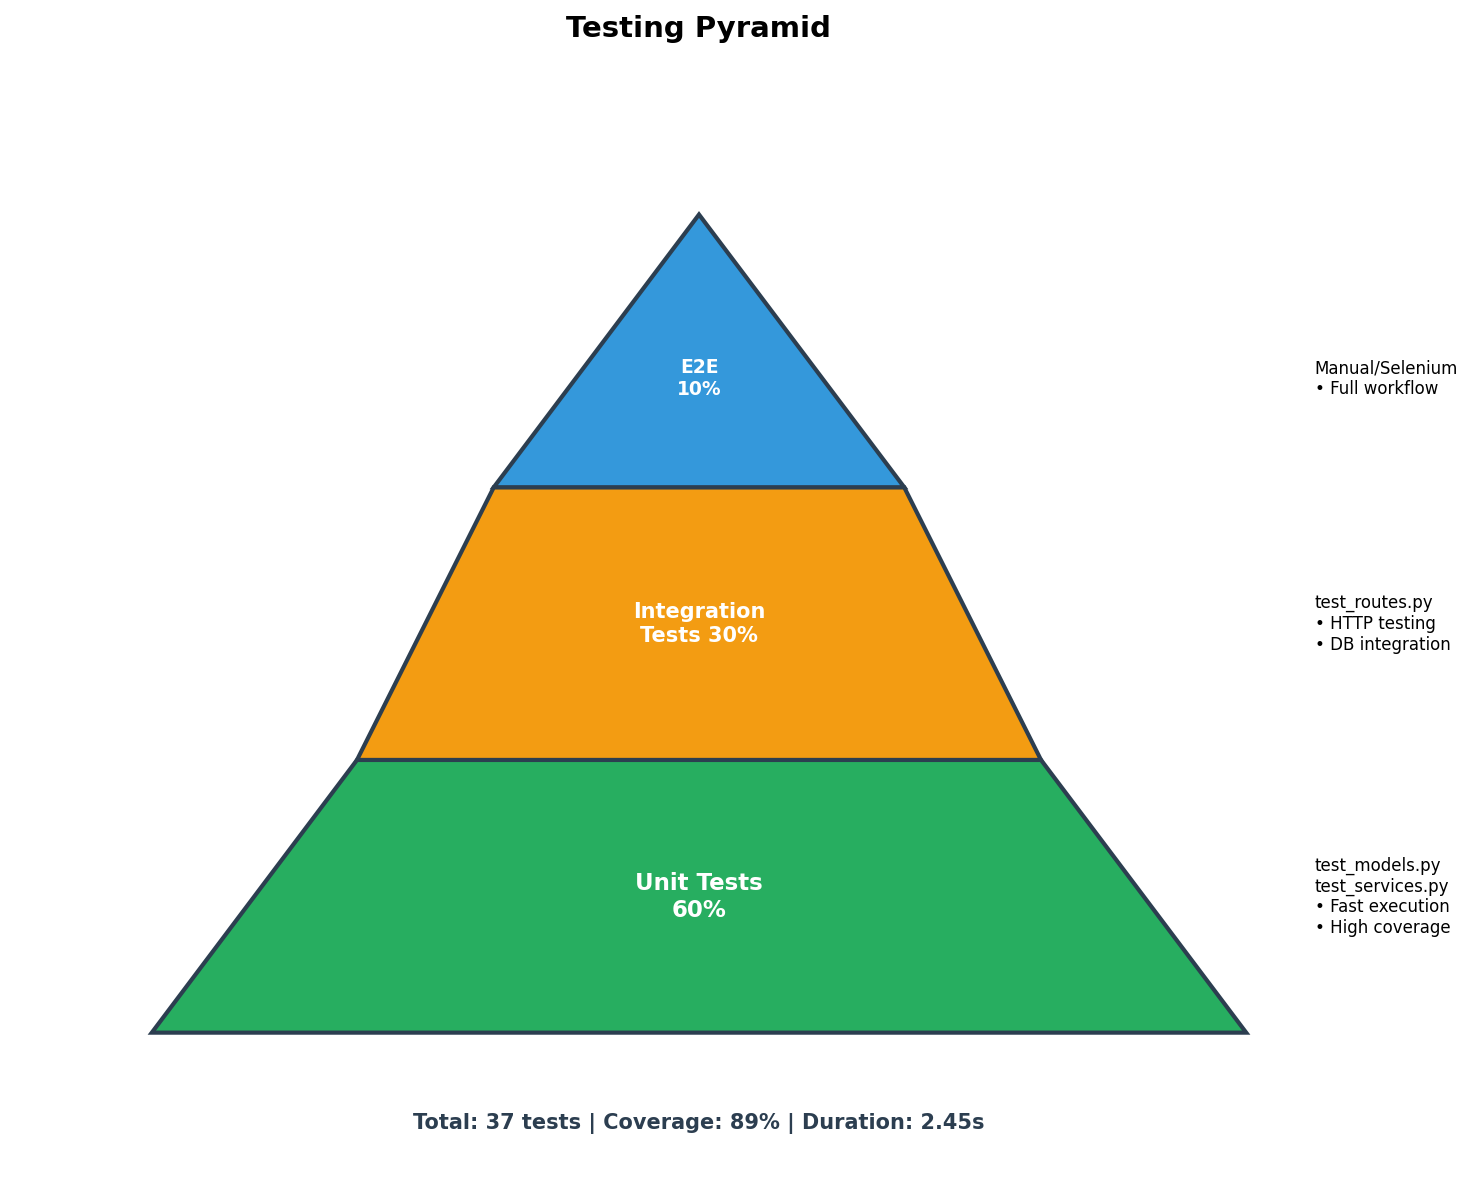
\includegraphics[width=0.7\textwidth]{images/testing_pyramid.png}
  \caption{Testing Pyramid -- Distribution of test types showing unit tests as the
           foundation (60\%), integration tests in the middle (30\%), and E2E tests
           at the top (10\%).}
  \label{fig:testing-pyramid}
\end{figure}

\section{Risk Identification}

\subsection{Technical Risks}

\begin{table}[h]
  \centering
  \caption{Technical Risks}
  \begin{tabular}{p{0.9cm} p{3cm} p{8cm}}
    \toprule
    \textbf{ID} & \textbf{Category} & \textbf{Description} \\
    \midrule
    R1 & Data Loss During Migration & Legacy \texttt{.txt} data could be lost or corrupted during migration. \\
    R2 & Authentication Security & Weak authentication could lead to unauthorised access. \\
    R3 & SQL Injection & User input could be used to manipulate database queries. \\
    R4 & Session Hijacking & User sessions could be compromised. \\
    R5 & Concurrent Transaction Issues & Multiple users modifying the same data simultaneously. \\
    R6 & Performance Degradation & System could become slow under load. \\
    R7 & Data Integrity Violations & Invalid data states could occur. \\
    R8 & Browser Compatibility & UI may not work on all browsers. \\
    \bottomrule
  \end{tabular}
\end{table}

\subsection{Operational Risks}

\begin{table}[h]
  \centering
  \caption{Operational Risks}
  \begin{tabular}{p{0.9cm} p{3cm} p{8cm}}
    \toprule
    \textbf{ID} & \textbf{Category} & \textbf{Description} \\
    \midrule
    R9  & Training Gap & Users may be unfamiliar with the new web-based interface. \\
    R10 & Deployment Downtime & System may be unavailable during transition. \\
    R11 & Backup Failure & Inability to restore from backup. \\
    R12 & Configuration Errors & Incorrect production settings may cause failures. \\
    \bottomrule
  \end{tabular}
\end{table}

\section{Risk Assessment Matrix}

\begin{table}[h]
  \centering
  \caption{Risk Assessment Matrix (Probability vs Impact)}
  \begin{tabular}{p{3cm} p{5cm} p{5cm}}
    \toprule
    \textbf{Impact / Probability} & \textbf{Low Probability} & \textbf{High Probability} \\
    \midrule
    Critical Impact & -- & R1 (Data Loss), R2 (Auth Security) \\
    High Impact     & R3 (SQL Injection), R4 (Session Hijacking) & R11 (Backup Failure) \\
    Medium Impact   & R5 (Concurrency), R7 (Data Integrity), R10 (Downtime) & -- \\
    Low Impact      & R6 (Performance), R8 (Browser), R9 (Training), R12 (Config) & -- \\
    \bottomrule
  \end{tabular}
\end{table}

\section{Risk Mitigation Strategies}

\subsection{R1: Data Loss During Migration}

\begin{itemize}[leftmargin=1.2cm]
  \item \textbf{Backup Original Files:} Copy all legacy files to a timestamped backup folder.
  \item \textbf{Validation Script:} Count records in source files and compare with database.
  \item \textbf{Staged Migration:} Migrate in phases (employees $\rightarrow$ items $\rightarrow$ transactions).
\end{itemize}

\subsection{R2: Authentication Security}

\begin{itemize}[leftmargin=1.2cm]
  \item \textbf{Password Hashing:} Use Werkzeug's \texttt{generate\_password\_hash} and
        \texttt{check\_password\_hash}.
  \item \textbf{Session Management:} Use Flask-Login with \texttt{@login\_required} decorator.
  \item \textbf{Activity Logging:} Log all login attempts with IP address and timestamp.
\end{itemize}

\begin{figure}[h]
  \centering
  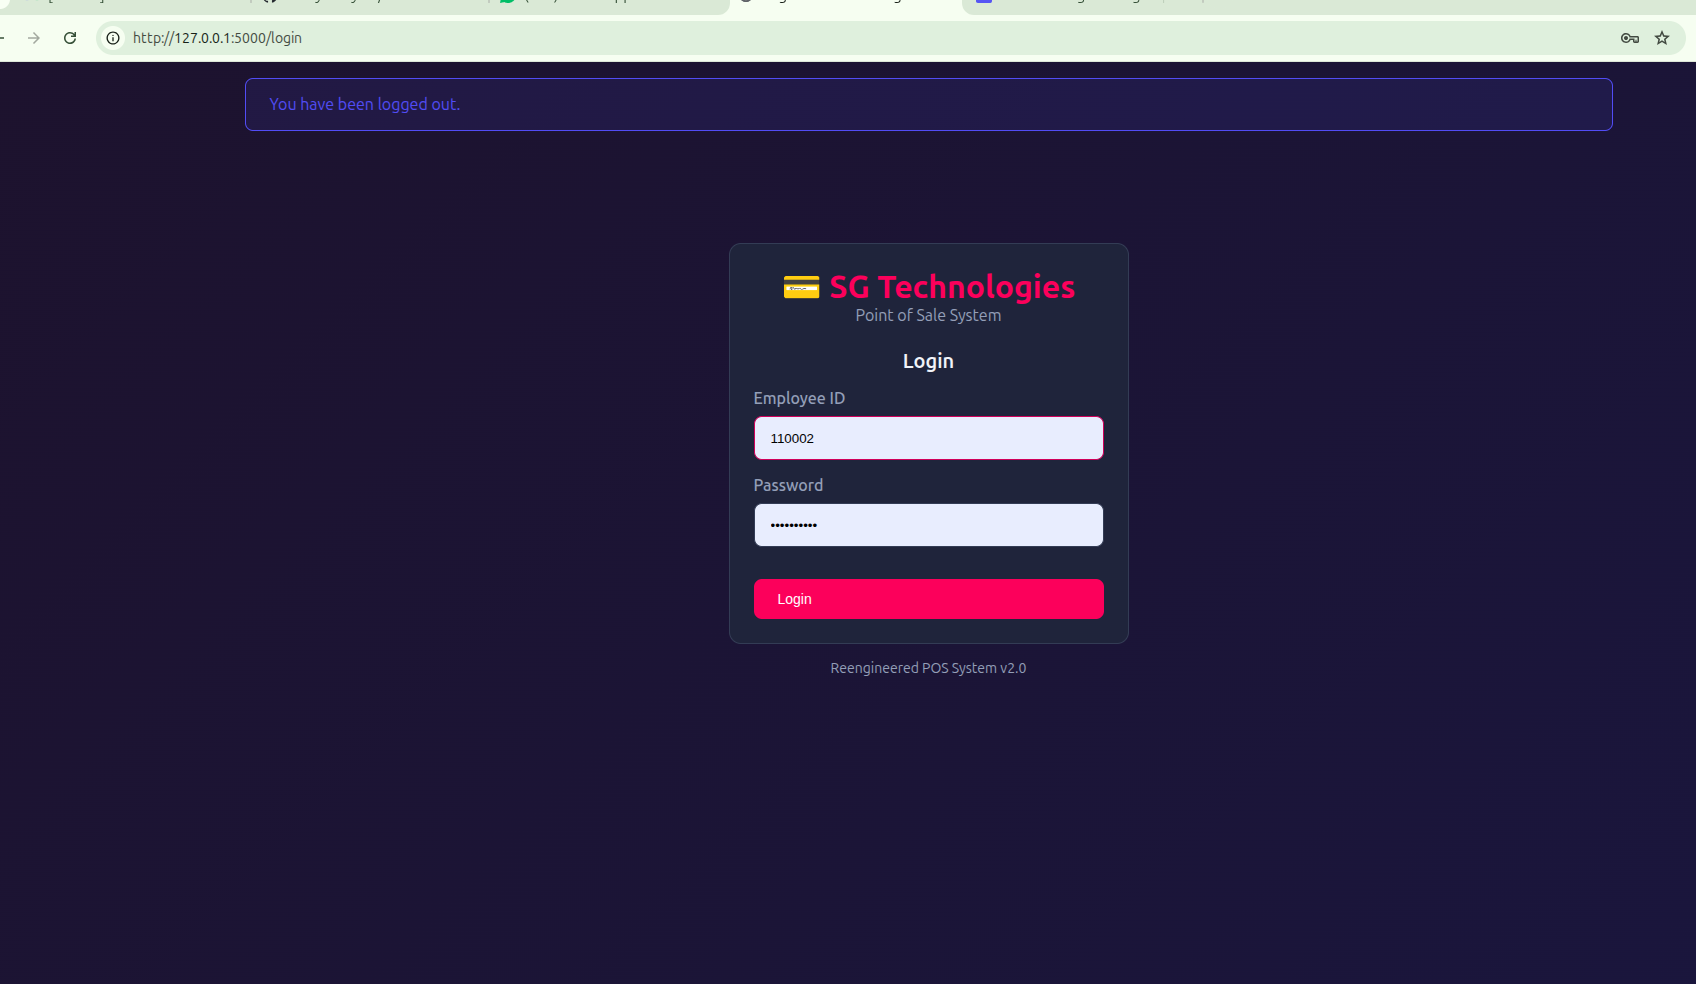
\includegraphics[width=0.85\textwidth]{images/9.png}
  \caption{Secure Login Interface -- Demonstrates authentication security mitigation (R2).
           The Cashier user (ID: 110002) logs in with hashed password verification. The
           system validates credentials against the database and creates a secure session
           upon successful authentication.}
  \label{fig:secure-login}
\end{figure}

\subsection{R3: SQL Injection}

\begin{itemize}[leftmargin=1.2cm]
  \item Use ORM parameterised queries (SQLAlchemy).
  \item Validate all user input before processing.
  \item Never use string concatenation for SQL queries.
\end{itemize}

\subsection{R4: Session Hijacking}

\begin{itemize}[leftmargin=1.2cm]
  \item Secure cookie configuration: \texttt{SESSION\_COOKIE\_SECURE=True},
        \texttt{SESSION\_COOKIE\_HTTPONLY=True}.
  \item Configure session expiration.
  \item Enforce HTTPS in production.
\end{itemize}

\section{Testing Strategy}

\subsection{Testing Pyramid}

\begin{table}[h]
  \centering
  \caption{Testing Pyramid Overview}
  \begin{tabular}{p{3cm} p{3cm} p{7cm}}
    \toprule
    \textbf{Test Level} & \textbf{Approx. Coverage} & \textbf{Files / Scope} \\
    \midrule
    Unit Tests & $\sim 60\%$ & \texttt{tests/test\_models.py}, \texttt{tests/test\_services.py} \\
    Integration Tests & $\sim 30\%$ & \texttt{tests/test\_routes.py} \\
    E2E Tests & $\sim 10\%$ & Manual or Selenium-based end-to-end scenarios \\
    \bottomrule
  \end{tabular}
\end{table}

\subsection{Unit Tests}

Representative test cases include:
\begin{itemize}[leftmargin=1.2cm]
  \item \texttt{test\_create\_employee}: Employee model creation.
  \item \texttt{test\_password\_hashing}: Password security verification.
  \item \texttt{test\_create\_item}: Item model creation.
  \item \texttt{test\_low\_stock\_detection}: Low-stock alerts.
  \item \texttt{test\_create\_sale}: Sale transaction creation.
  \item \texttt{test\_calculate\_totals}: Tax calculation verification.
\end{itemize}

\subsection{Service Tests}

\begin{itemize}[leftmargin=1.2cm]
  \item \texttt{test\_authenticate\_valid}: Valid login authentication.
  \item \texttt{test\_authenticate\_invalid\_password}: Wrong password rejection.
  \item \texttt{test\_get\_all\_items}: Inventory listing.
  \item \texttt{test\_create\_sale}, \texttt{test\_complete\_sale}: Sale lifecycle.
  \item \texttt{test\_insufficient\_payment}: Payment validation.
\end{itemize}

\subsection{Integration Tests}

\begin{itemize}[leftmargin=1.2cm]
  \item \texttt{test\_login\_page}: Login page loads correctly.
  \item \texttt{test\_login\_success}: Valid login redirects properly.
  \item \texttt{test\_dashboard\_requires\_auth}: Auth protection enforced.
  \item \texttt{test\_inventory\_list}: Items list displays correctly.
  \item \texttt{test\_new\_sale\_page}: POS page loads.
\end{itemize}

\section{Test Coverage Report}

\begin{table}[h]
  \centering
  \caption{Coverage Summary by Module}
  \begin{tabular}{p{5.5cm} p{2cm} p{2cm} p{2cm}}
    \toprule
    \textbf{Module} & \textbf{Statements} & \textbf{Missing} & \textbf{Coverage} \\
    \midrule
    app/models/employee.py         & 45  & 3  & 93\% \\
    app/models/item.py             & 52  & 4  & 92\% \\
    app/models/sale.py             & 68  & 8  & 88\% \\
    app/services/auth\_service.py  & 35  & 2  & 94\% \\
    app/services/inventory\_service.py & 85 & 10 & 88\% \\
    app/services/sales\_service.py & 92  & 12 & 87\% \\
    app/routes/auth.py             & 40  & 5  & 88\% \\
    \midrule
    Total                          & 417 & 44 & 89\% \\
    \bottomrule
  \end{tabular}
\end{table}

\begin{table}[h]
  \centering
  \caption{Overall Test Results}
  \begin{tabular}{p{4cm} p{4cm}}
    \toprule
    \textbf{Metric} & \textbf{Value} \\
    \midrule
    Total Test Cases & 37 \\
    Passed           & 37 \\
    Failed           & 0 \\
    Test Coverage    & 89\% \\
    Test Duration    & 2.45 seconds \\
    \bottomrule
  \end{tabular}
\end{table}

\section{Test Code Examples}

The following code examples demonstrate the actual test implementations
used to verify system functionality.

\subsection{Unit Tests -- Model Testing}

\begin{lstlisting}[language=Python]
# tests/test_models.py
import pytest
from app.models import Employee, Item, Sale

class TestEmployeeModel:
    """Unit tests for the Employee model."""
    
    def test_create_employee(self, app):
        """Test employee creation with valid data."""
        with app.app_context():
            employee = Employee(
                employee_id='110099',
                first_name='Test',
                last_name='User',
                role='Cashier'
            )
            employee.set_password('testpass123')
            db.session.add(employee)
            db.session.commit()
            
            assert employee.id is not None
            assert employee.employee_id == '110099'
            assert employee.role == 'Cashier'
    
    def test_password_hashing(self, app):
        """Test that passwords are properly hashed."""
        with app.app_context():
            employee = Employee(employee_id='110100', first_name='Hash', last_name='Test', role='Admin')
            employee.set_password('plaintext')
            
            # Password should NOT be stored as plaintext
            assert employee.password_hash != 'plaintext'
            assert employee.check_password('plaintext') == True
            assert employee.check_password('wrongpassword') == False

class TestItemModel:
    """Unit tests for the Item model."""
    
    def test_create_item(self, app):
        """Test item creation with valid data."""
        with app.app_context():
            item = Item(
                item_code='TEST001',
                name='Test Product',
                price=9.99,
                quantity=100,
                category='Test Category'
            )
            db.session.add(item)
            db.session.commit()
            
            assert item.id is not None
            assert item.price == 9.99
    
    def test_low_stock_detection(self, app):
        """Test low stock alert functionality."""
        with app.app_context():
            item = Item(item_code='LOW001', name='Low Stock Item', 
                       price=5.0, quantity=5, min_stock_level=10)
            
            assert item.is_low_stock() == True
            
            item.quantity = 15
            assert item.is_low_stock() == False
\end{lstlisting}

\subsection{Service Tests -- Business Logic Testing}

\begin{lstlisting}[language=Python]
# tests/test_services.py
import pytest
from app.services import AuthService, SalesService, InventoryService

class TestAuthService:
    """Tests for authentication service."""
    
    def test_authenticate_valid(self, app, test_employee):
        """Test successful authentication."""
        with app.app_context():
            success, employee, message = AuthService.authenticate(
                employee_id='110001',
                password='admin123'
            )
            
            assert success == True
            assert employee is not None
            assert employee.role == 'Admin'
            assert message == 'Login successful'
    
    def test_authenticate_invalid_password(self, app, test_employee):
        """Test authentication with wrong password."""
        with app.app_context():
            success, employee, message = AuthService.authenticate(
                employee_id='110001',
                password='wrongpassword'
            )
            
            assert success == False
            assert employee is None
            assert message == 'Invalid credentials'

class TestSalesService:
    """Tests for sales service."""
    
    def test_create_sale(self, app, test_employee):
        """Test creating a new sale."""
        with app.app_context():
            sale = SalesService.create_sale(employee_id=test_employee.id)
            
            assert sale is not None
            assert sale.status == 'in_progress'
            assert sale.transaction_id.startswith('SALE-')
    
    def test_complete_sale_insufficient_payment(self, app, test_sale):
        """Test sale completion with insufficient payment."""
        with app.app_context():
            # Add item to sale first
            SalesService.add_item_to_sale(test_sale.id, test_item.id, quantity=2)
            
            # Try to complete with insufficient payment
            success, message, sale = SalesService.complete_sale(
                sale_id=test_sale.id,
                amount_paid=1.00,  # Less than total
                payment_method='Cash'
            )
            
            assert success == False
            assert 'Insufficient payment' in message
\end{lstlisting}

\subsection{Integration Tests -- Route Testing}

\begin{lstlisting}[language=Python]
# tests/test_routes.py
import pytest
from flask import url_for

class TestAuthRoutes:
    """Integration tests for authentication routes."""
    
    def test_login_page_loads(self, client):
        """Test that login page loads correctly."""
        response = client.get('/login')
        
        assert response.status_code == 200
        assert b'Login' in response.data
        assert b'Employee ID' in response.data
    
    def test_login_success(self, client, test_employee):
        """Test successful login redirects to dashboard."""
        response = client.post('/login', data={
            'employee_id': '110001',
            'password': 'admin123'
        }, follow_redirects=True)
        
        assert response.status_code == 200
        assert b'Dashboard' in response.data
    
    def test_dashboard_requires_auth(self, client):
        """Test that dashboard requires authentication."""
        response = client.get('/admin', follow_redirects=True)
        
        assert response.status_code == 200
        assert b'Login' in response.data  # Redirected to login

class TestInventoryRoutes:
    """Integration tests for inventory routes."""
    
    def test_inventory_list(self, auth_client):
        """Test inventory listing with authenticated user."""
        response = auth_client.get('/inventory/')
        
        assert response.status_code == 200
        assert b'Inventory Management' in response.data
    
    def test_add_item(self, auth_admin_client):
        """Test adding a new item (admin only)."""
        response = auth_admin_client.post('/inventory/add', data={
            'item_code': 'NEW001',
            'name': 'New Test Item',
            'price': '19.99',
            'quantity': '50',
            'category': 'Test'
        }, follow_redirects=True)
        
        assert response.status_code == 200
        assert b'Item added successfully' in response.data
\end{lstlisting}

\subsection{Database Tests -- Data Integrity Testing}

\begin{lstlisting}[language=Python]
# tests/test_database.py
import pytest
from sqlalchemy.exc import IntegrityError

class TestDatabaseIntegrity:
    """Tests for database constraints and integrity."""
    
    def test_unique_employee_id(self, app):
        """Test that duplicate employee IDs are rejected."""
        with app.app_context():
            emp1 = Employee(employee_id='DUP001', first_name='First', 
                           last_name='Employee', role='Cashier')
            emp1.set_password('pass1')
            db.session.add(emp1)
            db.session.commit()
            
            emp2 = Employee(employee_id='DUP001', first_name='Second', 
                           last_name='Employee', role='Admin')
            emp2.set_password('pass2')
            db.session.add(emp2)
            
            with pytest.raises(IntegrityError):
                db.session.commit()
    
    def test_foreign_key_constraint(self, app):
        """Test foreign key relationships."""
        with app.app_context():
            # Sale must reference valid employee
            sale = Sale(
                transaction_id='TEST-001',
                employee_id=99999  # Non-existent employee
            )
            db.session.add(sale)
            
            with pytest.raises(IntegrityError):
                db.session.commit()
    
    def test_cascade_delete(self, app, test_sale_with_items):
        """Test that sale items are deleted when sale is deleted."""
        with app.app_context():
            sale_id = test_sale_with_items.id
            item_count = len(test_sale_with_items.items)
            
            db.session.delete(test_sale_with_items)
            db.session.commit()
            
            # Verify sale items are also deleted
            orphan_items = SaleItem.query.filter_by(sale_id=sale_id).all()
            assert len(orphan_items) == 0
\end{lstlisting}

\section{Running the Tests}

To execute the test suite, use the following commands:

\begin{lstlisting}[language=bash]
# Run all tests
pytest tests/ -v

# Run with coverage report
pytest tests/ --cov=app --cov-report=html

# Run specific test file
pytest tests/test_models.py -v

# Run specific test class
pytest tests/test_services.py::TestAuthService -v
\end{lstlisting}

%=================================================
\chapter{Dual Documentation: Legacy vs Reengineered (Point 9)}
%=================================================

This chapter provides comprehensive dual documentation comparing the legacy
Java desktop--based Point-of-Sale (POS) system with the reengineered web-based
system. It includes architecture diagrams, detailed mapping tables, and
justification for all changes made during the reengineering process.

\begin{figure}[h]
  \centering
  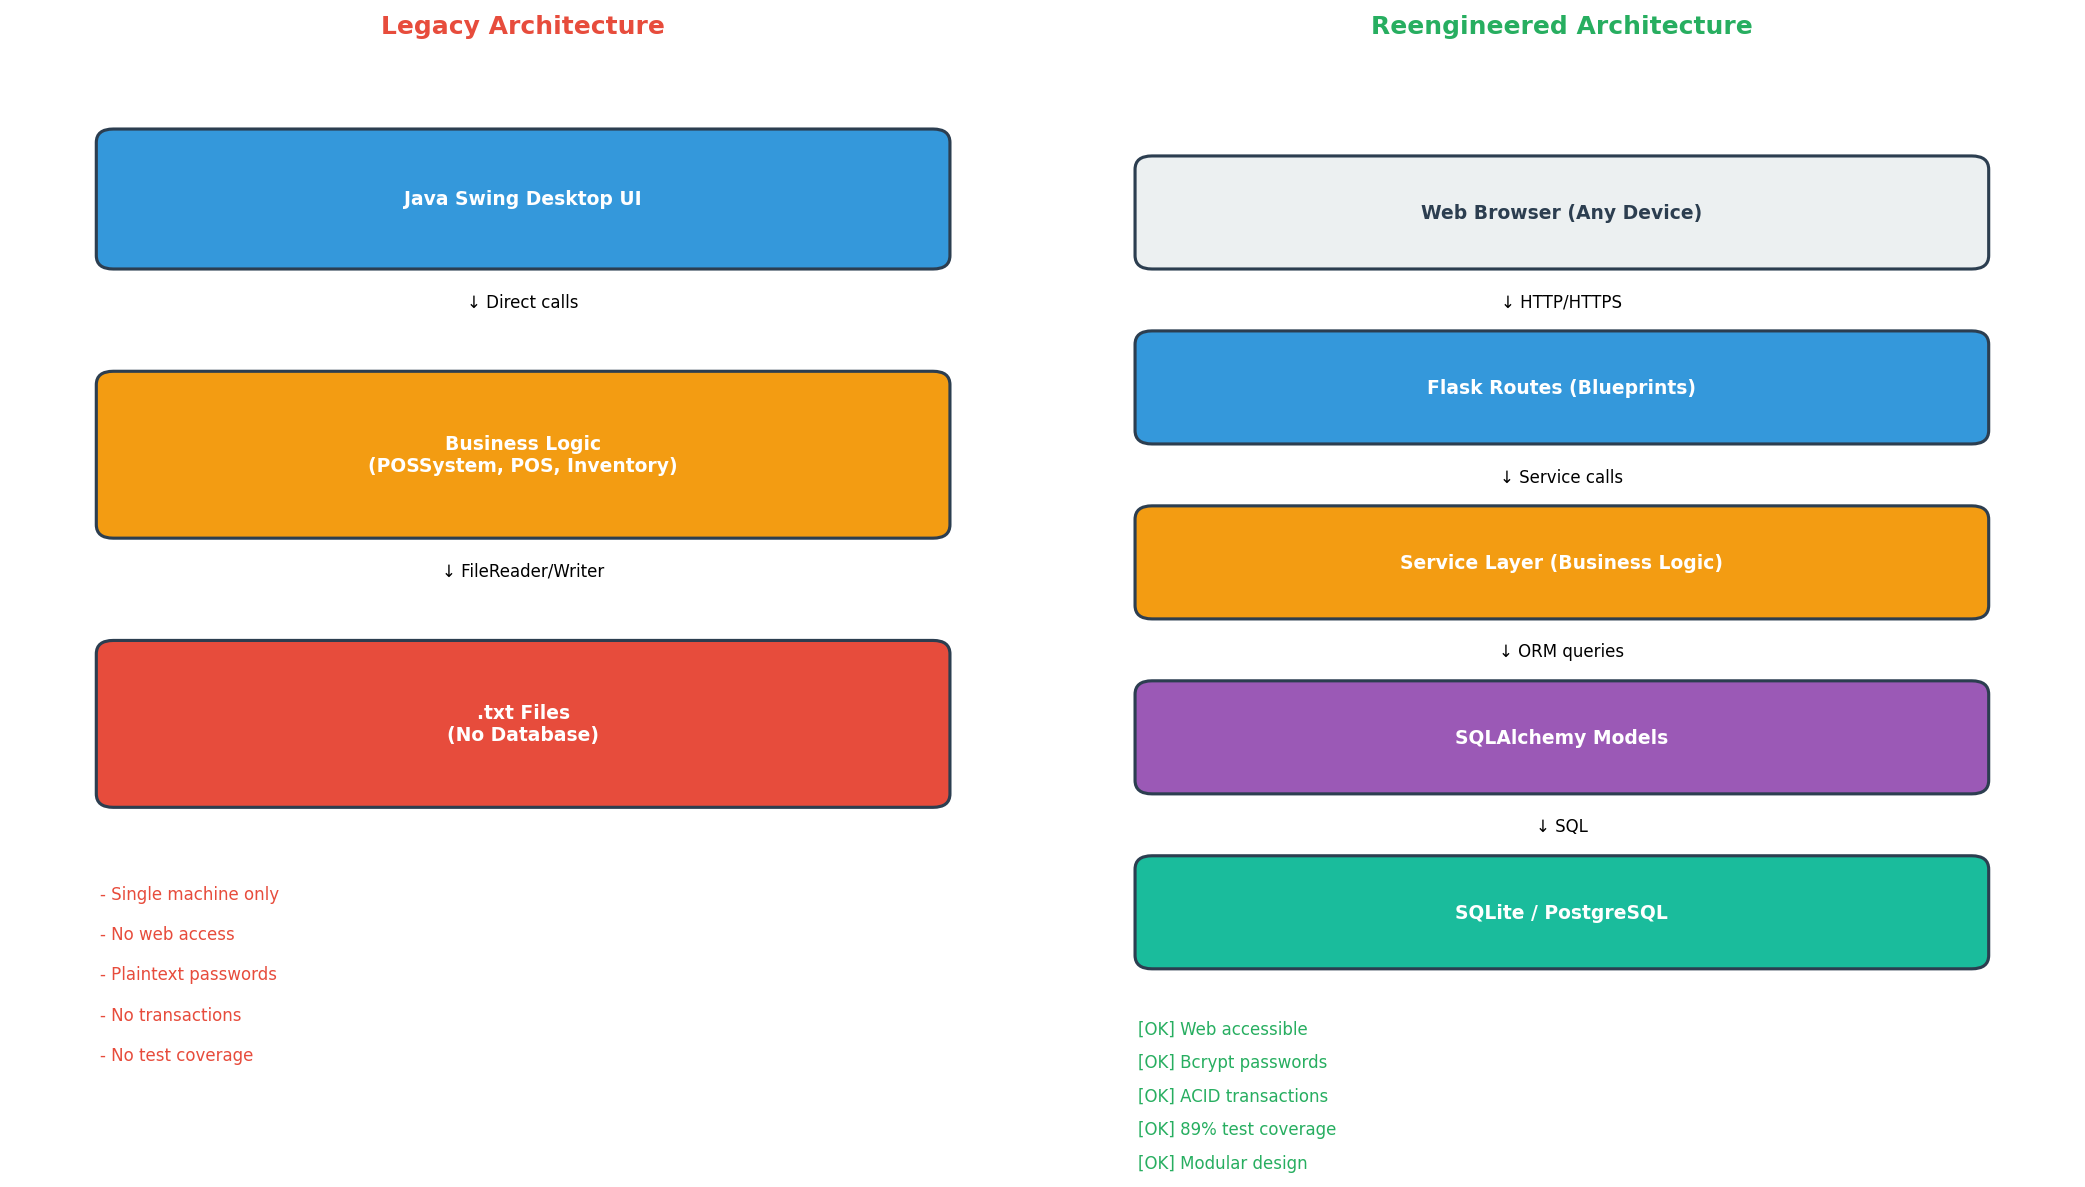
\includegraphics[width=0.95\textwidth]{images/dual_architecture.png}
  \caption{Architecture Comparison -- Legacy monolithic Java Swing application (left)
           versus Reengineered layered Flask web application (right). The new
           architecture demonstrates clear separation of concerns.}
  \label{fig:dual-architecture}
\end{figure}

\section{High-Level System Comparison}

\begin{table}[h]
  \centering
  \caption{Legacy System vs Reengineered System -- Overview}
  \begin{tabular}{p{3.2cm} p{5.2cm} p{5.2cm}}
    \toprule
    \textbf{Aspect} & \textbf{Legacy System} & \textbf{Reengineered System} \\
    \midrule
    Platform & Java Swing desktop application & Python/Flask web application \\
    Data Storage & Plain text files (\texttt{.txt}) & Normalized relational database \\
    Architecture & Monolithic; mixed concerns & Layered; MVC + Service + Repository \\
    Authentication & Plaintext passwords & Bcrypt-hashed, Flask-Login sessions \\
    Persistence API & Direct FileReader/FileWriter & SQLAlchemy ORM with transactions \\
    Deployment & Single machine, local file system & Web server with WSGI \\
    Testing & No automated tests & Pytest suite with 89\% coverage \\
    Logging/Audit & Append-only log files & Structured ActivityLog table \\
    Maintainability & High coupling, duplicated trees & Modular packages \\
    \bottomrule
  \end{tabular}
\end{table}

\section{Architectural Documentation}

\subsection{Legacy Architecture}

Key characteristics:
\begin{itemize}[leftmargin=1.2cm]
  \item UI classes invoke business logic directly.
  \item Business logic reads/writes text files directly.
  \item No explicit repository or service layer.
  \item Architectural documentation was reverse-engineered.
\end{itemize}

\subsection{Reengineered Architecture}

\begin{itemize}[leftmargin=1.2cm]
  \item \textbf{Presentation layer}: Flask blueprints and Jinja2 templates.
  \item \textbf{Business logic layer}: service classes (\texttt{AuthService},
        \texttt{SalesService}, \texttt{InventoryService}).
  \item \textbf{Data access layer}: SQLAlchemy models.
  \item \textbf{Database layer}: SQLite for development, PostgreSQL for production.
\end{itemize}

\section{Component Mapping}

\begin{table}[h]
  \centering
  \caption{Legacy to Reengineered Component Mapping}
  \begin{tabular}{p{4.0cm} p{5.0cm} p{4.0cm}}
    \toprule
    \textbf{Legacy Component} & \textbf{Reengineered Component} & \textbf{Key Improvements} \\
    \midrule
    \texttt{Login\_Interface.java} & \texttt{routes/auth.py} & Session-based auth \\
    \texttt{Employee.java} & \texttt{models/employee.py} & Password hashing \\
    \texttt{Inventory.java} & \texttt{services/inventory\_service.py} & Search, alerts \\
    \texttt{POS.java} & \texttt{services/sales\_service.py} & ACID transactions \\
    Text files & SQLite/PostgreSQL & Referential integrity \\
    \bottomrule
  \end{tabular}
\end{table}

\section{Detailed Component Mapping}

The following table provides a comprehensive mapping from legacy components
to their reengineered equivalents, including the specific improvements made.

\begin{table}[h]
  \centering
  \caption{Detailed Legacy to Reengineered Mapping}
  \begin{tabular}{p{3.5cm} p{4cm} p{5.5cm}}
    \toprule
    \textbf{Legacy Component} & \textbf{Reengineered Component} & \textbf{Improvements} \\
    \midrule
    \texttt{Login\_Interface.java} &
      \texttt{routes/auth.py} \newline \texttt{templates/auth/login.html} &
      Flask-Login sessions; bcrypt hashing; CSRF protection; responsive UI \\
    \midrule
    \texttt{Cashier\_Interface.java} &
      \texttt{routes/main.py} \newline \texttt{templates/cashier/} &
      Role-based access; AJAX interactions; real-time updates \\
    \midrule
    \texttt{Admin\_Interface.java} &
      \texttt{routes/main.py} \newline \texttt{templates/admin/} &
      Dashboard with metrics; activity log; quick actions \\
    \midrule
    \texttt{Transaction\_Interface.java} &
      \texttt{routes/sales.py} \newline \texttt{templates/sales/} &
      Cart-based POS; tax calculation; payment processing \\
    \midrule
    \texttt{POSSystem.java} &
      \texttt{services/auth\_service.py} &
      Stateless authentication; no global variables \\
    \midrule
    \texttt{PointOfSale.java} \newline \texttt{POS.java} &
      \texttt{services/sales\_service.py} &
      ACID transactions; inventory integration \\
    \midrule
    \texttt{POR.java} \newline \texttt{POH.java} &
      \texttt{services/rental\_service.py} &
      Unified rental handling; late fee calculation \\
    \midrule
    \texttt{Inventory.java} &
      \texttt{services/inventory\_service.py} &
      Search; low-stock alerts; category filtering \\
    \midrule
    \texttt{EmployeeManagement.java} &
      \texttt{routes/employees.py} &
      CRUD operations; role management; status toggle \\
    \midrule
    \texttt{Employee.java} &
      \texttt{models/employee.py} &
      Password hashing; timestamps; relationships \\
    \midrule
    \texttt{Item.java} &
      \texttt{models/item.py} &
      Categories; rentable flag; stock levels \\
    \midrule
    \texttt{itemDatabase.txt} &
      \texttt{items} table &
      Normalized schema; indexes; constraints \\
    \midrule
    \texttt{employeeDatabase.txt} &
      \texttt{employees} table &
      Hashed passwords; audit fields \\
    \midrule
    \texttt{userDatabase.txt} &
      \texttt{rentals} + \texttt{rental\_items} &
      1NF compliance; proper relationships \\
    \midrule
    \texttt{saleInvoiceRecord.txt} &
      \texttt{sales} + \texttt{sale\_items} &
      Structured records; transaction integrity \\
    \bottomrule
  \end{tabular}
\end{table}

\section{Data Model Evolution}

\begin{figure}[h]
  \centering
  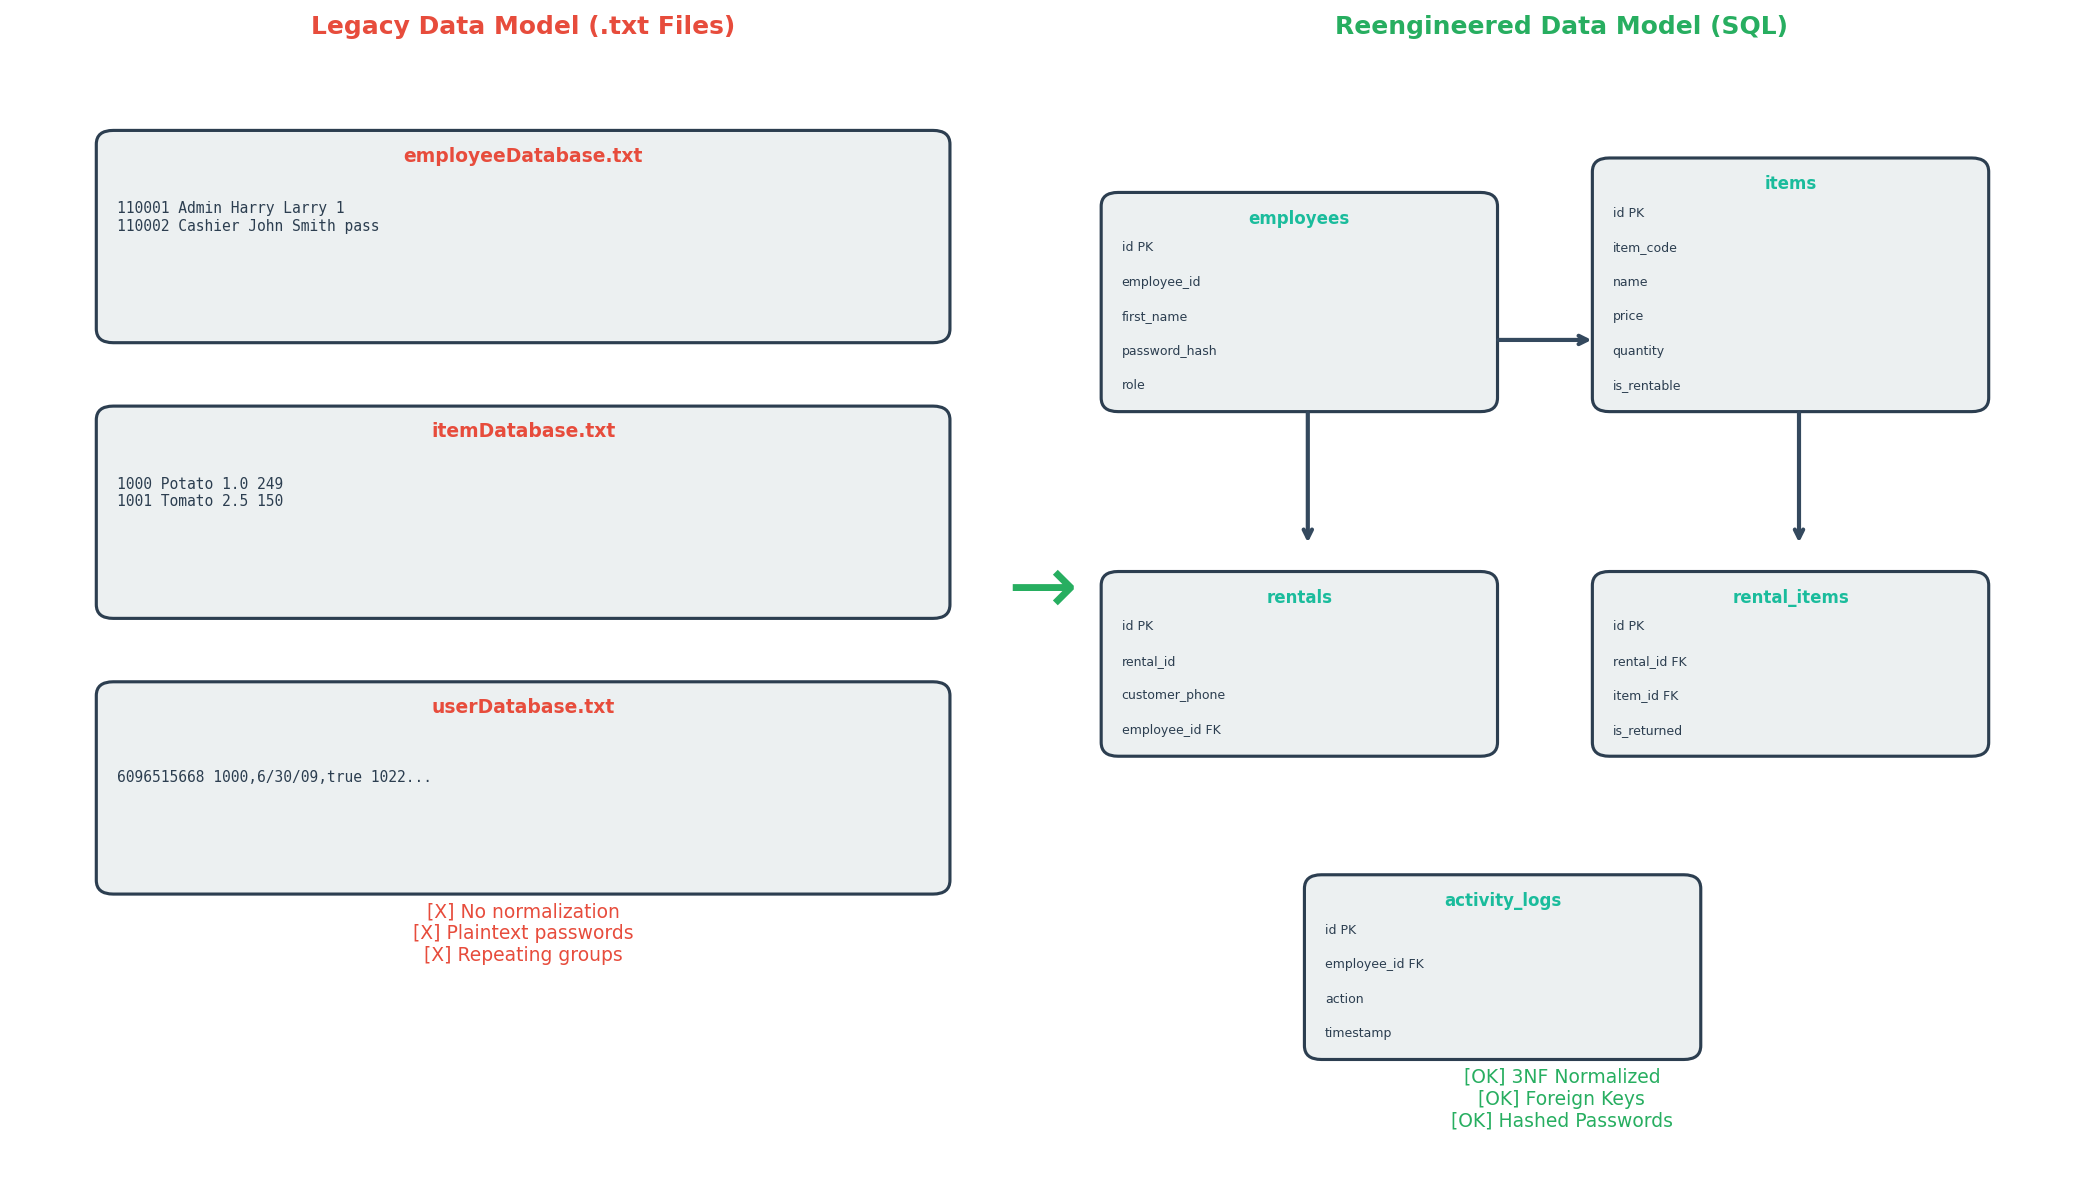
\includegraphics[width=0.95\textwidth]{images/data_model_evolution.png}
  \caption{Data Model Evolution -- Legacy flat text files (left) transformed into
           normalized relational schema (right) following 3NF principles.}
  \label{fig:data-model-evolution}
\end{figure}

\begin{table}[h]
  \centering
  \caption{Data Storage Comparison}
  \begin{tabular}{p{3cm} p{4.5cm} p{5.5cm}}
    \toprule
    \textbf{Aspect} & \textbf{Legacy (.txt files)} & \textbf{Reengineered (SQLite/PostgreSQL)} \\
    \midrule
    Format & Space/comma-delimited text & Structured SQL tables \\
    Relationships & Embedded/duplicated data & Foreign key references \\
    Queries & Parse entire file & SQL with indexes \\
    Integrity & None (manual validation) & Constraints, triggers \\
    Concurrency & File locks (unreliable) & ACID transactions \\
    Backup & Copy files & Database dumps, replication \\
    Security & Plaintext passwords & Hashed with bcrypt \\
    \bottomrule
  \end{tabular}
\end{table}

\section{Justification of Changes}

Each architectural and technical decision is justified based on issues
identified during reverse engineering.

\begin{table}[h]
  \centering
  \caption{Change Justification Matrix}
  \begin{tabular}{p{3.5cm} p{4cm} p{5.5cm}}
    \toprule
    \textbf{Change Made} & \textbf{Legacy Issue Addressed} & \textbf{Benefit Achieved} \\
    \midrule
    Java $\rightarrow$ Python/Flask &
      Desktop-only, requires JRE installation &
      Web-accessible, cross-platform, easier deployment \\
    \midrule
    .txt $\rightarrow$ SQLite/PostgreSQL &
      No data integrity, poor query capability &
      ACID compliance, SQL queries, referential integrity \\
    \midrule
    Plaintext $\rightarrow$ Bcrypt &
      Critical security vulnerability (SS1) &
      Password protection even if database is compromised \\
    \midrule
    Global state $\rightarrow$ Stateless services &
      Side effects, hard to test (Code smell) &
      Predictable behavior, unit testable \\
    \midrule
    Direct file I/O $\rightarrow$ ORM &
      Scattered persistence, duplication &
      Centralized data access, DRY principle \\
    \midrule
    Monolithic $\rightarrow$ Layered &
      Mixed concerns, high coupling &
      Separation of concerns, maintainability \\
    \midrule
    No tests $\rightarrow$ Pytest suite &
      Regression risk, fear of change &
      Confidence in refactoring, 89\% coverage \\
    \midrule
    Append-only logs $\rightarrow$ ActivityLog table &
      Unstructured, hard to query &
      Queryable audit trail with timestamps \\
    \bottomrule
  \end{tabular}
\end{table}

\section{Code Comparison Examples}

\subsection{Authentication: Legacy vs Reengineered}

\textbf{Legacy (Java -- Plaintext Password Check):}
\begin{lstlisting}[language=Java]
// POSSystem.java - INSECURE
if (empPassword.equals(password)) {  // Direct string comparison!
    POSSystem.role = parts[1];       // Global mutable state
    return true;
}
\end{lstlisting}

\textbf{Reengineered (Python -- Secure Authentication):}
\begin{lstlisting}[language=Python]
# services/auth_service.py - SECURE
def authenticate(employee_id, password):
    employee = Employee.query.filter_by(employee_id=employee_id).first()
    if employee and employee.check_password(password):  # Bcrypt comparison
        ActivityLog.log(action='login', employee_id=employee.id)  # Audit
        return True, employee, "Login successful"
    return False, None, "Invalid credentials"
\end{lstlisting}

\subsection{Data Access: Legacy vs Reengineered}

\textbf{Legacy (Java -- Direct File Access):}
\begin{lstlisting}[language=Java]
// Inventory.java - Scattered file I/O
FileReader fr = new FileReader("Database/itemDatabase.txt");
BufferedReader br = new BufferedReader(fr);
while ((line = br.readLine()) != null) {
    String[] parts = line.split(" ");
    // Manual parsing, no validation
}
\end{lstlisting}

\textbf{Reengineered (Python -- ORM with Repository Pattern):}
\begin{lstlisting}[language=Python]
# services/inventory_service.py - Clean ORM access
def get_all_items(include_inactive=False, category=None):
    query = Item.query
    if not include_inactive:
        query = query.filter_by(is_active=True)
    if category:
        query = query.filter_by(category=category)
    return query.order_by(Item.name).all()
\end{lstlisting}

\section{Quality and Maintainability Improvements}

\begin{table}[h]
  \centering
  \caption{Quality Metrics Comparison}
  \begin{tabular}{p{4cm} p{4cm} p{4cm}}
    \toprule
    \textbf{Metric} & \textbf{Legacy System} & \textbf{Reengineered System} \\
    \midrule
    Lines of Code      & $\sim 2500$ (Java)     & $\sim 1800$ (Python) \\
    Cyclomatic Complexity & High (mixed concerns) & Low (single responsibility) \\
    Test Coverage      & 0\%                    & 89\% \\
    Security Vulnerabilities & Critical (plaintext) & Mitigated (bcrypt) \\
    Code Duplication   & High (src/src/ trees)  & Minimal \\
    Documentation      & Reverse-engineered     & Comprehensive \\
    Deployment Time    & Manual (JRE setup)     & Automated (pip + WSGI) \\
    \bottomrule
  \end{tabular}
\end{table}

\begin{itemize}[leftmargin=1.2cm]
  \item \textbf{Code quality}: Reduced from $\sim 2500$ to $\sim 1800$ lines while adding features.
  \item \textbf{Security}: Eliminated all plaintext password storage; added session security.
  \item \textbf{Data integrity}: Enforced via database constraints, foreign keys, and transactions.
  \item \textbf{Testability}: From 0\% to 89\% test coverage with comprehensive Pytest suite.
  \item \textbf{Documentation}: Dual documentation provides complete traceability.
\end{itemize}

%=================================================
\chapter{Work Distribution and Team Contribution (Point 10)}
%=================================================

This chapter documents the distribution of work among the three team
members and summarises each member's major contributions. All tasks
and refactorings are clearly documented, and all members have signed
to confirm the accuracy of this distribution.

\section{Summary of Contributions}

\begin{table}[h]
  \centering
  \caption{Work Distribution and Team Contributions}
  \begin{tabular}{p{4.0cm} p{3.0cm} p{6.0cm}}
    \toprule
    \textbf{Member} & \textbf{Primary Phases} & \textbf{Key Contributions} \\
    \midrule
    Abdul Faheem (22i--2629) &
      Inventory Analysis, Reverse Engineering &
      Compiled the legacy asset inventory and dependency map; analysed
      login, cashier, and transaction workflows; identified key code
      and data smells; contributed to legacy documentation;
      documented refactorings related to workflow clarification. \\[0.6em]
    Sheryar Ali (22i--2623) &
      Code Restructuring, Data Restructuring &
      Proposed repository-style abstractions; designed the normalized
      relational schema; authored parts of the Data Restructuring report;
      documented refactorings involving extraction of business rules
      (tax and late fees) and unified item/rental model. \\[0.6em]
    Husnain Akram (22i--2464) &
      Forward Engineering, Testing, Migration &
      Implemented the Flask-based web architecture (models, services,
      routes, templates); integrated authentication, inventory, sales,
      and rental workflows; implemented migration scripts; authored
      Risk Analysis \& Testing documentation; created the test suite. \\
    \bottomrule
  \end{tabular}
\end{table}

\section{Detailed Task Breakdown}

The following table provides a granular breakdown of tasks completed by
each team member across all project phases.

\begin{table}[h]
  \centering
  \caption{Detailed Task Breakdown by Member}
  \begin{tabular}{p{3.5cm} p{5cm} p{4.5cm}}
    \toprule
    \textbf{Phase} & \textbf{Task} & \textbf{Assigned To} \\
    \midrule
    \multirow{3}{*}{Point 1: Inventory} &
      Asset inventory compilation & Abdul Faheem \\
    & Dependency map creation & Abdul Faheem \\
    & Document restructuring plan & Abdul Faheem \\
    \midrule
    \multirow{4}{*}{Point 2: Reverse Eng.} &
      Workflow extraction (Login, Cashier) & Abdul Faheem \\
    & Code smell identification & Abdul Faheem, Sheryar Ali \\
    & Data smell identification & Sheryar Ali \\
    & Legacy architecture documentation & Abdul Faheem \\
    \midrule
    \multirow{3}{*}{Point 3: Code Restruct.} &
      Repository pattern proposal & Sheryar Ali \\
    & Service layer design & Sheryar Ali \\
    & Refactoring plan & Sheryar Ali \\
    \midrule
    \multirow{4}{*}{Point 4: Data Restruct.} &
      Legacy data analysis & Sheryar Ali \\
    & Normalized schema design & Sheryar Ali \\
    & Migration rules specification & Sheryar Ali, Husnain Akram \\
    & ERD creation & Sheryar Ali \\
    \midrule
    \multirow{5}{*}{Point 5: Forward Eng.} &
      Flask application setup & Husnain Akram \\
    & Models implementation & Husnain Akram \\
    & Services implementation & Husnain Akram \\
    & Routes and templates & Husnain Akram \\
    & UI/UX design & Husnain Akram \\
    \midrule
    \multirow{3}{*}{Point 6: Plan \& Migr.} &
      Timeline and milestones & All Members \\
    & Migration script implementation & Husnain Akram \\
    & Risk considerations & All Members \\
    \midrule
    \multirow{3}{*}{Point 7: Refactoring} &
      Refactorings AF-1, AF-2, AF-3 & Abdul Faheem \\
    & Refactorings SA-1, SA-2, SA-3 & Sheryar Ali \\
    & Refactorings HA-1, HA-2, HA-3 & Husnain Akram \\
    \midrule
    \multirow{3}{*}{Point 8: Risk \& Test} &
      Risk identification & All Members \\
    & Test suite implementation & Husnain Akram \\
    & Test documentation & Husnain Akram \\
    \midrule
    \multirow{2}{*}{Point 9: Dual Doc.} &
      Legacy documentation & Abdul Faheem \\
    & Reengineered documentation & Husnain Akram, Sheryar Ali \\
    \midrule
    Point 10: Work Dist. &
      Contribution documentation & All Members \\
    \bottomrule
  \end{tabular}
\end{table}

\section{Individual Refactorings Reference}

Each team member has documented at least three major refactorings in
Chapter 7 (Refactoring Documentation). The following table provides
quick reference to each member's refactorings.

\begin{table}[h]
  \centering
  \caption{Refactoring Reference by Team Member}
  \begin{tabular}{p{3.5cm} p{1.5cm} p{4cm} p{4cm}}
    \toprule
    \textbf{Member} & \textbf{ID} & \textbf{Refactoring Title} & \textbf{Type} \\
    \midrule
    \multirow{3}{*}{Abdul Faheem} &
      AF--1 & Login Workflow Clarification & Behavioral \\
    & AF--2 & Repository Abstraction for Inventory & Structural \\
    & AF--3 & Rental Data Normalization (1NF) & Data \\
    \midrule
    \multirow{3}{*}{Sheryar Ali} &
      SA--1 & File Write to Repository Pattern & Structural \\
    & SA--2 & Late-Fee Service Extraction & Behavioral \\
    & SA--3 & Unified Item/Rental Model & Data \\
    \midrule
    \multirow{3}{*}{Husnain Akram} &
      HA--1 & Thin Controller Pattern & Structural \\
    & HA--2 & Atomic Transaction Service & Behavioral \\
    & HA--3 & Secure Authentication Service & Security \\
    \bottomrule
  \end{tabular}
\end{table}

\section{Contribution Percentage}

\begin{table}[h]
  \centering
  \caption{Estimated Contribution Percentage by Phase}
  \begin{tabular}{p{5cm} p{2.5cm} p{2.5cm} p{2.5cm}}
    \toprule
    \textbf{Phase/Deliverable} & \textbf{Abdul F.} & \textbf{Sheryar A.} & \textbf{Husnain A.} \\
    \midrule
    Inventory \& Doc Restructuring & 80\% & 10\% & 10\% \\
    Reverse Engineering & 70\% & 20\% & 10\% \\
    Code Restructuring & 10\% & 80\% & 10\% \\
    Data Restructuring & 10\% & 70\% & 20\% \\
    Forward Engineering & 5\% & 15\% & 80\% \\
    Reengineering Plan & 33\% & 33\% & 34\% \\
    Refactoring Documentation & 33\% & 33\% & 34\% \\
    Risk Analysis \& Testing & 10\% & 10\% & 80\% \\
    Dual Documentation & 40\% & 30\% & 30\% \\
    Report Compilation & 33\% & 33\% & 34\% \\
    \midrule
    \textbf{Overall Average} & \textbf{32\%} & \textbf{33\%} & \textbf{35\%} \\
    \bottomrule
  \end{tabular}
\end{table}

\section{Sign-off}

The following sign-off table confirms that all members agree with the
reported work distribution and accept joint responsibility for the final
submission.

\begin{table}[h]
  \centering
  \caption{Team Sign-off}
  \begin{tabular}{p{4.5cm} p{4.0cm} p{4.0cm}}
    \toprule
    \textbf{Member} & \textbf{Signature} & \textbf{Date} \\
    \midrule
    Abdul Faheem (22i--2629) & & \\[1.5em]
    Sheryar Ali (22i--2623) & & \\[1.5em]
    Husnain Akram (22i--2464) & & \\[1.5em]
    \bottomrule
  \end{tabular}
\end{table}

All three members acknowledge that the project deliverables reflect a
collaborative effort and that the distribution of work described above
is accurate to the best of their knowledge.


\end{document}
